\documentclass[a4paper,12pt]{scrreprt}
\usepackage[left= 2.5cm,right = 2cm, bottom = 4 cm]{geometry}
\usepackage[english]{babel}
\usepackage[table,xcdraw]{xcolor}
\usepackage[utf8x]{inputenc}
\usepackage{ucs}
\usepackage{wrapfig}
\usepackage{pdfpages}
\usepackage{graphicx}
\usepackage{acronym}
\usepackage{eurosym}
\usepackage[linktocpage=true]{hyperref}
\usepackage[autostyle=true,german=quotes]{csquotes}
\usepackage{caption}
\usepackage{subcaption}
\usepackage{float}
\usepackage{scrhack}
\usepackage{tikz}
\usepackage{multirow}
\usepackage{wrapfig}  
\usepackage{listings}
\usepackage{color}
\usepackage{tabularx}
\usepackage[table,xcdraw]{xcolor}
\usepackage{vhistory}
\usepackage{amsmath}
\usepackage{multicol}
\usepackage{enumitem}
\usepackage{lscape}
\usepackage{graphicx}
\usepackage{pdfpages} 

\usepackage[T1]{fontenc}          %versch. Schriftarten
\newcommand{\changefont}[3]{%
\fontfamily{#1}%
\fontseries{#2}%
\fontshape{#3}%
\selectfont}

% XML


\usepackage{color}
\definecolor{gray}{rgb}{0.4,0.4,0.4}
\definecolor{darkblue}{rgb}{0.0,0.0,0.6}
\definecolor{cyan}{rgb}{0.0,0.6,0.6}
\definecolor{weiss}{RGB}{255,255,255}
\definecolor{logoBlau}{RGB}{29,113,184}
\definecolor{logoGrau}{RGB}{87,87,86}

\makeatletter
\renewcommand{\overset}[2]{\ensuremath{\mathop{\kern\z@\mbox{#2}}\limits^{\mbox{\scriptsize #1}}}}
\renewcommand{\underset}[2]{\ensuremath{\mathop{\kern\z@\mbox{#2}}\limits_{\mbox{\scriptsize #1}}}}
\makeatother

%\mbox{}Without \verb|amsmath|: \overset{x}{a}~\quad~\underset{x}{a}

%\newcommand{\logo}{\textit{\textcolor{logoBlau}{grab}\textcolor{logoGrau}{tastic}\textsuperscript{\textcolor{logoGrau}{2015}}} }
\newcommand{\logoTitle}{%
\fontfamily{phv}\selectfont%
\textit{\textcolor{logoBlau}{grab}\textcolor{logoGrau}{%
tastic\overset{2015}{\textcolor{weiss}{=}}}%
}%
\normalfont}

\newcommand{\logo}{%
\fontfamily{phv}\selectfont%
\textit{\textcolor{%
logoBlau}{grab}\textcolor{logoGrau}{tastic }}%
\normalfont}

\lstdefinelanguage{XML}
{
  morestring=[b]",
  morestring=[s]{>}{<},
  morecomment=[s]{<?}{?>},
  stringstyle=\color{black},
  identifierstyle=\color{darkblue},
  keywordstyle=\color{cyan},
  morekeywords={xmlns,version,type}% list your attributes here
}

%\usepackage{subfigure} 
\usepackage[T1]{fontenc}
\captionsetup{format=hang, justification=raggedright}
\usepackage[sort]{natbib} % vgl. http://merkel.zoneo.net/Latex/natbib.php
\setcounter{secnumdepth}{4}
\setcounter{tocdepth}{4}
\setlength{\parindent}{0pt}
%\vspace*{2.3\baselineskip} = ORIGINAL 

\renewcommand*{\chapterheadstartvskip}{\vspace*{-2\baselineskip}}% Abstand einstellen

\lstset{literate=%
    {Ö}{{\"O}}1
    {Ä}{{\"A}}1
    {Ü}{{\"U}}1
    {ß}{{\ss}}1
    {ü}{{\"u}}1
    {ä}{{\"a}}1
    {ö}{{\"o}}1
    {~}{{\textasciitilde}}1,}
\tikzset{
every node/.style={draw,text width=2cm},
style1/.style= {rectangle, rounded corners=2pt, thin,align=center,fill=cyan!90,yshift=-0.5cm,text width=4.5cm},
style2/.style= {rectangle, rounded corners=2pt, thin,align=center,fill=cyan!60,yshift=-0.5cm,text width=3.5cm},
style3/.style= {rectangle,thin,align=left,fill=cyan!40,yshift=-0.5cm,text width=3.8cm}
}
\usetikzlibrary{arrows,shapes,positioning,shadows,trees}
\usepackage[draft=false,kerning=true]{microtype}
 \definecolor{middlegray}{rgb}{0.5,0.5,0.5}
 \definecolor{lightgray}{rgb}{0.8,0.8,0.8}
 \definecolor{orange}{rgb}{0.8,0.3,0.3}
 \definecolor{yac}{rgb}{0.6,0.6,0.1}

\newcommand{\uC}{$\mu C$ }


\begin{document}


\pagenumbering{gobble} % seitenzahlnummerierung unterdrücken

% evtl. Sperrvermerkseite
%Falls erforderlich (nur in begründeten Fällen): Sperrvermerk


% Titelblatt:
\newpage
\begin{titlepage}
 %   
\includegraphics[width=0.4\textwidth]{pictures/grabtastic.pdf}
  \mbox{}
  \vspace{5mm}
  \begin{center}
    \huge{\textbf{\sffamily Technical Documentation}} \\
    \huge{\textbf{\sffamily Group 4:} \logoTitle}\\
  \end{center}
  \vspace{40mm}
  \begin{flushright}
%  Bachelorarbeit [1 bzw. 2 anführen]\\
%  zur Erlangung des akademischen Grades\\
%  Bachelor of Science in Engineering (BSc)

  \vspace{20mm}
  Fachhochschule Vorarlberg\\
  Mechatronics

  \vspace{40mm}
  submitted to\\\relax
Prof. (FH) Dipl.-Ing. Robert Amann\\
  submitted by\\\relax
Roman Passler\\
Connor Reekers\\
Antti Friman\\
Kyeungun Kim\\
Philipp Simoner

  \vspace{20mm}
  Dornbirn, December, 2015
  \end{flushright}
\end{titlepage}


%% evtl. Widmung:
%\chapter*{[Evtl. Widmung]}
%
%
%% Abstract:
%\newpage
\chapter*{Abstract}

The \logo is built to grab a circular disc and then moved from one position to one other target position. These positions are predefined and can be two targets: home or \acs{Repository} position. Also the machine has to go to the reference position, but this cannot be done with the disc attached. Controlling the \logo will be done with the \acs{PLC} and with the \acs{uC}. The \acs{PLC} will control the X and Y axis while the \acs{uC} will handle the movement of the Z axis. The Z axis also measures the force that is applied to the strain gauge. The manipulator can be controlled by a programmed user interface, which also is used to monitor the status and analyse the force.\\
Torque from the stepper motor is transformed into linear motion. To hold the disc a repository was designed. In addition to this a snap connector was created to carry the disc from target to home position and backwards.The mechanical parts were designed and manufactured in the given system boundaries.\\
The project team consists of five team members, these are Connor Reekers, Antti Friman, Kyeungun Kim, Philipp Simoner and Roman Passler. 
\pagenumbering{Roman} 



% Kurzreferat:
%\newpage
%\chapter*{Kurzreferat}
%[Deutschen Titel anführen]
%
%Formatvorlage für den Fließtext.


% evtl. Vorwort:
%\newpage
%\chapter*{[Evtl. Vorwort]}
%
\tableofcontents

\clearpage
\phantomsection
\addcontentsline{toc}{chapter}{List of Figures}
\listoffigures

\clearpage
\phantomsection
\addcontentsline{toc}{chapter}{List of Tables}
\listoftables
\addcontentsline{toc}{chapter}{Listings}
\lstlistoflistings


% evtl. Abkürzungsverzeichnis:
\newpage
\chapter*{List of Abbreviations}


\begin{acronym}[Target position]
 \acro{SPI}{Serial Peripheral Interface}
 \acro{uC}{Microcontroller}
 \acro{PLC}{Programmable Logic Controller}
 \acro{HMI}{Human Machine Interface}
 \acro{UML}{unified modelling language}
 \acro{PCB}{printed circuit board}
\acro{ADC}{analogue digital converter}
\acro{RS232}{serial communication transmission of data}
\acro{TTL}{Transistor–transistor logic}
\acro{Cycle}{Row of actions the manipulator carries out because of clicking the button for execution}
\acro{Repository}{Apparatus installed for placing a disc}
\acro{Target position}{Where the \acs{Repository} is located}
\acro{Reference}{The position which can be an origin point. A manipulator is regarded to be at reference position when all switches attached at the end of the axis's are closed.}
\acro{Home position}{The position which is located at the diagonally opposite side from the target position.}
 \acro{ASCII}{American Standard Code for Information Interchange}
 \acro{MOSFET}{metal-oxide-semiconductor field-effect transistor}
 \acro{VM}{Motor power supply voltage range, in this project it is $24V$}
 \acro{VCP}{High-side gate drive voltage}
 \acro{VINT}{Internal logic supply voltage}
 \acro{I/O}{Inputs and outputs}
\acro{ASF}{Atmel\textregistered ~ Software Framework}
\acro{IC}{integrated logic}
 % commands from PLC to uC
 \acro{Repository}{Device installed in working area of the system to store a workpice}
 \acro{I}{command from \acs{PLC} to \acs{uC} to reset and initialisation}
 \acro{D}{command from \acs{PLC} to \acs{uC} to move in the down position}
 \acro{H}{command from \acs{PLC} to \acs{uC} to move in the home position}
 \acro{P}{command from \acs{PLC} to \acs{uC} to move in the pre-position}
 \acro{FEA}{Finite Element Analysis}
 \acro{TC}{Timer Counter} 
 % commands from uC to PLC
 \acro{i}{command from \acs{uC} to \acs{PLC} to confirm that z-Axis is homed and ready for orders}
 \acro{d}{command from \acs{uC} to \acs{PLC} to confirm that z-Axis is in the down position}
 \acro{h}{command from \acs{uC} to \acs{PLC} to confirm that z-Axis is in the home position}
 \acro{p}{command from \acs{uC} to \acs{PLC} to confirm that z-Axis is in the pre-position}
 \acro{ok}{command from \acs{uC} to \acs{PLC} to confirm that the command is arrived}
 \acro{busy}{command from \acs{uC} to \acs{PLC} to answer, if \acs{uC} is already executing a command}
 \acro{UNKNOWN}{command from \acs{uC} to \acs{PLC} to answer, if \acs{PLC} send a wrong command}
  \acro{del}{is the delimiter in telegrams}
\end{acronym}

\chapter{Introduction}
\pagenumbering{arabic} % seitenzahlnummerierung ab hier beginnen

This project started on the seventh of September 2015 and will end on the fifteenth of December. In this fifth semester of our studies, there is an exchange semester. This allows us to have a multi-cultural experience with different students from different backgrounds. It was our goal to combine our background experience to finish this project and also to learn how to work in an international project group.\\
The project was arranged by the FH Vorarlberg and lead by R. Amann. It consisted of building a manipulator that can pick up and drop a disc, it had to be controlled with a \acs{PLC}. During the project the project group also participated in courses that supported the build of the project, for example: how to write a requirements document or how to program a \acs{PLC}. Within this project there were certain boundaries for example the components that had to be used, but this also gave us more time to come up with creative solution for the remaining components. The system had to be built according to the system design that was given in the beginning of the project (\autoref{fig:system overview}).\\
To maintain the progress in this project we used a schedule that was given to us by the professors. This schedule contained deadlines for different results and general guidelines. Our first assignment in September was the requirements document, which consisted of the customer needs, requirements and our vision about the end result. In October we started designing all the components, this with the help of the courses there were earlier mentioned. After this we began manufacturing the parts that were designed until the end of November. Finally in December the testing of the build components and the assembly of these started. In the end of the project we are presenting our creation to the professors, students and other stakeholders. Therefore the manipulator had to be fully functional on the fifteenth of December.

\section{Purpose}

This documentation is written for customers of project group \logo to get  information of the manipulator we developed. The manipulator is used to pick up and place an aluminium disc, also move it in third dimention - X, Y, and Z axis. Every steps are made automatically.


\section{Scope}

The machine is consisted of \acs{uC}, \acs{PLC}, and mechanical elements such as stepping motor, linear axis and snap connector. We use only one button to execute the machine. After clicking the button, it starts the \enquote{cycle-picking} up the disc, moving it, and place it. The location of a manipulator will be indicated on a screen. Error and working situation will be in an error log on the screen.

\section{Overview}

The project group is named \logo. The manipulator does one cycle at one time. Those are actions that the manipulator does for one cycle.

\begin{enumerate}
\item Move from a home position to a target position.
\item Grab a disc from a \acs{Repository}.
\item Come back to a home position with the disc.
\item Move to a target position and place the disc in the  \acs{Repository}.
\end{enumerate}

A snap connector allowed the manipulator to catch and release the disc. Force sensor KD24s is used to measure the force applied to the snap connector and the force is indicated on the screen.  Stepping motor ST5918M1008-A from Nanotec is used for Z-axis and ST5918M3008-B is used for X and Y axis's. To drive the Z-Axis Stepper Motor, a DRV8711 is used. For \acs{PLC}, Beckhoff CX1020 is used and Beckhoff CX11000 004 is a power supply unit for it.

Linear axis used for constructing Z-axis was purchased. Snap connector, parts for fixing linear axis and \acs{uC} and \acs{Repository} are designed for ourselves and manufactured.


\section{References}

All drawings, charts, code listings and datasheets are indicated in the appendix.

\section{Division of the Tasks}

There are responsible people for each part (\autoref{tab:system overview with develop}).

\begin{table}[H]
\centering
\begin{tabular}{|p{0.5cm}|p{4cm}|p{2cm}|p{8cm}|}
\hline
\textbf{\#} & \textbf{Part name }                & \textbf{Developer}  & \textbf{Function                                                                                                         } \\ \hline
1  & User interface            & R. Passler, A. Friman & Provides the human machine interaction                                                                            \\ \hline
2  & PC                        & -          & Shows the GUI and provides the development programs for the \acs{PLC} and the \acs{uC}                           \\ \hline
3  & \acs{PLC}                      & R. Passler, A. Friman & Executes tasks, like movement of the x and y axis.                                                                \\ \hline
4  & Power amplifier x-axis    & -          & Amplifies the power for the x-axis                                                                                \\ \hline
5  & Power amplifier y-axis    & -          & Amplifies the power for the y-axis                                                                                \\ \hline
6  & Emergency button          & R. Passler & Safety feature to prevent damage of injuries                                                                      \\ \hline
7  & \acs{RS232} level shifter       & R. Passler & Establishes the communication between the \acs{PLC}and the \acs{uC}                                             \\ \hline
8  & Stepper motor x-axis      & -          & Motor to make the movement of the x-axis possible                                                                 \\ \hline
9  & Stepper motor y-axis      & -          & Motor to make the movement of the y-axis possible                                                                 \\ \hline
10 & Microprocessor system     & R. Passler & Executes tasks like movement for the Z-axis and converts the analog signal from the amplifier to a digital signal \\ \hline
11 & x-y positioning mechanism & -          & Encoder sensors that define the position of the x and y-axis.                                                     \\ \hline
12 & Motor driver              & R. Passler & Controls the movement of the stepper motor that drives the z-axis                                                 \\ \hline
13 & Signal amplifier          & C. Reekers & Amplifies the incoming signal to a better detectable and distinguishable signal                                   \\ \hline
14 & Stepper motor z-axis      & -          & Motor to make the movement of the z-axis possible                                                                 \\ \hline
15 & Strain gauge              & -          & A sensor that is measures the force in a voltage level                                                            \\ \hline
16 & Z-axis                    &      P. Simoner, A. Friman     & Linear movement that allows the snap connection to grab the workpiece                                             \\ \hline
17 & x-y-z movement            & -          & The overall housing and machine that makes the movement possible                                                  \\ \hline
18 & Gripper (snap connection) &      P. Simoner      & Grabs the workpiece                                                                                               \\ \hline
19 & Workpiece                 & K. Kim           & The disc that needs to be moved                                                                                   \\ \hline
20 & Repositories              & K. Kim     & The place where the workpiece is stationed                                                                        \\ \hline
\end{tabular}
\caption{System overview with developers}
\label{tab:system overview with develop}
\end{table}


\chapter{System Description}

Within this chapter there will be discussed what the function is of the system and there will be more information about the development of the final product. Next to this there will be given a figure which shows the connection between each sub-system, so the connections between them are clearer.

\section{Product Overview}


For this project several components were already available for the project group to use:
\begin{itemize}
\item The \acs{PLC}, without functional program
\item The \acs{uC}, without functional program
\item The strain gauge
\item The stepper motor for the X, Y and Z axis
\item \acs{I/O} connectors of for the \acs{PLC}
\item A prebuild housing 
\item Movement system for the X and Y axis
\item The movable disc
\end{itemize}

Thus the following missing components had to be designed:
\begin{itemize}
\item The Z-Axis
\item The snap connection
\item The \acs{Repository}
\item Brackets for the mechanical and electrical components
\item The communication between the \acs{PLC} and the \acs{uC}. with \acs{RS232}
\item The amplifier circuit for the strain gauge
\item The motor controller for the Z-axis
\item The \acs{PLC} program
\item The \acs{uC}. program
\end{itemize}

For this product the project group decided that the \logo should be able to function autonomously while the user only gives the command to move. Therefore it has to sense if the disc is grabbed or he has to get the disc from the \acs{Repository}, this is done with the strain gauge. The signal from the strain gauge will be amplified by the amplifier circuit and the send to the \acs{ADC} in the \acs{uC}. Then the \acs{RS232} communication will send this via a telegram to the \acs{PLC}, this is done via the \acs{SPI} protocol. The disc will be placed in the \acs{Repository} that is designed so the disc can be easily removed by the snap connection. When the \logo moved to its target position the Z axis has to be moved in order to grab or release the disc, this is done via the designed Z axis and via the motor controller. The user is able to control and monitor the machine with the user interface that is made in the \acs{PLC}. All the components are installed on the brackets, which are placed on the base of the system above the Z-axis and the snap connection.

\section{System Overview}

In \autoref{fig:system overview} the system overview can be found and in \autoref{tab:system overview with develop} the description of these parts are mentioned.

\begin{figure}[H]
  \centering
   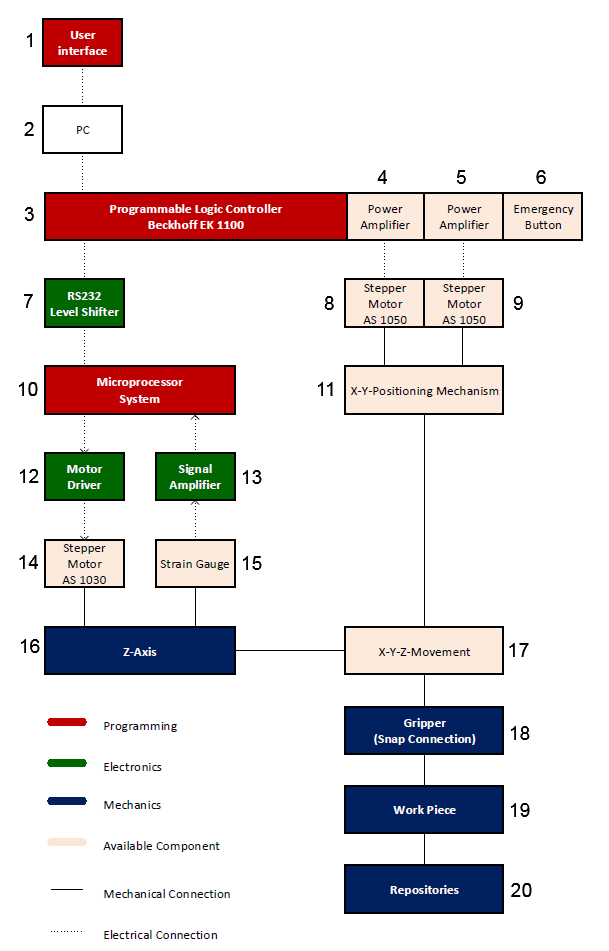
\includegraphics[width=0.8\textwidth]{pictures/SystemDesign}
   \caption[System overview]{System overview\\
	Source: ilias
  }
   \label{fig:system overview}
\end{figure} 





\chapter{Mechanical Components}

\section{\acs{Repository}}\label{sec:repository}

We need an apparatus to grab and release a disc. There are some functions or characteristics that it must perform. First, it is used as a holder to fix the disc with a hole. Second, it needs enough space for moving a snap connector and z-axis. Third, it should be strongly fixed to the floor of a manipulator. Last, it should be better if a structure and assembly are easier. Considering these points, we designed a unique type of an apparatus for a \acs{Repository}.\\
These are isometric (\autoref{fig:repository_1}) and front view (\autoref{fig:repository_2}) of the apparatus. We can easily grab and release the disc by sliding in to the long hole of the plates. All we needed to manufacture were two plates because we use bolts and nuts which already exists.
  \begin{figure}[H]
        \centering
        \begin{subfigure}[b]{0.45\textwidth}
                \centering
                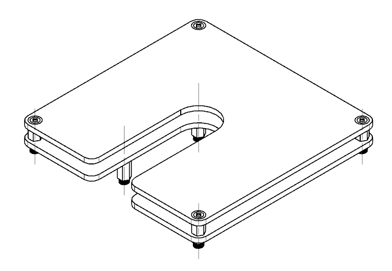
\includegraphics[width=1\textwidth]{pictures/repository_1}
                \caption{Side View}\label{fig:repository_1}
        \end{subfigure}%
        ~ % An dieser Stelle kann ein zusätzlicher Zwischenraum eingebunden werden: ~, \quad, \qquad, \hfill usw.
          % Eine leere Zeile erzwingt, dass die zweite Grafik darunter erscheint.
        \begin{subfigure}[b]{0.45\textwidth}
                \centering
                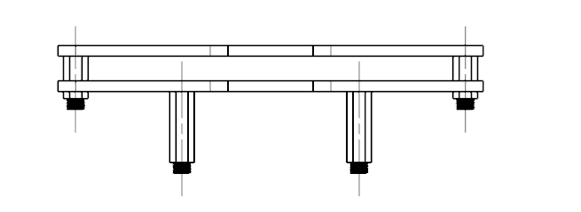
\includegraphics[width=1\textwidth]{pictures/repository_2}
                \caption{Front view}\label{fig:repository_2}
        \end{subfigure}
        \caption[Complete assembly]{Complete assembly}\label{fig:repository_1_2}
  \end{figure}


There are four simple holes with the diameter of 5 mm on the upper steel plate to fix it to the lower plate (\autoref{fig:repository_3}).

And there are eight simple holes whose holes are also 5mm wide to fix it to the upper plate as well as the floor of the manipulator (\autoref{fig:repository_4}).
  \begin{figure} [H]
        \centering
        \begin{subfigure}[b]{0.45\textwidth}
                \centering
                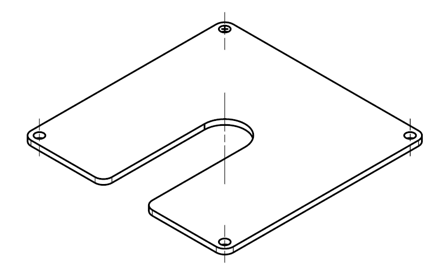
\includegraphics[width=1\textwidth]{pictures/repository_3}
                \caption{Top}\label{fig:repository_3}
        \end{subfigure}%
        ~ % An dieser Stelle kann ein zusätzlicher Zwischenraum eingebunden werden: ~, \quad, \qquad, \hfill usw.
          % Eine leere Zeile erzwingt, dass die zweite Grafik darunter erscheint.
        \begin{subfigure}[b]{0.45\textwidth}
                \centering
                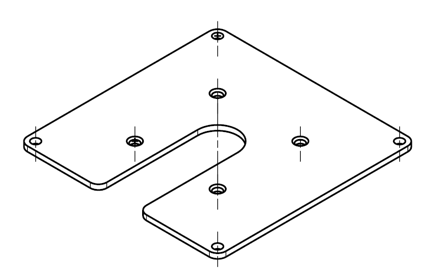
\includegraphics[width=1\textwidth]{pictures/repository_4}
                \caption{Bottom}\label{fig:repository_4}
        \end{subfigure}
        \caption[Top and bottom plate]{Top and bottom plate}\label{fig:repository_3_4}
  \end{figure}

\section{Z-Axis}


\subsection{Frame}
Frame fix the other parts in to the X, Y axes. It has 12 holes in total from where 4 are diameter of $6mm$ and others diameter of $7mm$. Bigger holes are used to fix frame to the axes. Others are to fix linear axis and motorholder to the plate. By using this plate we were able to use motorholder part which was possible to manufacture in school.

  \begin{figure} [H]
        \centering
        \begin{subfigure}[b]{0.55\textwidth}
                \centering
                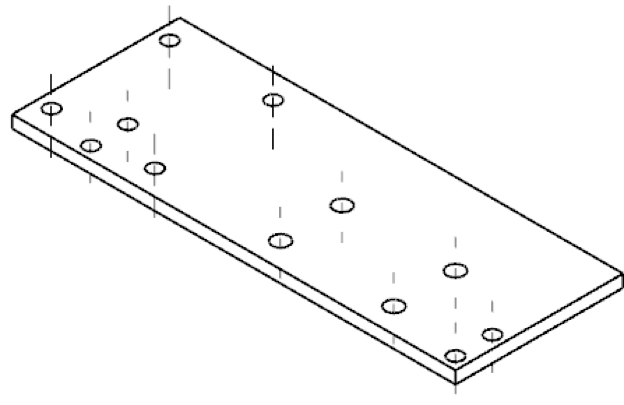
\includegraphics[width=1\textwidth]{pictures/frame_1}
                \caption{side view}\label{fig:frame side view}
        \end{subfigure}%
        ~ % An dieser Stelle kann ein zusätzlicher Zwischenraum eingebunden werden: ~, \quad, \qquad, \hfill usw.
          % Eine leere Zeile erzwingt, dass die zweite Grafik darunter erscheint.
        \begin{subfigure}[b]{0.35\textwidth}
                \centering
                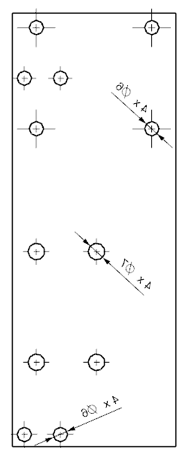
\includegraphics[width=0.5\textwidth]{pictures/frame_2}
                \caption{top view}\label{fig:frame top view}
        \end{subfigure}
        \caption[Frame side and top view]{Frame side and top view}\label{fig:side and top view}
  \end{figure}

\subsection{Mounters for linear Axis and Limit Switch}
The main function of the mounter linear axis to a certain distance. Using designed L-shaped mounters we were able to have linear axis at its desired place. Secondly we designed these to have places to attach a limit switch as well. The limit switch is placed to side of linear axis to minimize the stress and also protect it in a case of malfunction. There are places for two limit switches, one for each mounter at the top and the down of linear axis. We are only using a limit switch at the top one. The down one is in reserve. 
  \begin{figure} [H]
        \centering
        \begin{subfigure}[b]{0.45\textwidth}
                \centering
                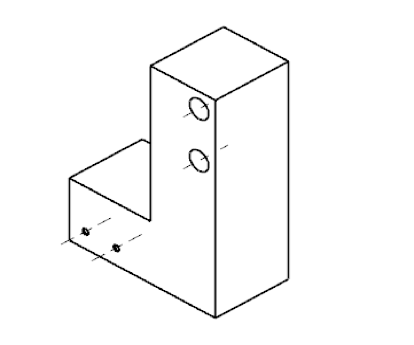
\includegraphics[width=1.3\textwidth]{pictures/linear_axis_1}
                \caption{side view}\label{fig:linear_axis_1}
        \end{subfigure}%
        ~ % An dieser Stelle kann ein zusätzlicher Zwischenraum eingebunden werden: ~, \quad, \qquad, \hfill usw.
          % Eine leere Zeile erzwingt, dass die zweite Grafik darunter erscheint.
        \begin{subfigure}[b]{0.45\textwidth}
                \centering
                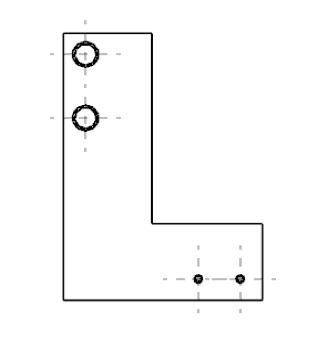
\includegraphics[width=1\textwidth]{pictures/linear_axis_2}
                \caption{front view}\label{fig:linear_axis_2}
        \end{subfigure}
        \caption[Mounters for linear axis and limit switch]{Mounters for linear axis and limit switch\\
        Source: Group 4}\label{fig:linear_axis_1_2}
  \end{figure}
Mounters have four holes two diameter of $6mm$ holes for fitting it to frame, and two diameter of $2mm$ holes to mount limit switch to it (\autoref{fig:linear_axis_1_2}). 	

\subsection{Mounter for Electrical Boards}\label{sec:Mounter for electrical boards}
The mounter has two similar L-shaped parts. For mounting the electrical boards our goal was to have it as easily detached as possible. That's why we were ended up with the design (\autoref{fig:pcb_mounting}) in which you can attach it by just simply sliding it between the two parts of the mounter.

  \begin{figure} [H]
        \centering
        \begin{subfigure}[b]{0.45\textwidth}
                \centering
                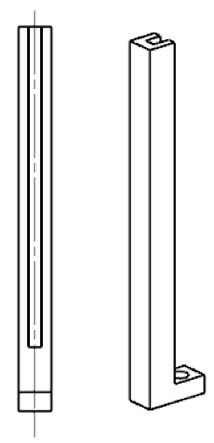
\includegraphics[width=0.45\textwidth]{pictures/pcb_mounting_1}
                \caption{Side view}\label{fig:pcb_mounting_2}
        \end{subfigure}%
                \begin{subfigure}[b]{0.45\textwidth}
                \centering
                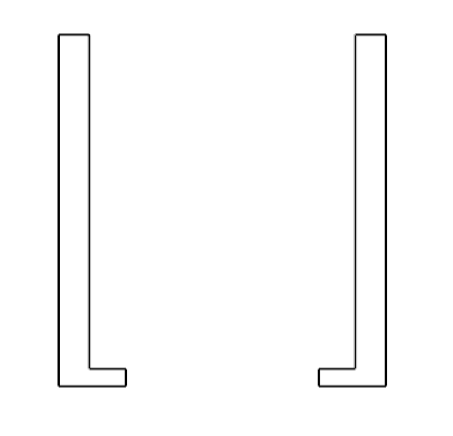
\includegraphics[width=1\textwidth]{pictures/pcb_mounting_3}
                \caption{Front view}\label{fig:pcb_mounting_3}
        \end{subfigure}
        \caption[Mounting for the \acs{PCB}]{Mounting for the \acs{PCB}\\
        Source: Group 4}\label{fig:pcb_mounting}
  \end{figure}     
  
 \subsection{Rackbar}

This part is placed on the carriage of the linear axis. On this part is the strain gauge fixed. This part is fixed with four holes of diameter $3mm$ to the linear axis. The other hole (diameter $5mm$) is to fix the strain gauge. In \autoref{fig:rackbar} the part is shown.

 \begin{figure}[H]
  \centering
   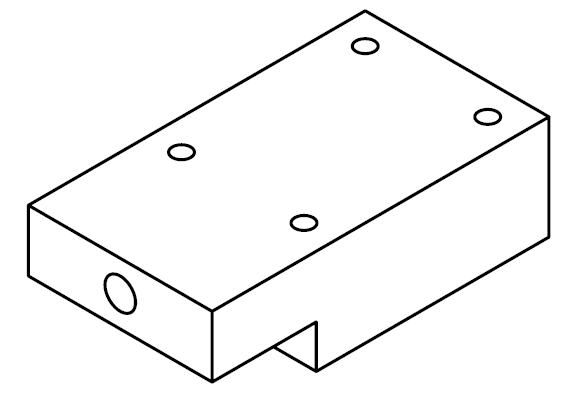
\includegraphics[width=0.5\textwidth]{pictures/rackbar_5}
   \caption[Rackbar]{Rackbar\\
	Source: Group 4  
  }
   \label{fig:rackbar}
\end{figure} 

All of those five holes are clearance holes to provide connection through the body of this part. The thickness of this part is important because if the part is to thin there will be a collision between the snapper and the linear axis. The thickness of $17mm$ guarantees, that the snapper won't hit the axis at any time.

\subsection{Motor Frame}
This part has several tasks to fulfil. The main function is to fix the stepper motor. In addition to this the holding elements for the \acs{uC} are attached to this part. \autoref{fig:motor frame side view} shows the holes which are used to fix the motor. 

  \begin{figure} [H]
        \centering
        \begin{subfigure}[b]{0.45\textwidth}
                \centering
                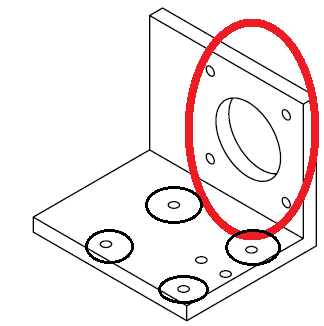
\includegraphics[width=0.8\textwidth]{pictures/frame1_2_2}
                \caption{side view}\label{fig:motor frame side view}
        \end{subfigure}%
        ~ % An dieser Stelle kann ein zusätzlicher Zwischenraum eingebunden werden: ~, \quad, \qquad, \hfill usw.
          % Eine leere Zeile erzwingt, dass die zweite Grafik darunter erscheint.
        \begin{subfigure}[b]{0.45\textwidth}
                \centering
                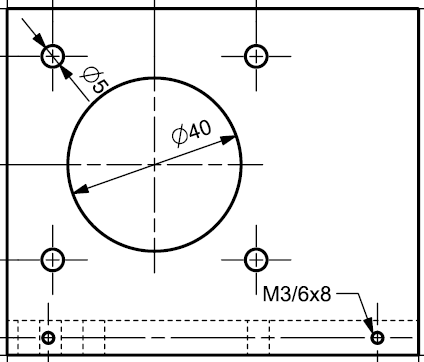
\includegraphics[width=1\textwidth]{pictures/frame1_5}
                \caption{front view}\label{fig:motor frame front view}
        \end{subfigure}
        \caption[Motor frame]{Motor frame\\
        Source: Group 4}\label{fig:motor frame}
  \end{figure}

This part is fixed to the baseplate with four holes. Those 4 holes are marked with four black ellipsis in \autoref{fig:motor frame side view} above. To fulfil the fixation of the \acs{uC} there are two additional holes in this plate. This holes are used to fix the parts that are necessary to hold the \acs{uC} board. This holes can be seen in \autoref{fig:motor frame front view} above.

 
There are two threaded holes (M3) to attach the \acs{uC} fixation. The \acs{uC} fixation parts are described in \autoref{sec:Mounter for electrical boards}.

\section{Mechanical Assembly}
In \autoref{fig:mechanical assembly} is the assembled construction shown and in \autoref{tab:parts lists} are the corresponding single parts shown with the quantity.
 \begin{figure}[H]
  \centering
   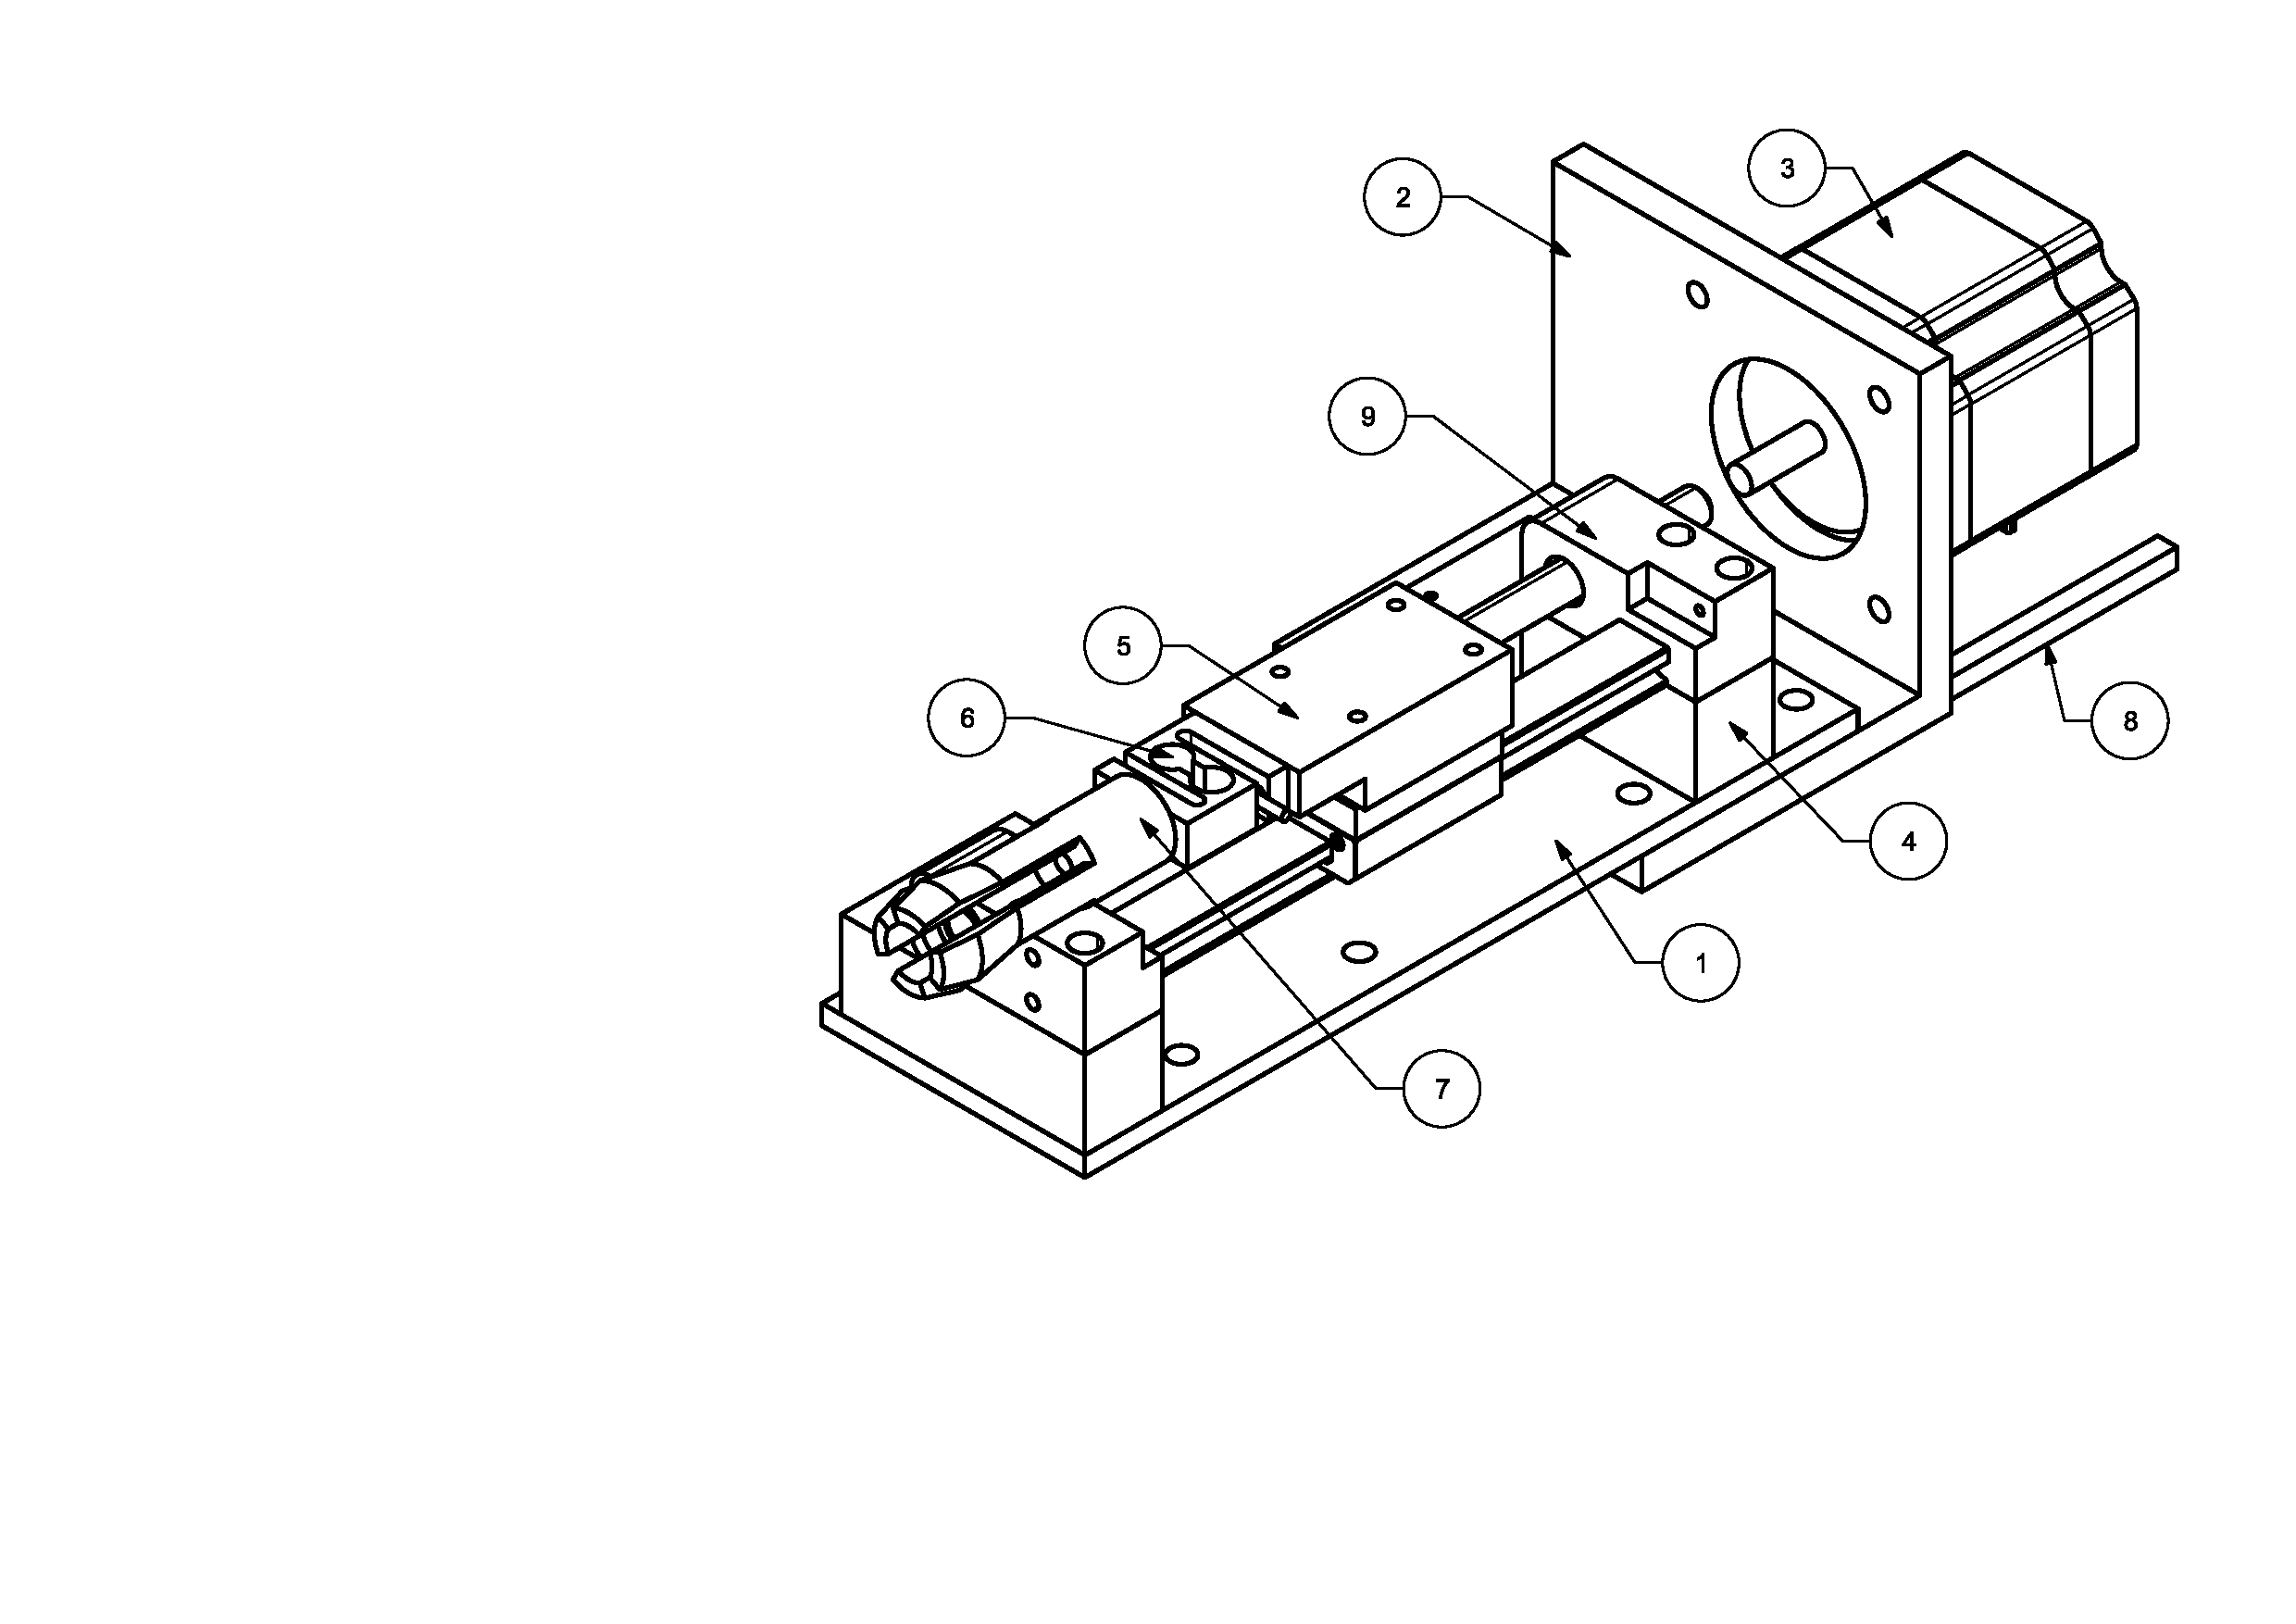
\includegraphics[width=1\textwidth]{pictures/psi5321_asseblyAxisGes}
   \caption[Mechanical assembly]{Mechanical assembly\\
	Source: Group 4  
  }
   \label{fig:mechanical assembly}
\end{figure} 

\begin{table}[H]
\centering
\begin{tabular}{|l|l|l|}
\hline
Number & Name                & Quantity \\ \hline
1      & Baseplate           & 1        \\ \hline
2      & Motorholder         & 1        \\ \hline
3      & Motor               & 1        \\ \hline
4      & Linear axis fitting & 2        \\ \hline
5      & Rackbar             & 1        \\ \hline
6      & Strain gauge        & 1        \\ \hline
7      & Snap connection     & 1        \\ \hline
8      & Microfix            & 2        \\ \hline
9      & Linear axis 100m    & 1        \\ \hline
\end{tabular}
\caption{Parts lists}
\label{tab:Parts lists}
\end{table}
     
\section{Snap Connection}

For grabbing the object (disc) there is a grabber needed. For this task the best and easiest solution is a snap connection. With the snapper it is possible to grab the disc and you can also drop it with a special construction. This construction is called \acs{Repository} and is described in \autoref{sec:repository}. The force which is needed to get through the hole of the disc is measured with a strain gauge (\autoref{sec: amplifier circuit}) This strain gauge has a measuring range of $+/- 10N$. For designing the snap connection this means that the maximum force must not exceed $+10N$ and the same is for the force which is needed to get out of the hole. Otherwise the force will be out of range and this means that the force can't be measured. In the following figure there is the design of the snap connector.

 \begin{figure}[H]
  \centering
   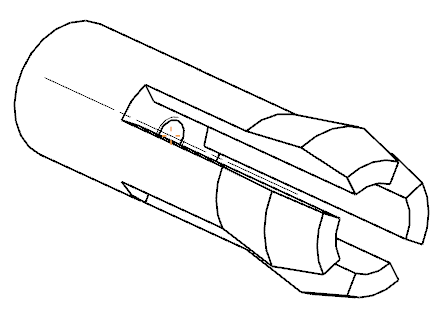
\includegraphics[width=0.5\textwidth]{pictures/Snap1}
   \caption[Snap connector]{Snap connector\\
	Source: Group 4  
  }
   \label{fig:snap connector}
\end{figure} 

The snap connector has four arms. The length of each arm is $40mm$ and the thickness is $3mm$. This thickness guarantees a certain stiffness of the snapper. The snapper has to be that stiff that the disc with a weight of approximately $100g$ ($1N$) can't drop itself just because of its weight.

\subsection{Calculation of the Forces}
To guarantee that the forces are within the range of the gauge, the forces of the snap connector has to be calculated. The calculation is simplified by assuming the circle-section form to a rectangular form. Because the shape of the circle-section is nearly the same than the shape of the rectangular. So the difference in the calculation is not that big. The diameter of the hole in the disc is $20mm$. The outer diameter of the designed snapper is $22mm$. This means that each arm of the snap connector needs to be displaced at least 1 mm. There are two different forces. One for pushing the snapper through the hole of the disc and the second one is the force for pulling the snapper out of the hole.

\subsubsection{Calculation of the Force for Grab Cycle}

The following values are given for the calculation:
\begin{itemize}
\item $f = 1 mm$ (displacement)
\item $b = 7 mm$ (width of the finger)
\item $h = 3 mm$ (thickness of the wall)
\item $\mu = 0,5$ (friction factor; Plastic on Metal)
\item $\alpha = 14,03^{\circ}$ (angle of the snapper)
\item $l = 40 mm$ (length of the arm)
\item As material for the simulation was chosen  ABS
\item $ES = 2500 N/mm^{2}$ (ABS)
\end{itemize}
With the needed displacement of each arm of about $1mm$ the following equation leads to the shear force. Out of the \autoref{eq:displacement the strain} for the displacement the strain can be calculated.

\begin{eqnarray}
f &=& \frac{2}{3}*\frac{\varepsilon*l^{2}}{h}\label{eq:displacement the strain}\\
\rightarrow \varepsilon &=& \frac{3*f*h}{2*l^{2}}\\
\varepsilon  &=& \frac{3*1mm*3mm}{2*(40mm)^{2}} = 0.0028
\end{eqnarray}

With the result of the strain the shear force can be calculated. But for the calculation of the shear force ($Q$), the section modulus ($W$) is needed. The following equation shows how the section modulus is calculated.

\begin{eqnarray}
W &=& \frac{b*h^{2}}{6}\\
W &=& \frac{7mm*(3mm)^{2}}{6} = 10.5 mm^{3}
\end{eqnarray}

Now all values which are necessary for the calculation of the shear force are known. 

\begin{eqnarray}
Q &=& W*\frac{E_{S}*\varepsilon}{l}\\
Q &=& 10.5mm^{3}* \frac{2500\frac{N}{mm^{2}}*0.0028}{40 mm} = 1.8375 N
\end{eqnarray}

The axial force can be calculated out of the shear force with the angle of the snapper. The following equation shows how to calculate this force.

\begin{eqnarray}
F &=& Q*\frac{\mu + \tan (\alpha)}{1 - \mu * \tan (\alpha)}\\
F &=& 1.8375N*\frac{0.5 + \tan(14.03)}{1 - 0.5 * \tan(14.03)} = 1.575 N
\end{eqnarray}

This means with a force of $1.575 N$ one arm of the snap connection displaces about $1mm$. For each arm is the same force needed. This means that the whole force for the four arms is calculated as follows:

\begin{eqnarray}
F_{tot} &=& 4 * F \\
F_{tot}  &=& 4 * 1.575N = 6.298 N
\end{eqnarray}
The calculated total force is within the range of the strain gauge.

\subsubsection{Calculation for the Drop Cycle}

The values for this calculation are almost the same. Just the length changes from $40mm$ to $32mm$ and the angle is now $9.46^{\circ}$.
\begin{itemize}
\item $f = 1 mm$ (displacement)
\item $b = 7 mm$ (width of the finger)
\item $h = 3 mm$ (thickness of the wall)
\item $ \mu = 0.5$ (friction factor; Plastic on Metal)
\item $ \alpha = 9.46^{\circ}$ (angle of the snapper)
\item $l = 32 mm$ (length of the arm)
\item As material for the simulation was chosen  ABS
\item $ES = 2500 N/mm^{2}$ (ABS)
\end{itemize}

The equations are the same than before. Just the values for the length of an arm and the angle are different.

\begin{eqnarray}
f &=& \frac{2}{3}*\frac{\varepsilon*l^{2}}{h}\\
\rightarrow \varepsilon &=& \frac{3*f*h}{2*l^{2}}\\
\varepsilon &=& \frac{3*1mm*3mm}{2*(32mm)^{2}} = 0.0044
\end{eqnarray}

The calculation for the section modulus is exactly the same than in the point above.

\begin{eqnarray}
W &=& \frac{b*h^{2}}{6}\\
W &=& \frac{7mm*(3mm)^{2}}{6} = 10.5 mm^{3}
\end{eqnarray}

\begin{eqnarray}
Q &=& W*\frac{E_{S}*\varepsilon}{l}\\ 
Q &=& 10.5mm^{3}* \frac{2500\frac{N}{mm^{2}}*0.0044}{32 mm} = 2.8839 N
\end{eqnarray}

\begin{eqnarray}
F &=& Q*\frac{\mu + \tan (\alpha)}{1 - \mu * \tan (\alpha)}\\
F &=& 2.8839*\frac{0.5 + \tan(14.03)}{1 - 0.5 * \tan(14.03)} = 2.097 N
\end{eqnarray}

\begin{eqnarray}
F_{ges} &=& 4 * F\\
F_{ges} &=& 4 * 2.097N = 8.389 N
\end{eqnarray}

The total force is now $8.389N$ and this means that the force is within the range of the gauge.

\subsection{\acs{FEA}}

With the finite element analysis it's possible to show and to check the occurring stresses and displacements. The \acs{FEA} was made with the program NX 10. The first step for this simulation was to split the whole object into small elements. The elements are tetrahedron elements. \autoref{fig:dividing into a finite number of elements} shows how the object looks like when it's divided into a finite number of elements.

 \begin{figure}[H]
  \centering
   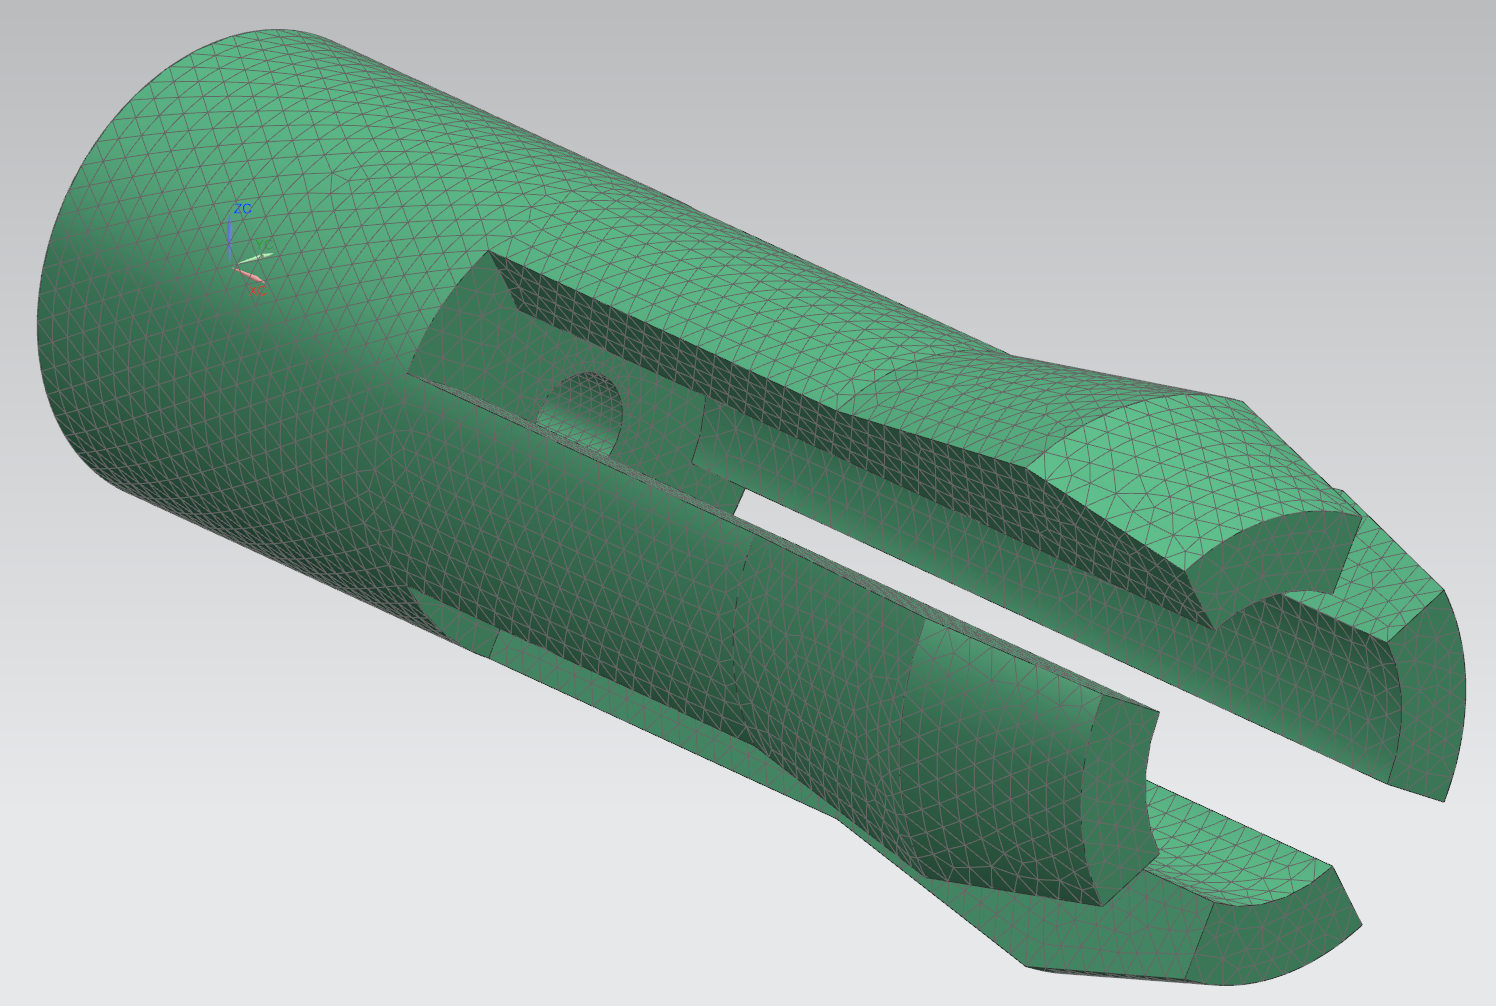
\includegraphics[width=1\textwidth]{pictures/FEA1}
   \caption[Dividing into a finite number of elements]{Dividing into a finite number of elements\\
	Source: Group 4  
  }
   \label{fig:dividing into a finite number of elements}
\end{figure} 

The bending behaviour of different materials is different, so a material has to be defined that behaviour is acceptable. The chosen material for the simulation was ABS because it is a good material for bending tasks. The next point was to define where the snapper is fixed and where the loads are acting. As seen in \autoref{fig:attached object  and loads} there is shown where the object is attached and where the loads act.

 \begin{figure}[H]
  \centering
   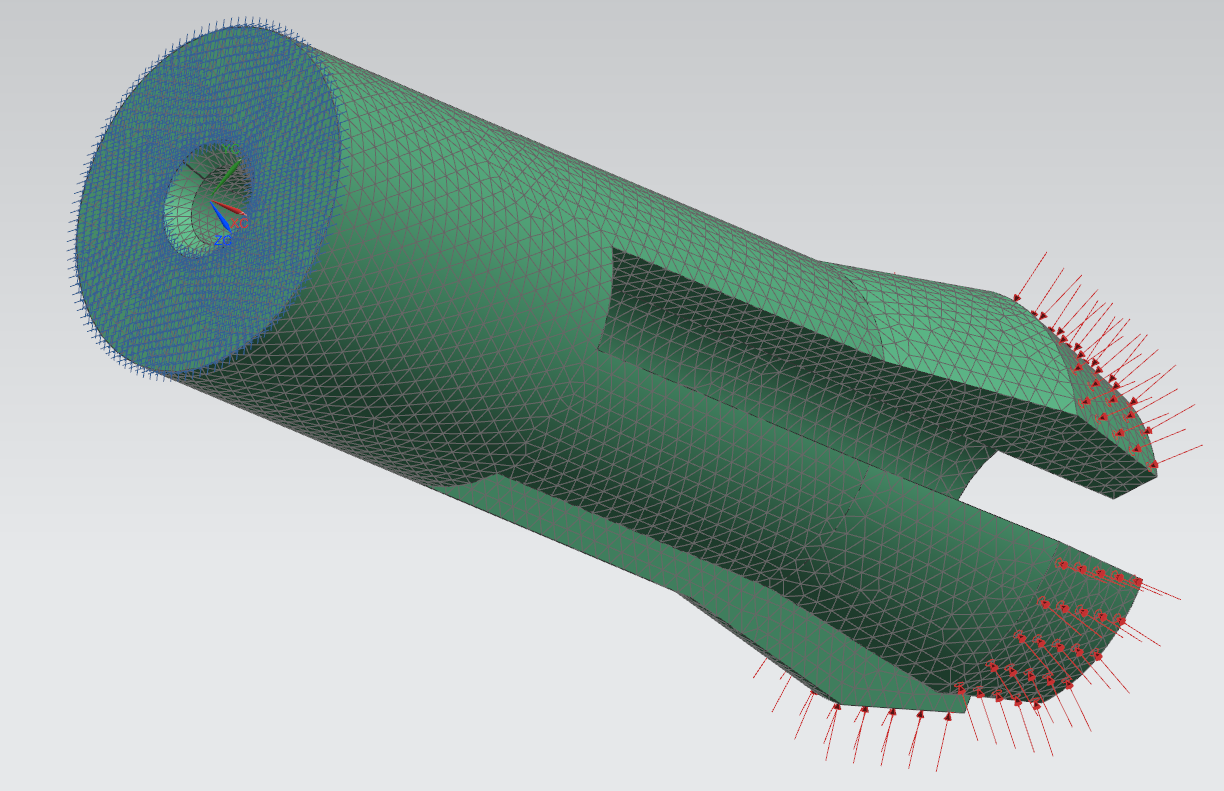
\includegraphics[width=1\textwidth]{pictures/FEA2}
   \caption[Attached object  and loads]{Attached object  and loads\\
	Source: Group 4  
  }
   \label{fig:attached object  and loads}
\end{figure} 

In the figure above you can see that the area where the snapper is fixed is marked blue. The loads are represented by the red arrows acting on four areas. The pressure is calculated as follows. The area where the pressure is acting is about $86.35mm^{2}$ big. The force which is acting on one area is about $2,5N$. The pressure for the simulation is $0.029 N/mm^{2}$. 

\begin{eqnarray}
p &=& \frac{F}{A}\\
p &=& \frac{2.5N}{86.35 mm^{2}} = 0.0289 \frac{N}{mm^{2}}
\end{eqnarray}

\subsection{Analysis of the Simulation for the Displacement}
The snapper has to be deformed at least one mm at each arm that the snapper is able to snap into the disc. In \autoref{fig:displaced snapper} is the displaced snapper shown. 

 \begin{figure}[H]
  \centering
   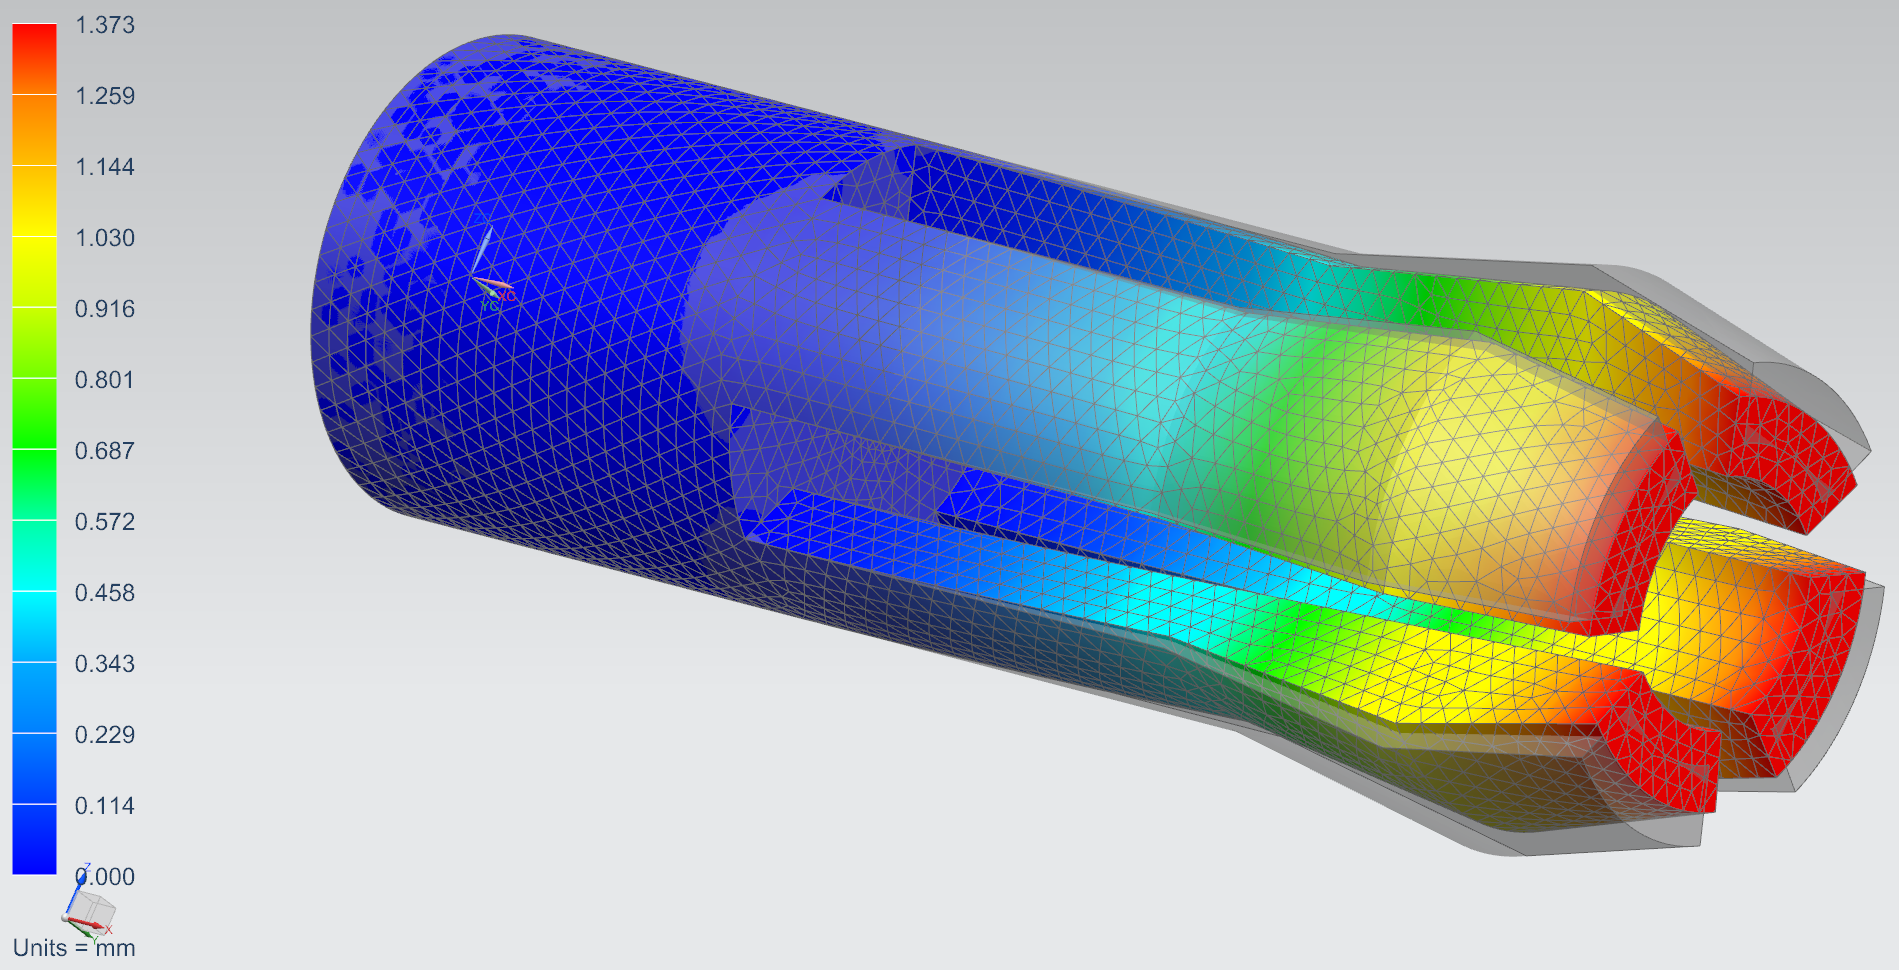
\includegraphics[width=1\textwidth]{pictures/FEA4}
   \caption[Displaced snapper]{Displaced snapper\\
	Source: Group 4  
  }
   \label{fig:displaced snapper}
\end{figure}

The colours stands for different displacements. The scale on the left side in the picture shows which colour stands for which displacement value. At the yellow region the displacement is bigger than 1mm. The yellow region is the important region because the edge there should be deformed at least 1mm. The used material for manufacturing is Polyamide. The ABS was chosen for calculation because this two materials are really similar. The Polyamide is the softer material, so the displacement will be bigger for the same force or the force to displace the snapper for the same distance will be a little smaller.

\subsection{Analysis of the Simulation for the Stresses}
The simulation result for the stresses looks similar to the simulation result of the displacement. The scale on the left side shows the stress and the colours shows the location of the acting stresses. \autoref{fig:simulation result} shows the result of the simulation.
 \begin{figure}[H]
  \centering
   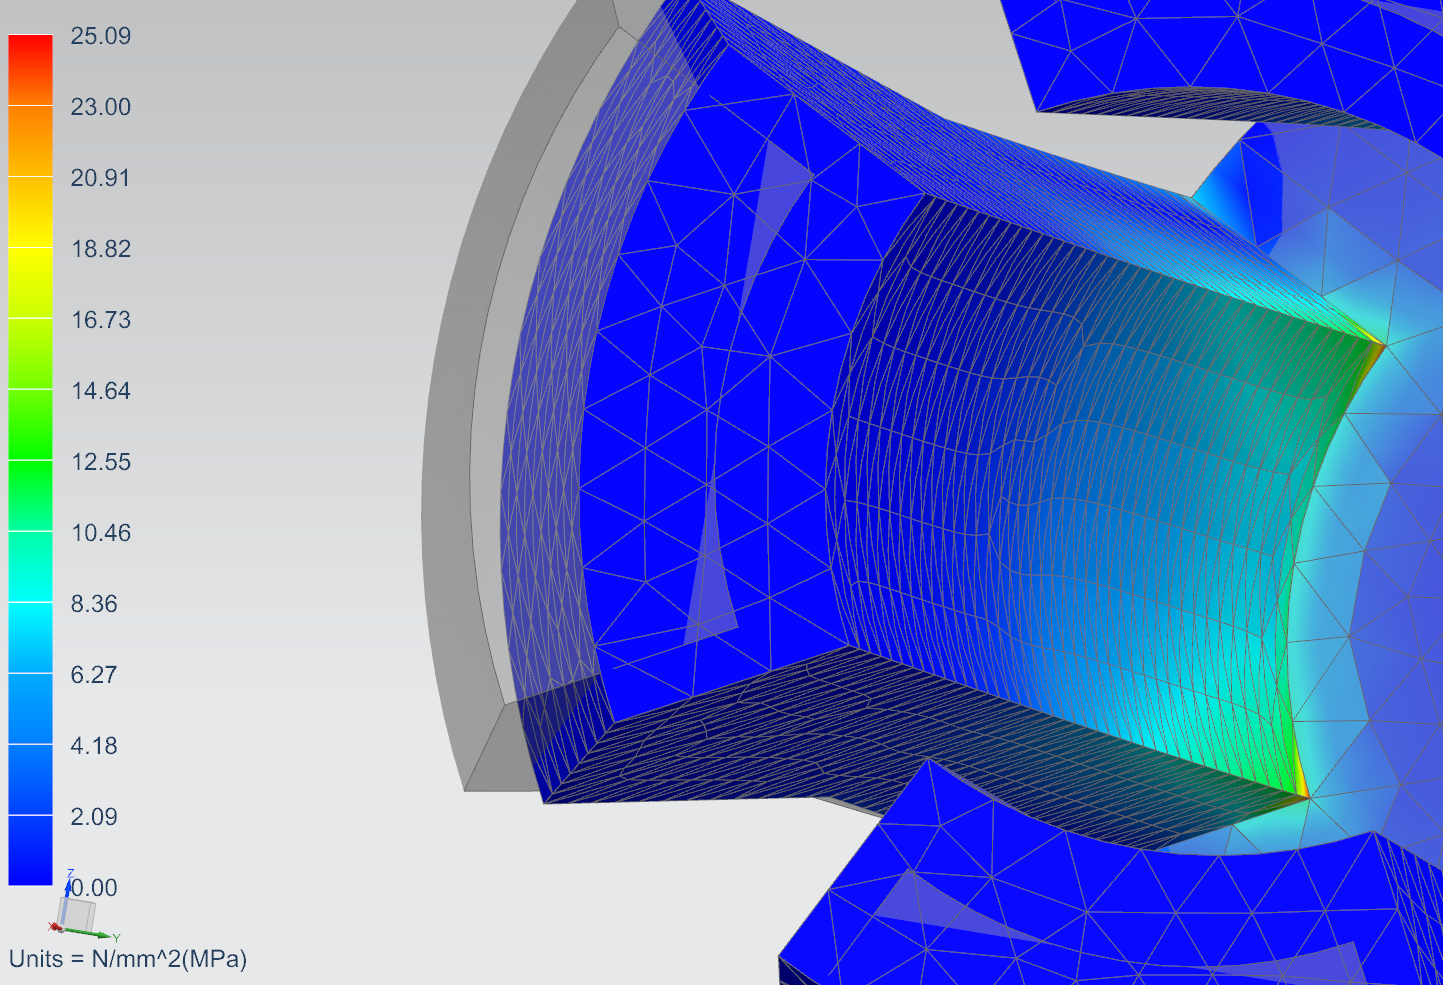
\includegraphics[width=1\textwidth]{pictures/FEA5}
   \caption[Simulation result]{Simulation result\\
	Source: Group 4  
  }
   \label{fig:simulation result}
\end{figure}

The maximum stress occurs at the corners as seen in figure above. The value of the maximum stress is $25.09 N/mm^{2}$.

\chapter{Electronic Components}

\section{System Overview}
\autoref{fig:electronic System Overview} shows the parts that are connected together and which interface is used. The parts will be discussed in this chapter.
 \begin{figure}[H]
  \centering
   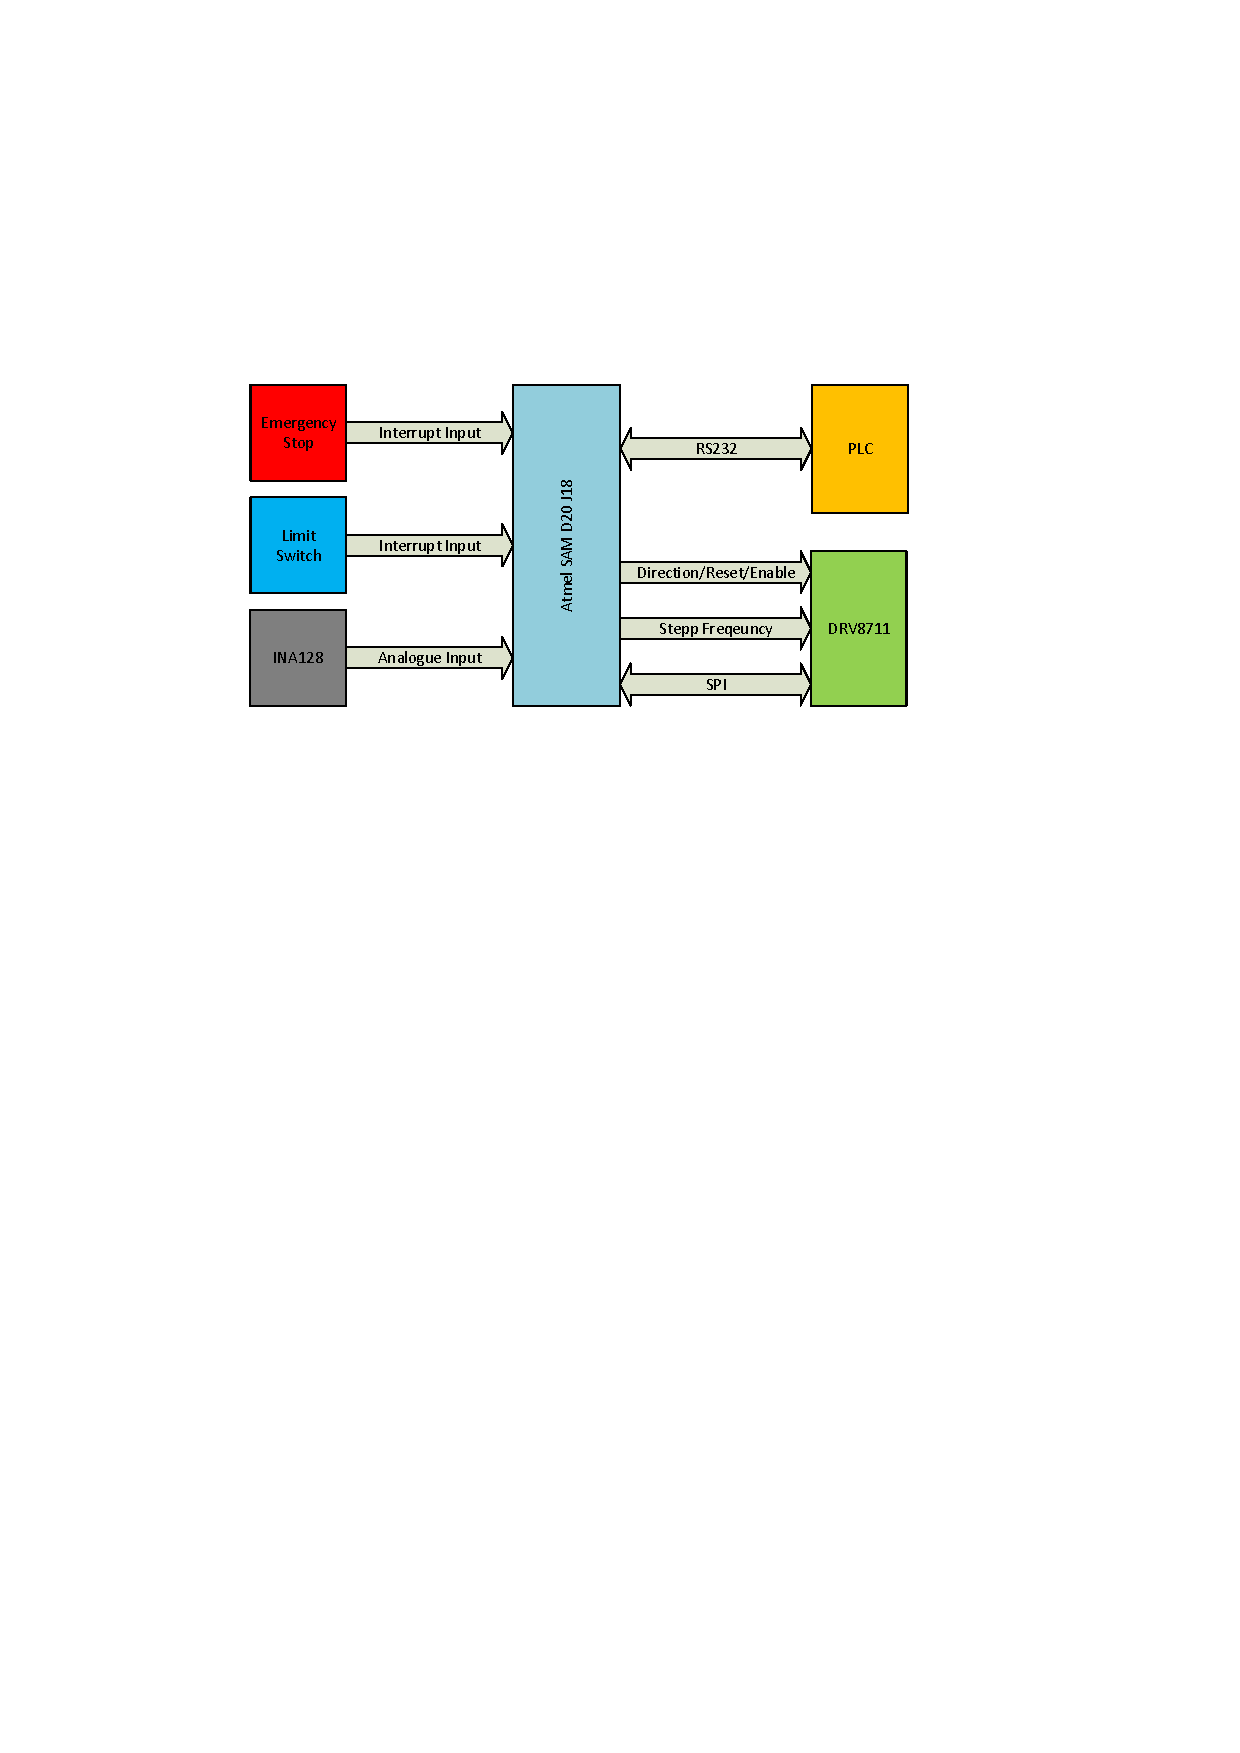
\includegraphics[width=1\textwidth]{pictures/Electronic_overview.pdf}
   \caption[System Overview]{System Overview\\
	Source: Group 4}
     \label{fig:electronic System Overview}
\end{figure}

\section{Linear Voltage Regulator}
The linear voltage regulator is primarily to supply the amplifier with a constant voltage, but the $5V$ are also used for the \acs{uC} and the \acs{RS232} level converter. A \enquote{LM1086} is used, because it satisfies the needs for our schematic and it is in stock at the FHV.

\section{Schematic}

In the left top corner in \autoref{fig:scematic_power_rs232_strain.pdf} the linear voltage regulator can be found. There are two capacitors (C13, C14) for bypassing\footnote{the values are chosen from the \enquote{LM1086} data sheet page 18}

\section{Calculation}

The maximum current has to be calculated, because if the current is to high, a heat sink has to be used.
With the following equation it leads us to the maximum current.
\begin{eqnarray}
P_{D}=(V_{in}-V_{out})*I_{L}
\end{eqnarray}
$P_{D}...power \, consumption$\\
$I_{L}...load \, current$
\begin{eqnarray}
R_{therm} &=& \frac{T_{j}-T_{a}}{P_{D}}\\
R_{therm} &=&  \frac{T_{j}-T_{a}}{(V_{in}-V_{out})*I_{L}}
\end{eqnarray}
$T_{j}...junction \, temperature$\\
$T_{a}...ambient \, temperature$
With the following values\footnote{they can be found in the \enquote{LM1086} data sheet at page 4 and 5}, the maximum current can be calculated.
$T_{j}=125^{\circ}$
$T_{a}=25^{\circ}$
$R_{therm}=40,8^{\circ}C/W$
\begin{eqnarray}
\rightarrow I_{L} &=&  \frac{T_{j}-T_{a}}{(V_{in}-V_{out})*R_{therm}}\\
I_{L} &=&  \frac{125^{\circ}C-25^{\circ}C}{24V-5V)*40,8^{\circ}C/W}=0,129A\label{eq:result max current LM1086}
\end{eqnarray}
The result of \autoref{eq:result max current LM1086} is higher then the the measurements in \autoref{sec: measurements LM1086}. Consequently no heat sink is needed.

\section{Measurements}\label{sec: measurements LM1086}
The current and the voltage is measured under load. Current was about $50mA$ and the voltage constant at $5V$.

\section{Amplifier Circuit}\label{sec: amplifier circuit}
\subsection{Description}
The main purpose of the circuit (\autoref{fig:scematic_power_rs232_strain.pdf}) is to amplify the differential voltage between the positive and negative bridge input from the strain gauge. This amplified differential voltage then is send to the \acs{ADC} converter that is located on the Atmel board. The board is operating on a 5V supply voltage and with a reference voltage of $1,65V$. The amplification factor is $660$ (\autoref{eq: Rg calculation}), which is explained later in the document. 

\subsection{Schematic}
On the right side image (\autoref{fig:scematic_power_rs232_strain.pdf}) the schematic for the amplifier can be found. The circuit for the amplifier is connected to the \acs{RS232} and the linear voltage regulator. This because the \acs{RS232} and the amplifier use the same 5V supply voltage that the linear voltage regulator is supplying. The circuit consists of an INA128UA1, a gain resistor (U1), a resistor to adjust the reference voltage (R1) and a capacitor (C5). The values can bee found at \autoref{tab:list of materials}. The amplifier circuit get the positive and negative bridge input from the DMS connector 3 and 4. The amplified output signal is given to the 3th pin of the Atmel board.

\begin{figure}[H]
  \centering
   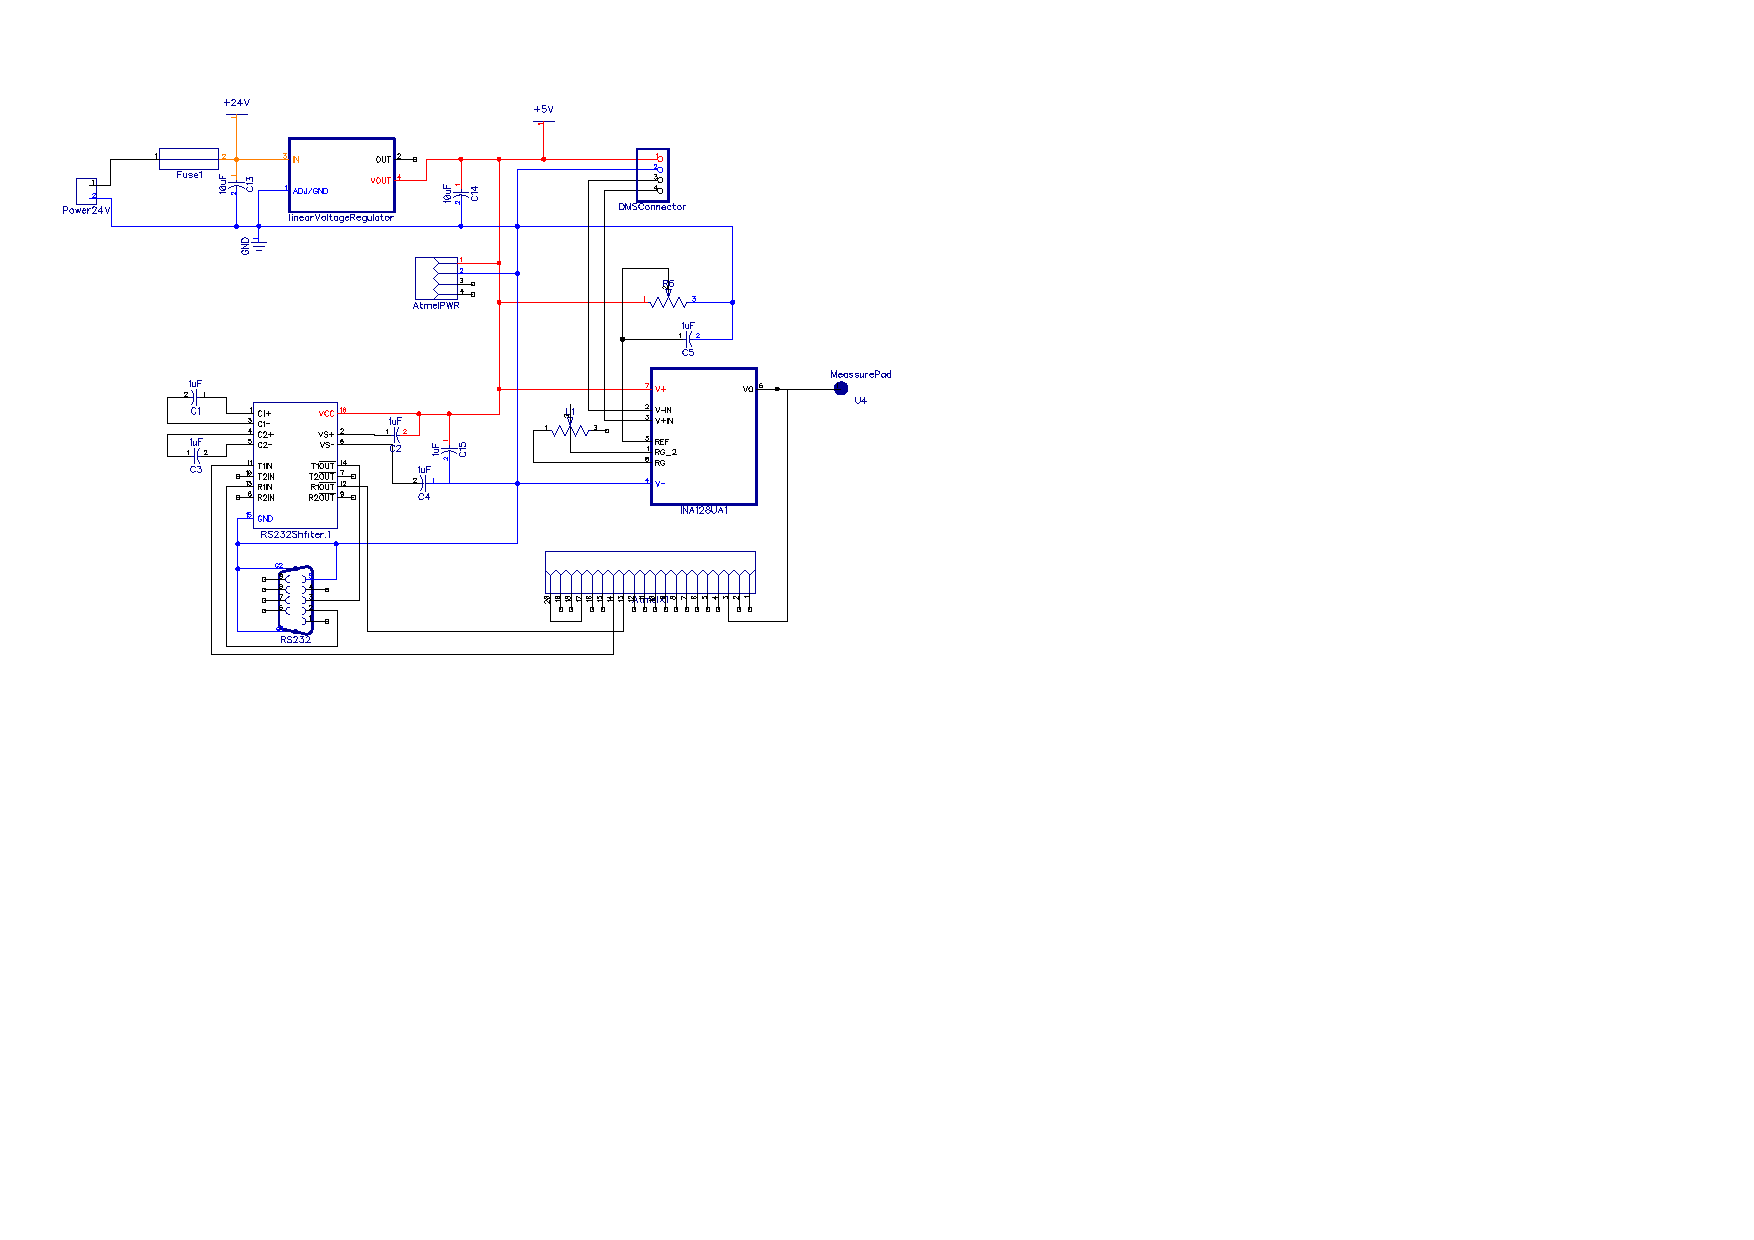
\includegraphics[width=1\textwidth]{pictures/scematic_power_rs232_strain.pdf}
   \caption[Schematic of power, \acs{RS232} and strain gauge]{Schematic of power, \acs{RS232} and strain gauge\\
	Source: Group 4  
  }
   \label{fig:scematic_power_rs232_strain.pdf}
\end{figure} 

\subsection{Calculation}
The following calculation can be found in the datasheet of the INA128UA and is used to calculate the gain of the gain resistor:

With  \autoref{eq: gain generally}  the necessary gain is calculated.

\begin{eqnarray}
G&=&\frac{U_{a}}{U_{e}}\label{eq: gain generally}\\
G&=&\frac{3,3V}{5*10^{-3}V}=660
\end{eqnarray}

The \autoref{eq: gain calculation} is from the IN128UA1 Datasheet.

\begin{eqnarray}
G=1+ \frac{50k \Omega}{R_{g}}\label{eq: gain calculation}
\end{eqnarray}

With \autoref{eq: gain calculation} the $R_{g}$ is calculated.

\begin{eqnarray}
R_{g} =  \frac{50k \Omega}{G-1}\label{eq: Rg calculation}
\end{eqnarray}

With \autoref{eq: Rg calculation} the necessary $R_{g}$ is calculated as $75,8 \Omega$

The reference voltage is calculated with the generally voltage divider formula. The reference voltage should be $1,65V$, because the strain gauge has $0n$ with no load.
\begin{eqnarray}
\frac{U_{2}}{U}&=&\frac{R_{2}}{R_{1}+ R_{2}}\\
\frac{U_{2}}{U}&=&\frac{R_{2}}{R_{ges}}\\
\rightarrow R_{2} &=& \frac{U_{2}*R_{ges}}{U}\\
R_{2} &=& \frac{1,65V*500\Omega}{5V}=165\Omega
\end{eqnarray}
The potentiometer R1 has to be adjusted to $165\Omega$.

\subsection{Layout}
The layout of the top and bottom side of the board is shown in \autoref{fig:PCB layout}.  

\subsection{Measurement}
The measurement is done so there is proof that the amplifier works and so the machine can function well. In \autoref{fig:Strain_gauge_test} the test results can be seen, the sinus shaped line (yellow probe) represents the output voltage that is given to the \acs{ADC}. 

\begin{figure}[H]
  \centering
   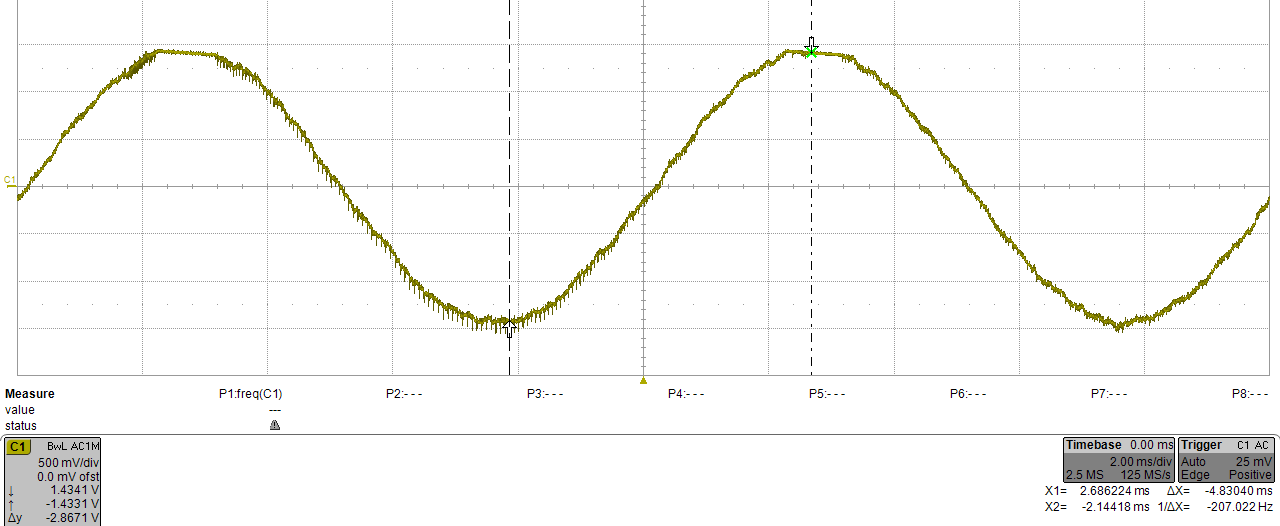
\includegraphics[width=1\textwidth]{pictures/Strain_gauge_test}
   \caption[Test of the strain gauge]{Test of the strain gauge\\
	Source: Group 4  
  }
   \label{fig:Strain_gauge_test}
\end{figure} 

To test the amplifier it is connected to a power supply, a function generator and the oscilloscope. The function generator simulates the positive and negative bridge input, with an offset of 1.675V and a maximum amplitude of 2.5mV.

\section{\acs{RS232} Circuit}
\subsection{Description}
The main purpose of the circuit (\autoref{fig:scematic_power_rs232_strain.pdf}) is to change the \acs{TTL} signal ($0V...3,3V$) to \acs{RS232} ($+15V...-15V$). This is necessary, because the \acs{uC} has only a \acs{TTL} interface  and the \acs{PLC} only a \acs{PLC} interface. And one good thing is, that the \acs{RS232} is stable against disruptions.

\subsection{Schematic}
On the left side image (\autoref{fig:scematic_power_rs232_strain.pdf}) the schematic for the amplifier can be found. The \acs{RS232} circuit is connected to the linear voltage regulator, because the power supply of the  \acs{RS232} is $5V$. The circuit consists of a MAX232, two charge pumps(C1, C3) and three other capacitors (C2, C4, C5). The components were chosen with the guideline of the data sheet, the values can bee found at \autoref{tab:list of materials}. \enquote{R1IN} are the line data input (from \acs{PLC}) and \enquote{T1OUT} the line data output (to \acs{PLC}). \enquote{T1IN} are the logic data input (from \acs{uC}) and \enquote{R1OUT} are logic data output (to \acs{uC}). \enquote{VS+} is the positive charge pump output and \enquote{VS-}  is negative charge pump output.

\subsection{Measurement}
To test the \acs{RS232} it is connected to a power supply, the \acs{uC} and a USB to \acs{RS232} adapter to send and receive data from a computer. First the charge pumps are measured with a voltage meter (values $8V$ and $-6,5V$). Secondly a \acs{ASCII} transmission is send by \acs{uC}. In \autoref{fig:RS232_measurement} is the telegram shown as a scope. In \autoref{fig:RS232_measurement} the yellow probe shows the telegram transmission.

\begin{figure}[H]
  \centering
   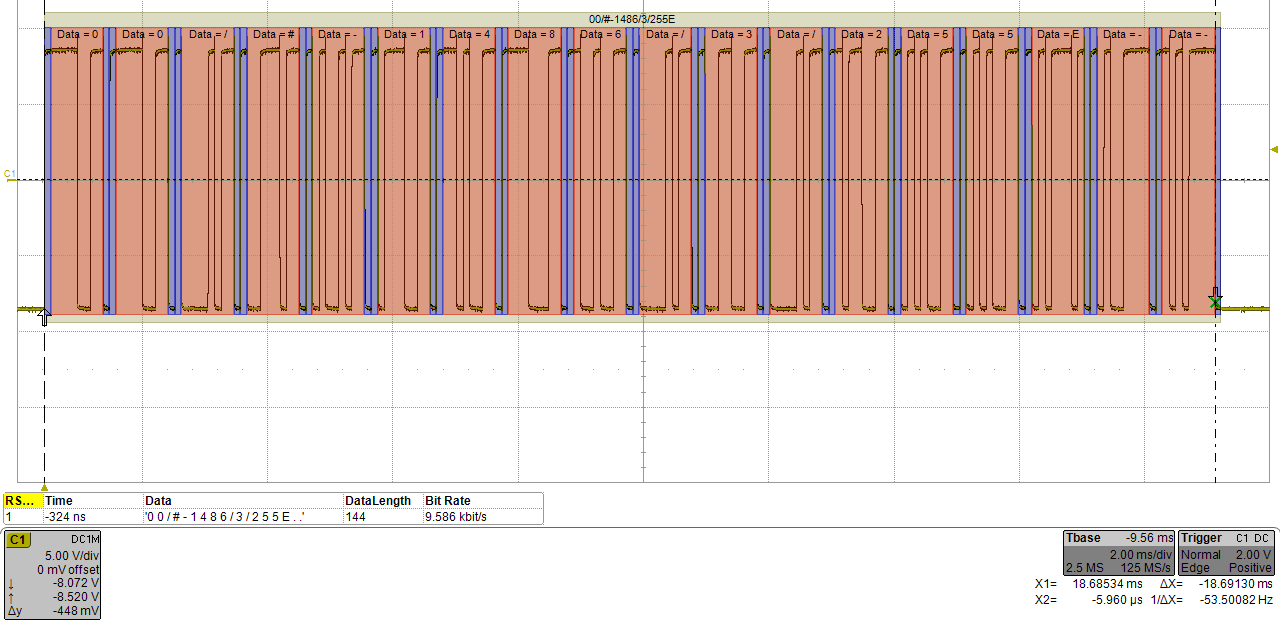
\includegraphics[width=1\textwidth]{pictures/measurements/RS232_measurement}
   \caption[\acs{RS232} telegram scope]{\acs{RS232} telegram scope\\
	Source: Group 4  
  }
   \label{fig:RS232_measurement}
\end{figure} 

As we can see, the telegram is transmitted correctly.

\subsection{Layout}
The layout of the top and bottom side of the board is shown in \autoref{fig:PCB layout}.  


\section{DRV8711 Circuit}
\subsection{Description}
The Z axis of the system is moved by a bipolar stepper motor. To convert low power control signals of any logic device into power signals for the motor a driver circuit had to be implemented. These motor drivers consist basically of a full bridge circuit for each of the both motor windings.

\subsection{Schematic}
A DRV8711 has to be used, so a schematic was designed (\autoref{fig:DRV8711 layout}) to control the stepper motor. The components were chosen with the guideline of the data sheet. Only the IRF520, a N-Channel power \acs{MOSFET}, was chosen, because Mr. Schneider recommend it.\\
The circuits consists of
\begin{itemize}
\item the DRV8711,
\item a charge pump (C8),
\item two resistors (R1, R2) $50 m \Omega$ for the current measurement,
\item two red LED's for stall and error debugging with a dropping resistor (R4, R3) of $220m\Omega$ (see \autoref{sec:calculation_drv8711},
\item two bulk capacitors, one electrolyte (C10) and one ceramic (C11)
\item a pull up resistor for the SDATO (\acs{SPI}), because it's a open-drain output,
\item a bypass to ground (C9) for the $5V$ pin (5)
\item a capacitor(C6) is placed between the \acs{VM} and \acs{VCP},
\item a bypass capacitor (C7) from \acs{VINT} to ground,
\item 8 \acs{MOSFET}'s (T1-T8) for the power section,
\item a plug (motor connector) to connect to the motor,
\item a connector (Atmel X2) with 10x2 pins,
\item two connectors (J1, J2) with each 19 pins
\end{itemize}

\begin{landscape}
\begin{figure}[H]
  \centering
   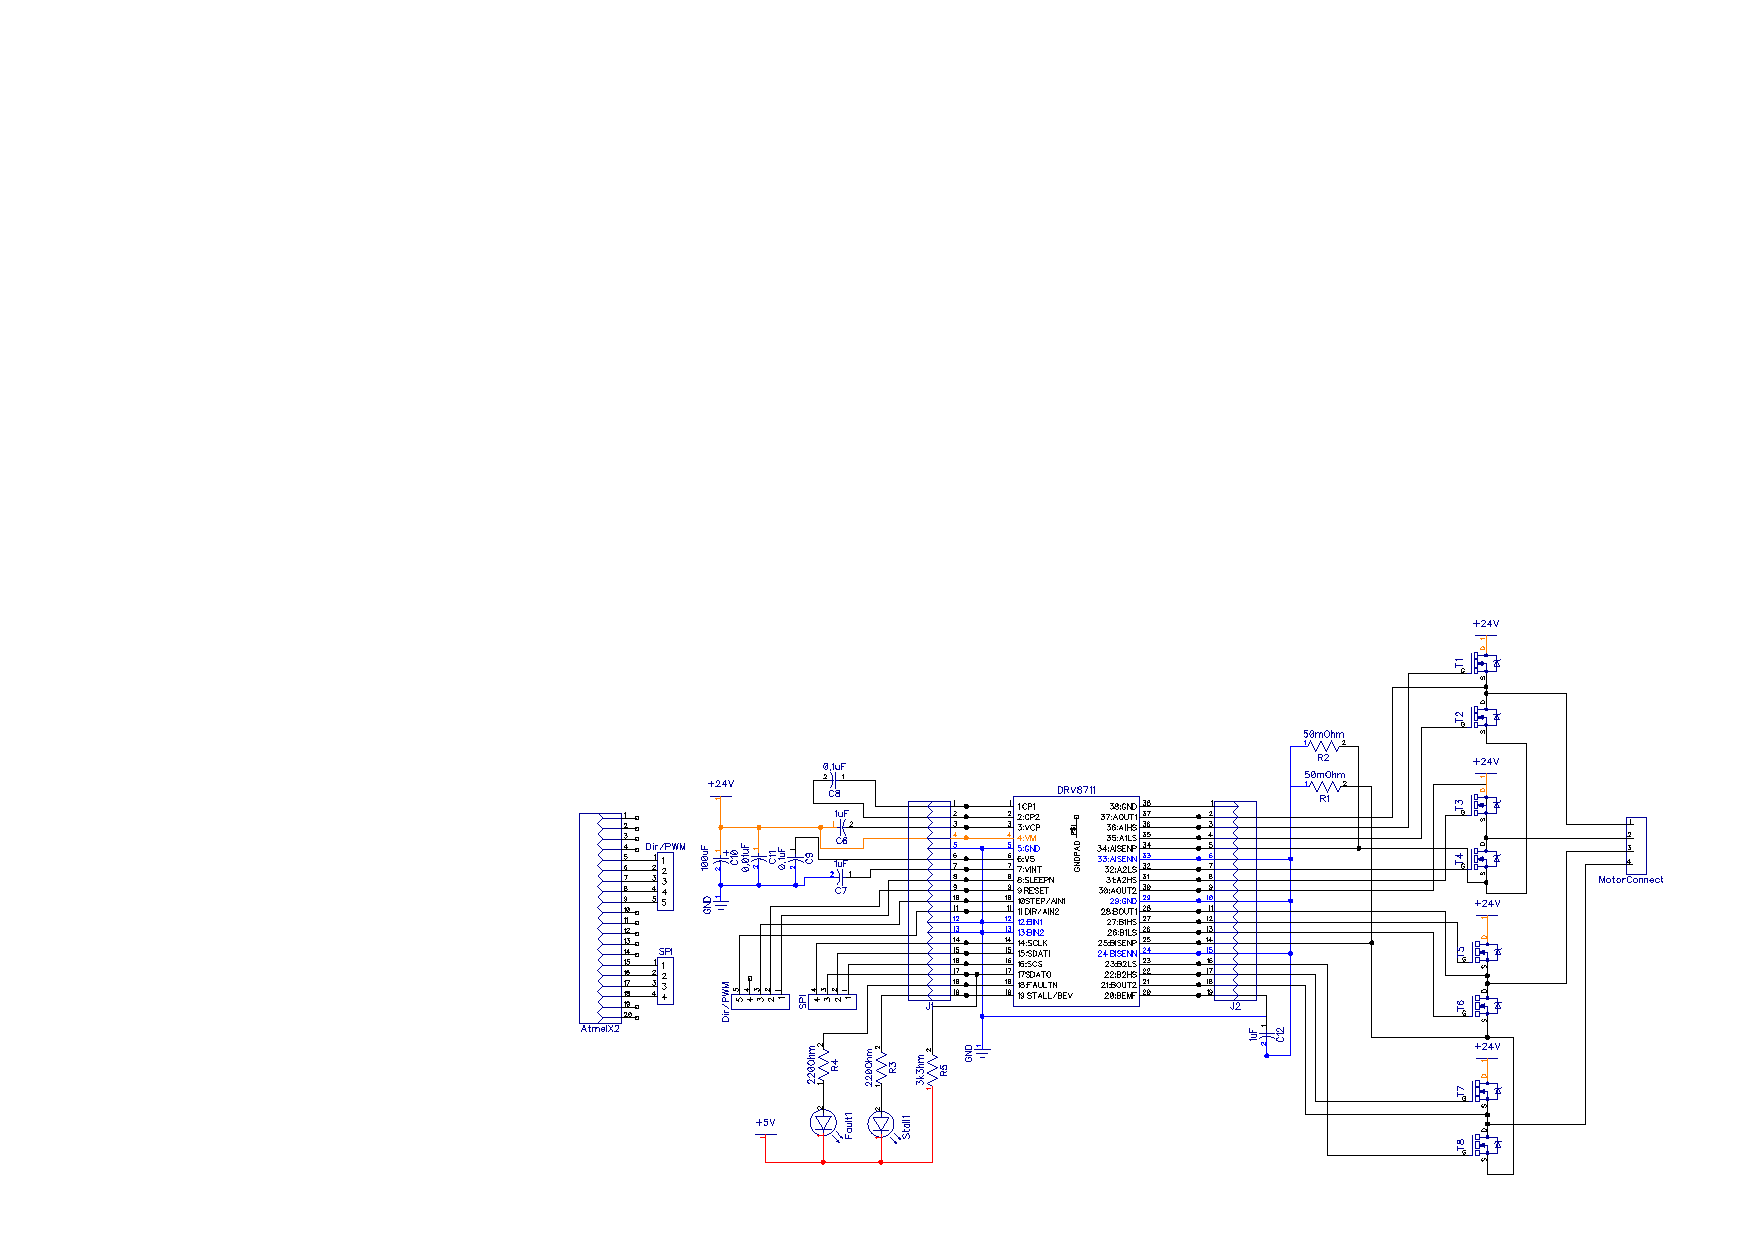
\includegraphics[width=1.3\textwidth]{pictures/scematic_drv8711.pdf}
   \caption[DRV8711 layout]{DRV8711 layout\\
	Source: Group 4  
  }
   \label{fig:DRV8711 layout}
\end{figure}
\end{landscape}

\subsection{Calculation}\label{sec:calculation_drv8711}

\subsubsection{Power Consumption of Sense Resistors}
The power dissipated by the sense resistor equals to \autoref{eq:power dissipation}.\\
$R_{ISENSE}=50*10^{-3}\Omega$\\
$I_{FS}=0,5371A$\\
$I_{FSpeak}=0,5371A*4=2,15A$
\begin{eqnarray}
P&=&I_{IFSpeak}^{2}*R_{ISENSE}\label{eq:power dissipation}\\
P&=&2,15^{2}*50*10^{-3}\Omega = 0,23W\label{eq:power dissipation result}
\end{eqnarray}
The sense resistor has a maximum $P_{dead}$ of $3W$ \footnote{see data sheet 3W\_0R050}. That means with the result of \autoref{eq:power dissipation result}, the sense resistor will never reach the $P_{dead}$.
\subsubsection{Drive Current}

From the data sheet \footnote{see data sheet DRV8711 page 13}, the following equation is used to calculate the drive current.
\begin{eqnarray}
I_{FS}&=&\frac{2,75V*TORQUE}{256*ISGAIN*R_{ISENSE}}\label{IFS formel}
\end{eqnarray}

With the following values \footnote{see at the register settings (\autoref{fig:DRV8711 registers}) and \autoref{tab:list of materials}} and the \autoref{IFS formel} the $I_{FS}$ is calculated. The result can bee seen at \autoref{eq:IFS ergebnis}.\\
$TORQUE=40$\\
$ISGAIN=100$\\
$R_{ISENSE}=50*10^{-3}\Omega$
\begin{eqnarray}
I_{FS}&=&\frac{2,75V*100}{256*40*50*10^{-3}\Omega}=0,5371A\label{eq:IFS ergebnis}
\end{eqnarray}

\subsubsection{Maximum allowed Drive Current}
It is necessary to calculate the maximum current for the \acs{MOSFET}'s, because we don't have a heat sink.
The following values are from the data sheet \footnote{see at IRF520 data sheet page 2}\\
$T_{j}=25^{\circ}C \, to \, 150^{\circ}C$\\
$T_{a}=25^{\circ}C$\\
$R_{DS(on)}=0,27\Omega$\\
$R_{thJA}=80^{\circ}K/W$\\
With the following equations, the maximum allowed current $I_{max}$ is calculated.
\begin{eqnarray}
T_{j}-T_{a}&=&R_{thJA}*P_{d}\\
P_{d}&=&U_{DS(on)}*I_{DS(on)}=I_{DS(on)}^{2}*R_{DS(on)}\\
T_{j}-T_{a}&=&I_{DS(on)}^{2}*R_{DS(on)}*R_{thJA}       \\
\rightarrow I_{max}&=&\sqrt{\frac{T_{j}-T_{a}}{R_{DS(on)}*R_{thJA}}}\\
 I_{max}&=&\sqrt{\frac{150^{\circ}C-25^{\circ}C}{0,27 \Omega * 80^{\circ}K/W}}=2,4A\label{eq:ergebnis_strom}
\end{eqnarray}
As we can see, the result from the \autoref{eq:ergebnis_strom} is lower than the maximum drive current (\autoref{eq:IFS ergebnis}). We chose a fuse (Fuse) with a value of $1,5A$ release current to protect the circuit.

\subsection{Measurements}
First the charge pump was measured and checked if there are $33V$ (\autoref{fig:DRV8711_charge_pump}) and also the \acs{VCP} should be $33V$ constantly. The measurement was done during the motor was driving. In \autoref{fig:DRV8711_charge_pump} the yellow probe shows the charge pump and the red probe shows \acs{VCP}.

\begin{figure}[H]
  \centering
   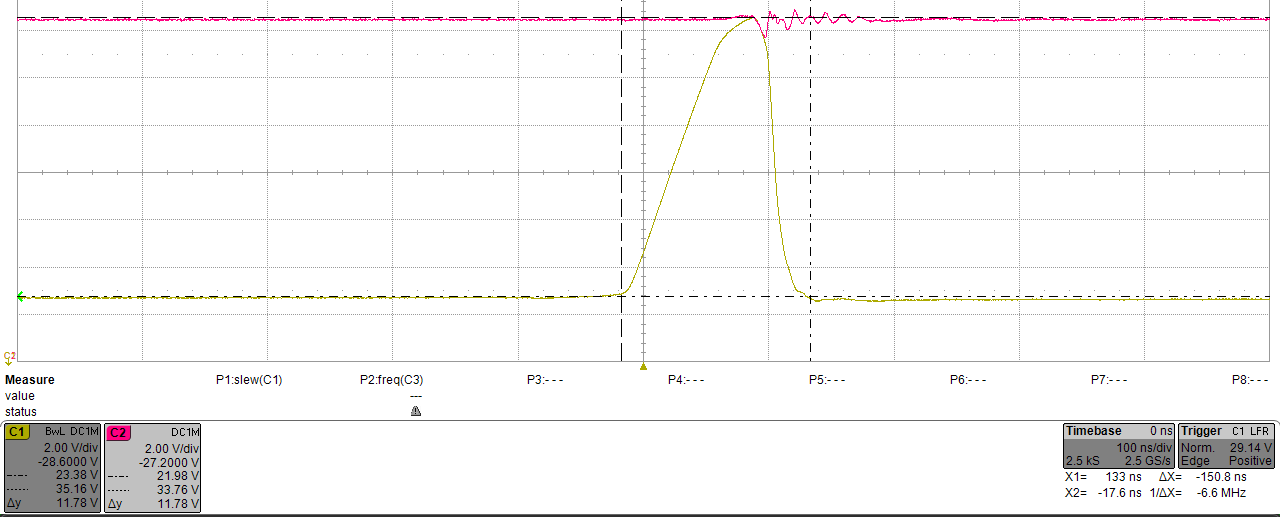
\includegraphics[width=1\textwidth]{pictures/measurements/DRV8711_charge_pump}
   \caption[Charge pump and \acs{VCP}]{charge pump and \acs{VCP}\\
	Source: Group 4  
  }
   \label{fig:DRV8711_charge_pump}
\end{figure}

AS can be seen, the values are like we expected it.

Secondly the \acs{SPI} configuration is send with an \acs{SPI} simulator. \autoref{fig:SPI_send_config_measurement} shows the telegram for the configuration and \autoref{fig:SPI_send_status_measurement} shows the telegram to get the status. Channel 1 (yellow probe) shows the \acs{SPI} data output, Channel 2 (red probe) shows the \acs{SPI} clock, Channel 3 (blue probe) shows the \acs{SPI} data input from the DRV8711 and Channel 4 (green probe) shows the \acs{SPI} chip select. Don't bee confused, about the chip select, its an active high output.

\begin{figure}[H]
  \centering
   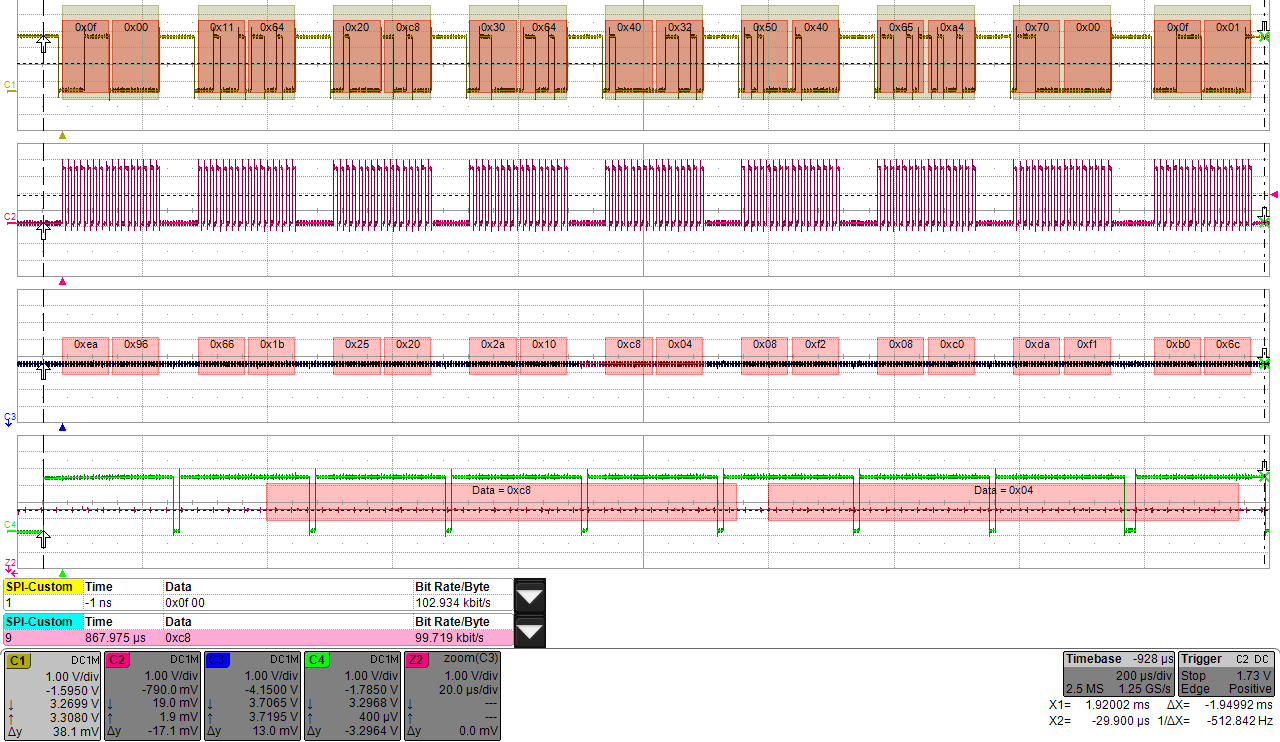
\includegraphics[width=1\textwidth]{pictures/measurements/SPI_send_config_measurement}
   \caption[\acs{SPI} send configuration]{\acs{SPI} send configuration\\
	Source: Group 4  
  }
   \label{fig:SPI_send_config_measurement}
\end{figure}

\begin{figure}[H]
  \centering
   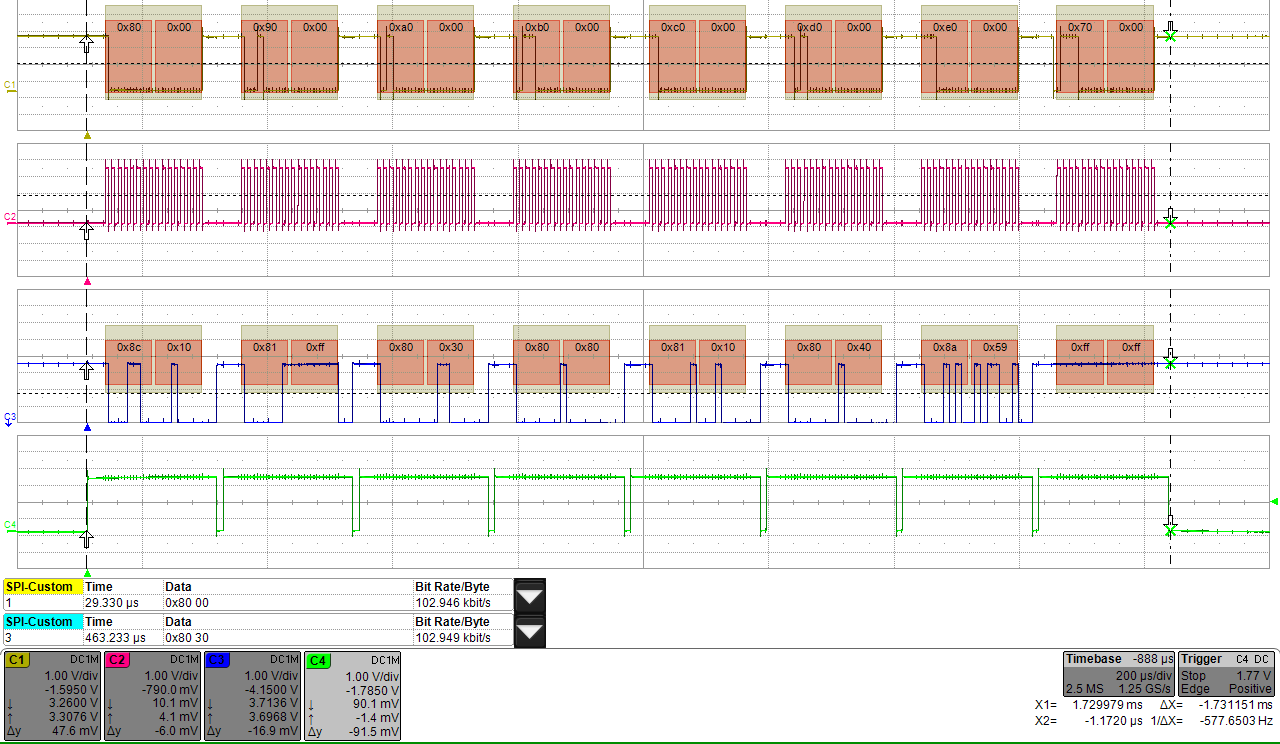
\includegraphics[width=1\textwidth]{pictures/measurements/SPI_send_status_measurement}
   \caption[\acs{SPI} get status]{\acs{SPI} get status\\
	Source: Group 4  
  }
   \label{fig:SPI_send_status_measurement}
\end{figure}

As can bee seen, the \acs{SPI} works good.

Thirdly the H-bridges are measured and the motor current (\autoref{fig:DRV8711_current_mosfets.png}). The yellow probe is the A1HS and the red one the B1HS. The blue probe is the frequency the \acs{uC} is sending.

\begin{figure}[H]
  \centering
   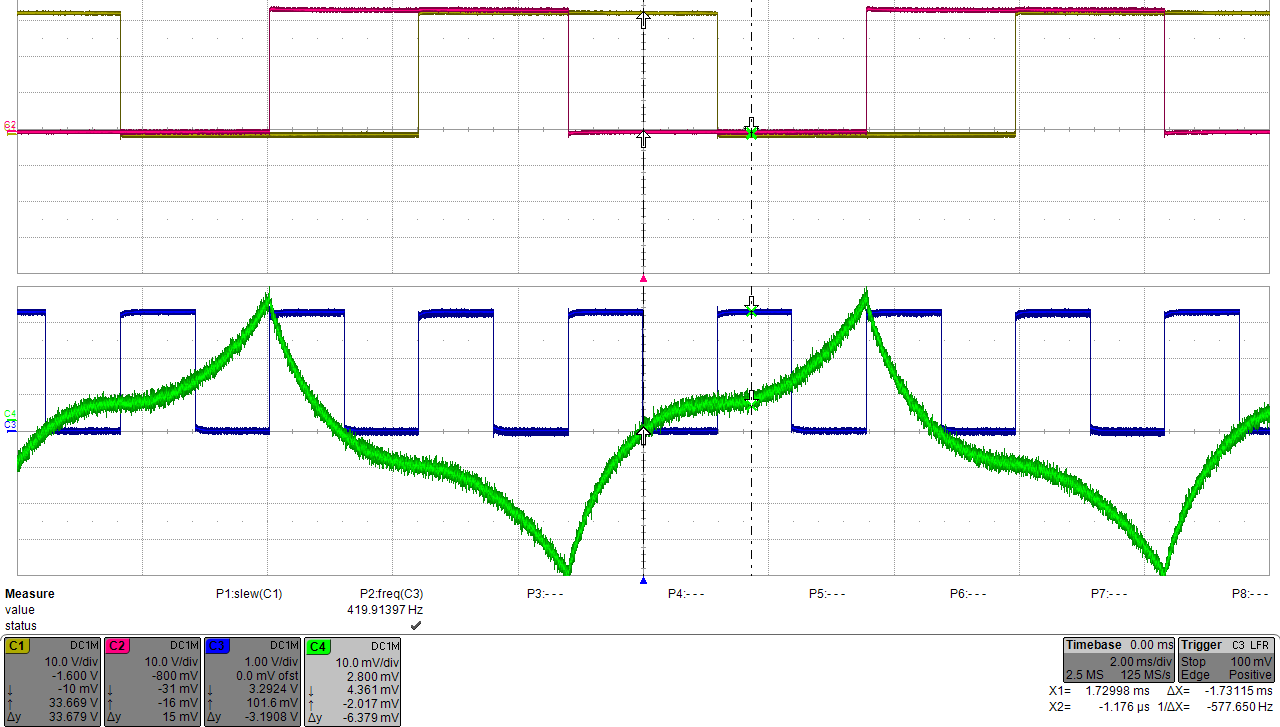
\includegraphics[width=1\textwidth]{pictures/measurements/DRV8711_current_mosfets.png}
   \caption[DRV8711 H-Bridges Voltage and motor current]{DRV8711 H-Bridges and motor current\\
	Source: Group 4  
  }
   \label{fig:DRV8711_current_mosfets.png}
\end{figure}
As can bee seen, the H-bridges are switching perfectly, but the motor current is not like it should be. We tried hard to get a nice sinus, but we did not find any other good configuration. Therefore we chose this configuration, because it drives smoothly.

\section{Emergency Stop and limit Switch Circuit}
\subsection{Description}
The emergency stop is a potential free contact. The available parts has a safety relay, a left over contact is used to switch the relay (Relais, Schrack, A1, A2). The \acs{uC} uses a a contact (5, 4) of the relay, to detect if the emergency circuit is released. A capacitor (C17) is used to debounce the signal.\\
The limit switch is used to detect the home position. It is implemented as normally closed contact, to detect wire breaks. It is also a A capacitor (C16) used to debounce the signal.\\
There are 4 connectors (AtmelX3, LimitSwitch, EmergencyStop24V, EmergencyStoptouC) to linkt the wires to the \acs{uC}, limit switch and the Schrack relay.

\subsection{Measurement}

 the signal was analysed without (\autoref{fig:limitSwitch_without_capacitor_1}) and with (\autoref{fig:limitSwitch_with_capacitor_1}) capacitor. To test if it works correctly in the field, the limit switch and the emergency circuit are called in an interrupt for each switch in the \acs{uC}. The interrupt is called correctly, the value of the capacitor to debounce is correct.

\begin{figure}[H]
  \centering
   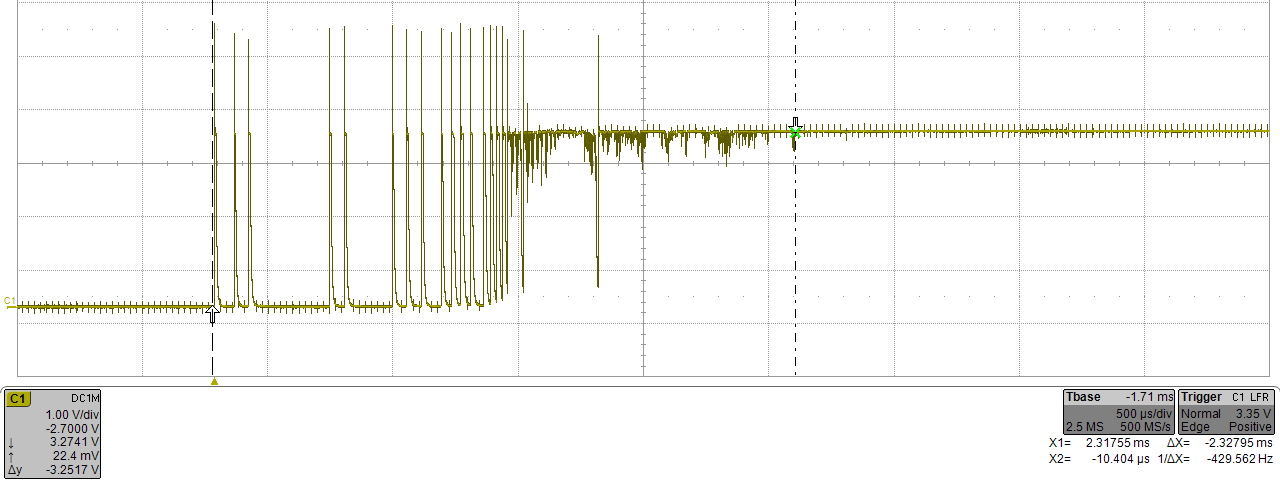
\includegraphics[width=1\textwidth]{pictures/measurements/limitSwitch_without_capacitor_1}
   \caption[Switch without capacitor]{Switch without capacitor\\
	Source: Group 4  
  }
   \label{fig:limitSwitch_without_capacitor_1}
\end{figure}

\begin{figure}[H]
  \centering
   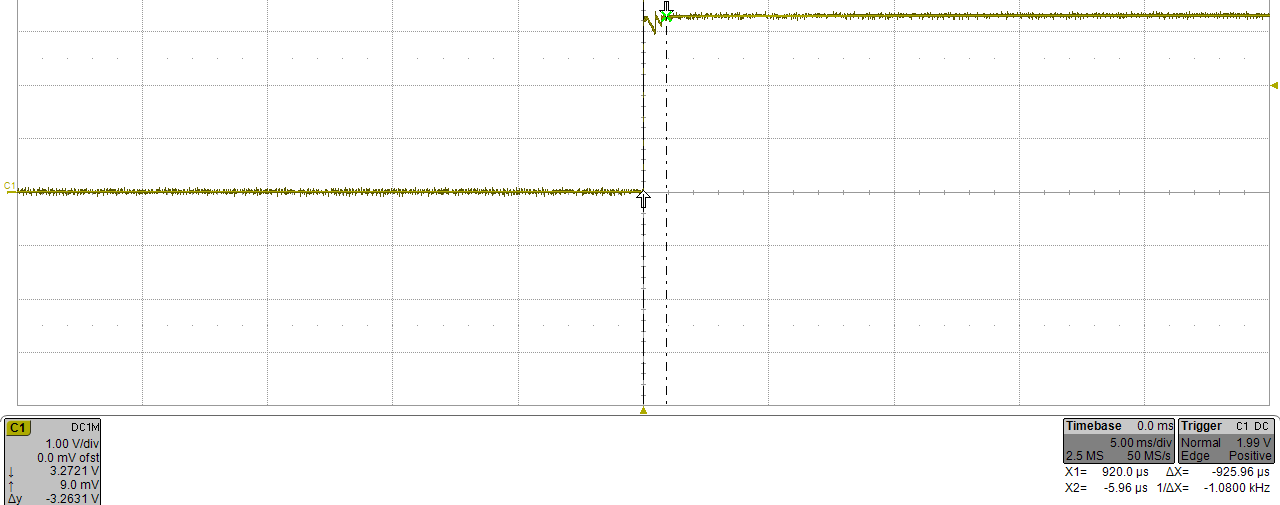
\includegraphics[width=1\textwidth]{pictures/measurements/limitSwitch_with_capacitor_1}
   \caption[Switch with capacitor]{Switch with capacitor\\
	Source: Group 4  
  }
   \label{fig:limitSwitch_with_capacitor_1}
\end{figure}



\subsection{Schematic}
In \autoref{fig:emergency and limit switch} is the schematic shown from the emergency relay and the limit switch. There was no need to do a \acs{PCB} layout, because we soldered it just together.
\begin{figure}[H]
  \centering
   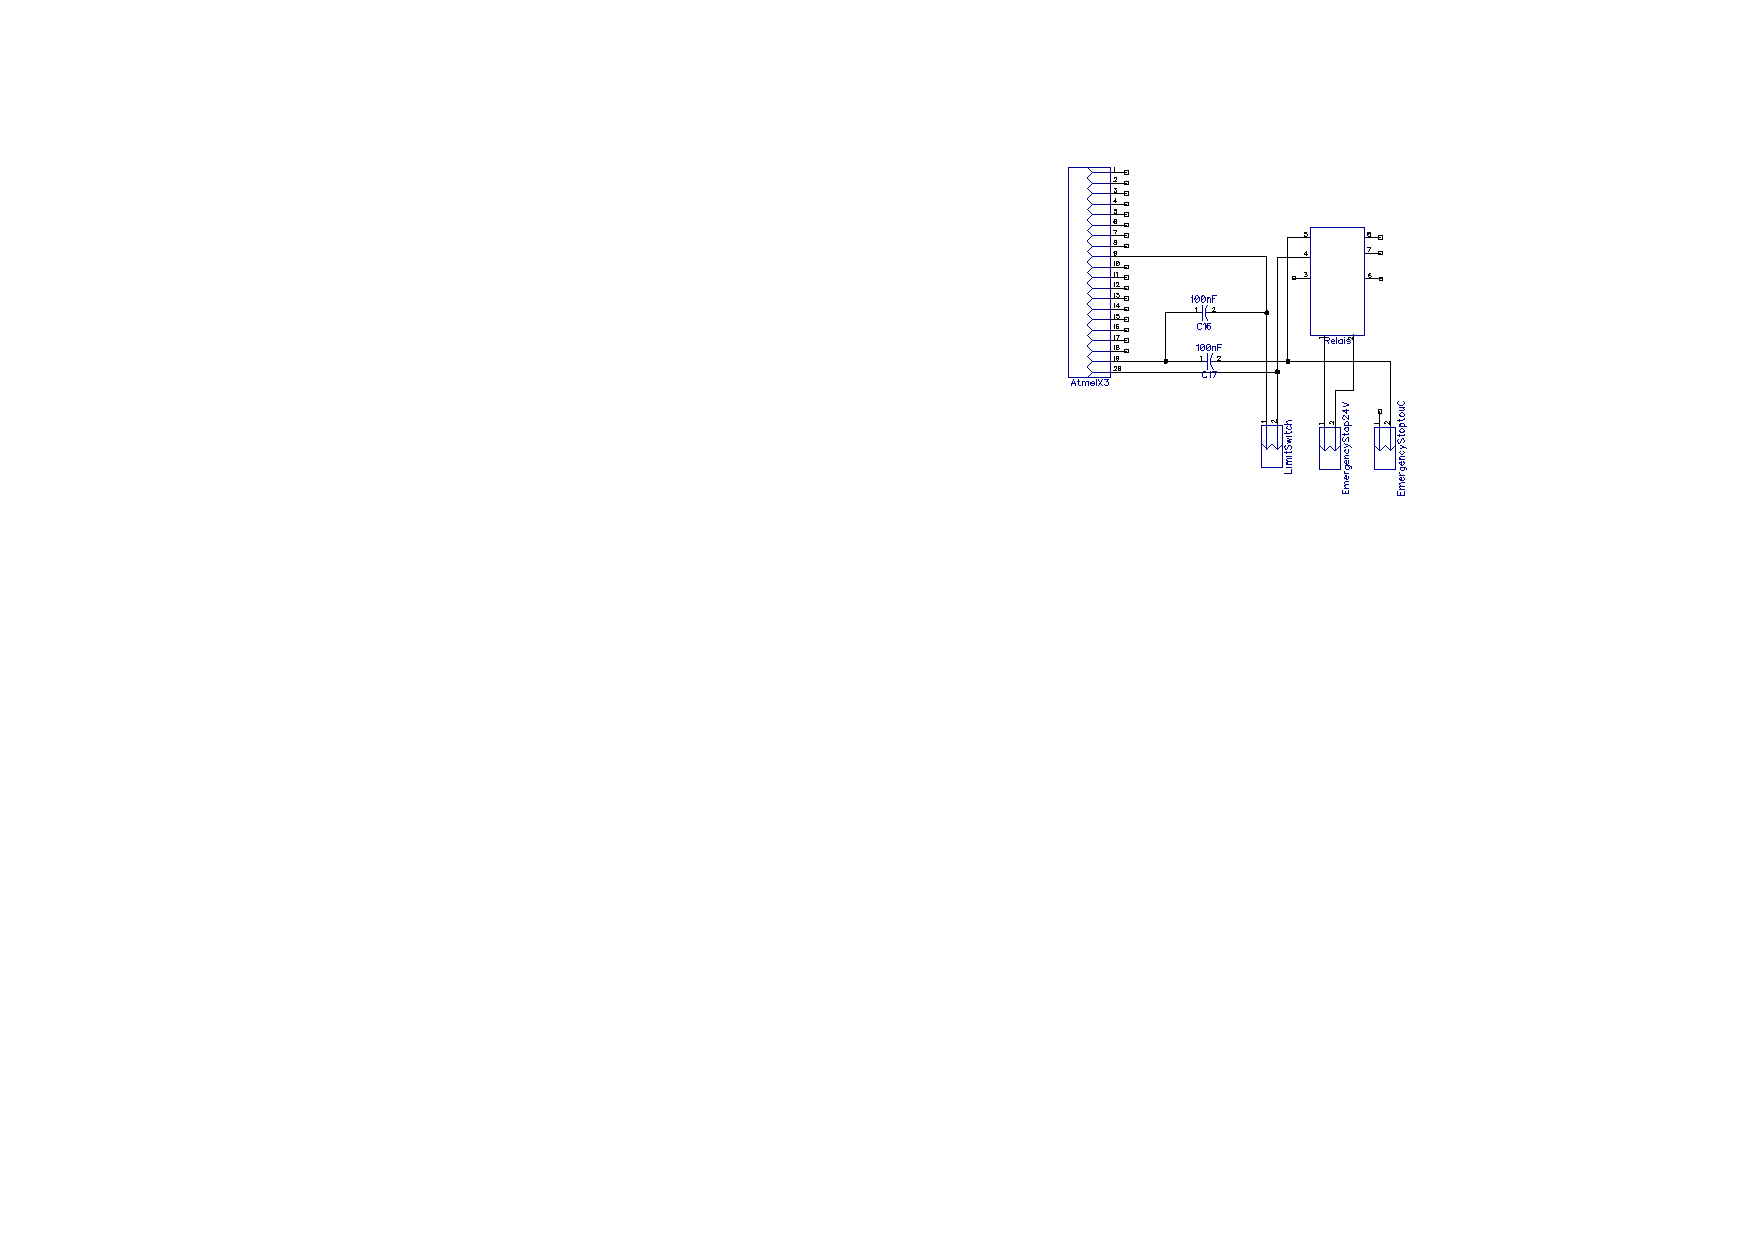
\includegraphics[width=1\textwidth]{pictures/scematic_switch_emergency.pdf}
   \caption[Emergency and limit switch schematic]{Emergency and limit switch schematic\\
	Source: Group 4  
  }
   \label{fig:emergency and limit switch}
\end{figure}


\section{Bill of materials}
In \autoref{tab:list of materials} the bill of materials can be found for parts that are used to build the amplifier.

\begin{table}[H]
\centering
\begin{tabular}{|p{5.5cm}|p{2cm}|p{5.3cm}|p{2cm}|}
\hline
\textbf{Definition in circuit            }               				     & \textbf{Value}  			& \textbf{Name}          & \textbf{Quantity} \\ \hline
AtmelPWR                                         				&        				& PPTC022LFBN-RC  & 1        \\ \hline
AtmelX1, AtmelX2, AtmelX3                        		&        				& PPTC102LFBN-RC  & 3        \\ \hline
C1, C2, C3, C4, C5, C6, C7, C12, C15              & $1 \mu F$   			& CAP\_0603  (ceramic)     & 9        \\ \hline
C8, C9                                           					& $0,1 \mu F$  			& CAP\_0603  (ceramic)     & 2        \\ \hline
C10                                             						& $100 \mu F$ 			& EEE--CASE-E (electrolyte)    & 1        \\ \hline
C11                                            						& $0,01 \mu F$ 			& CAP\_0603  (ceramic)      & 1        \\ \hline
C13, C14                                         					& $10 \mu F$   			& CAP\_1206   (tantalum)     & 2        \\ \hline
C16, C17                                         					& $100 \mu F$  			& CAP100      (ceramic)    & 2        \\ \hline
DMSConnector                                     				&        				& PINHD-1X4       & 1        \\ \hline
DRV8711                                          					&       			 	& DRV8711         & 1        \\ \hline
EmergencyStop24V, EmergencyStoptouC, LimitSwitch 				&        & HDR-1x2         & 3        \\ \hline 
Fault1, Stall1                                   					&        				& LED             & 2        \\ \hline
Fuse1                                            					&        				& Fuse            & 1        \\ \hline
INA128UA1                                        				&        				& INA128UA        & 1        \\ \hline
J1, J2                                           						&        				& HDR-1x19        & 2        \\ \hline
linearVoltageRegulator                           			&        				& LM1086IS-5.0    & 1        \\ \hline
MotorConnector                                   				&        				& MSTB 2-5-5,08x4 & 1        \\ \hline
Power24V                                         				&        				& MSTB 2-5-5,08x2 & 1        \\ \hline
R1, R2                                           					& $50m \Omega$ 		& PowerResistor   & 2        \\ \hline
R3, R4                                           					& $220\Omega$ 		& RES\_0603       & 2        \\ \hline
R5                                               						& $3,3k\Omega$ 		& RES\_0603       & 1        \\ \hline
R6, U1                                           					& $500\Omega$ 		& POT             & 2        \\ \hline
Relais                                           						&        				& Schrack         & 1        \\ \hline
RS232Shfiter                                     				&        				& MAX232          & 1        \\ \hline
T1, T2, T3, T4, T5, T6, T7, T8                   		&        				& IRF520          & 8       \\ \hline
\end{tabular}
\caption{List of materials}
\label{tab:list of materials}
\end{table}

\section{\acs{PCB} layout}
In \autoref{fig:PCB layout} the designed layout is shown. We tried to separate the power (motor driver) and digital (amplifier, \acs{RS232} shifter) circuits to reduce noises. We also used star point grounding for the analogue components, such as the amplifier. Additional we tried to separate the analogue and digital ground. We decided to do the soldering for the most parts with the pick and place machine. Only the \acs{IC}'s and the connectors has to be soldered by hand.
  \begin{figure} [H]
        \centering
        \begin{subfigure}[b]{0.65\textwidth}
                \centering
                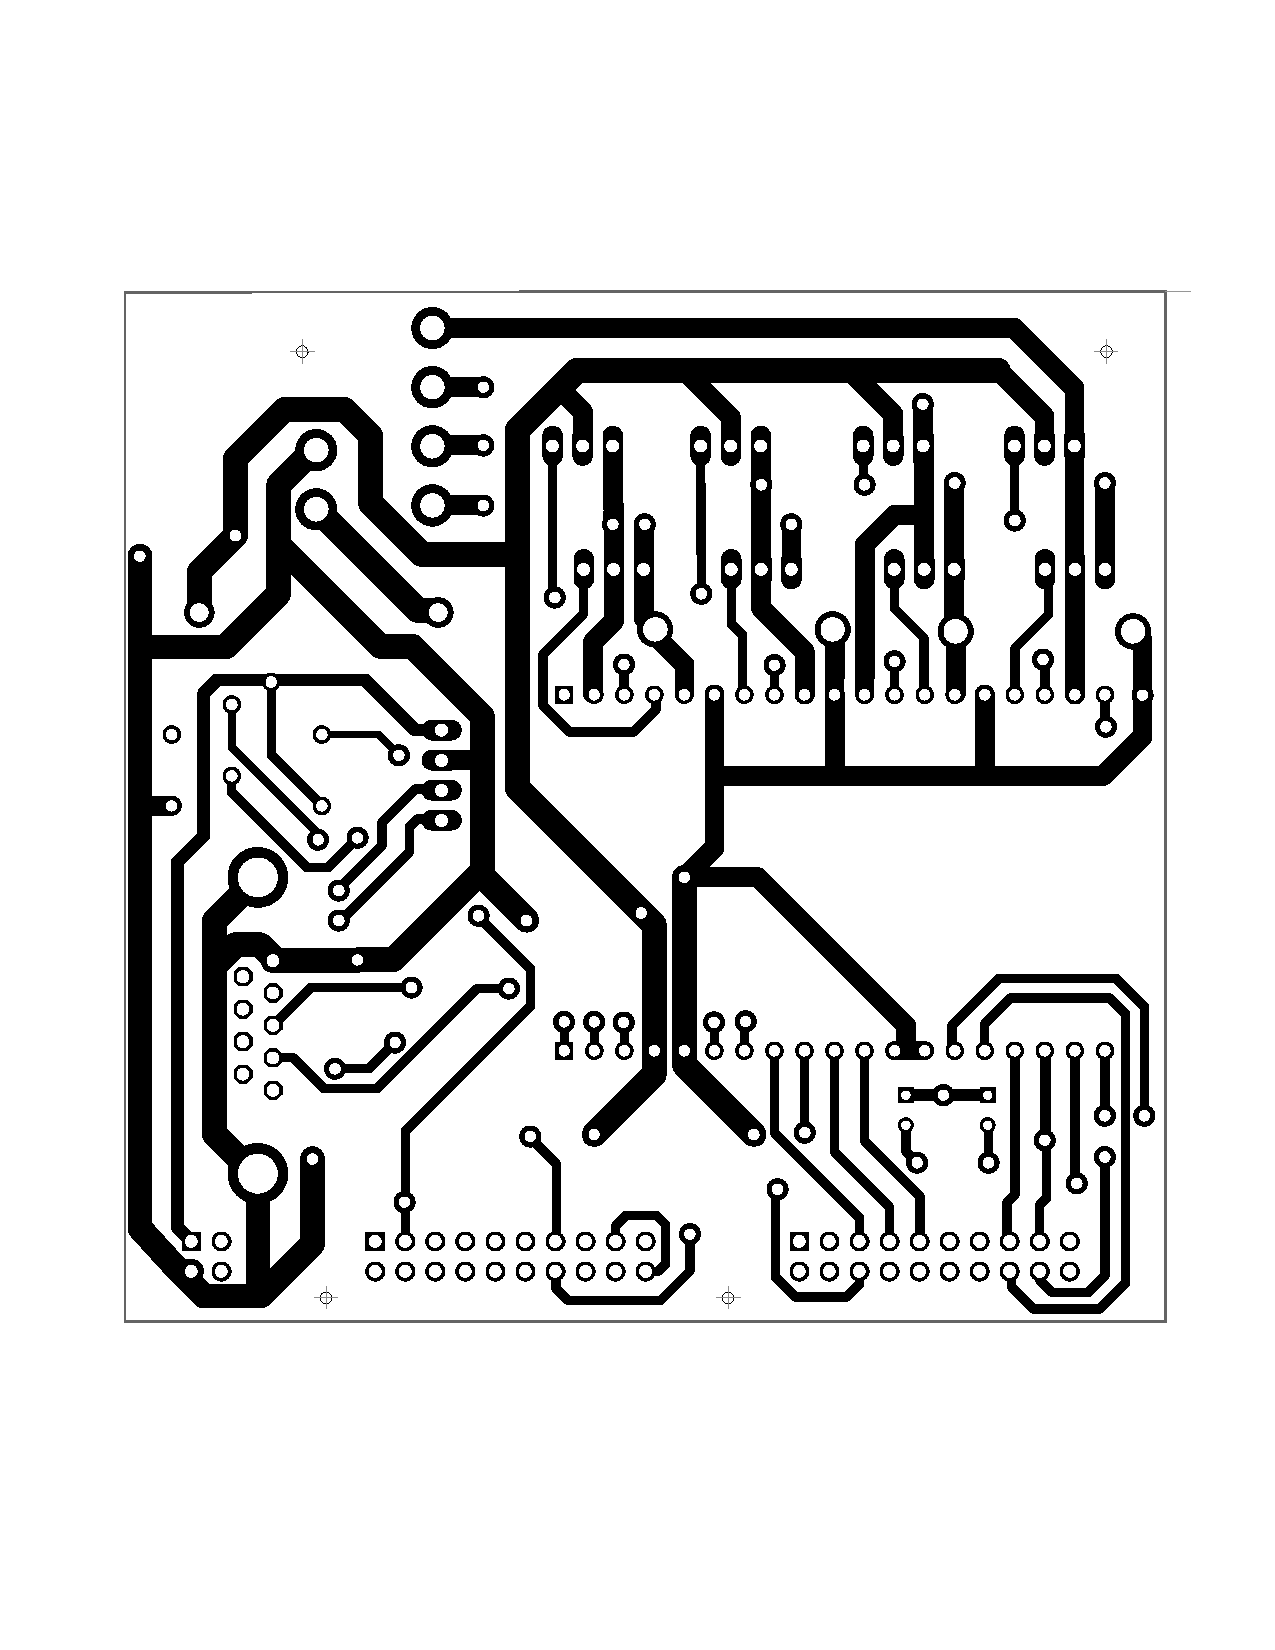
\includegraphics[width=0.9\textwidth]{pictures/PCB_BOTTOM_v_2_0.pdf}
                \caption{Bottom}\label{fig:pcb_bottom}
        \end{subfigure}%
        ~ % An dieser Stelle kann ein zusätzlicher Zwischenraum eingebunden werden: ~, \quad, \qquad, \hfill usw.
          % Eine leere Zeile erzwingt, dass die zweite Grafik darunter erscheint.
          
        \begin{subfigure}[b]{0.65\textwidth}
                \centering
                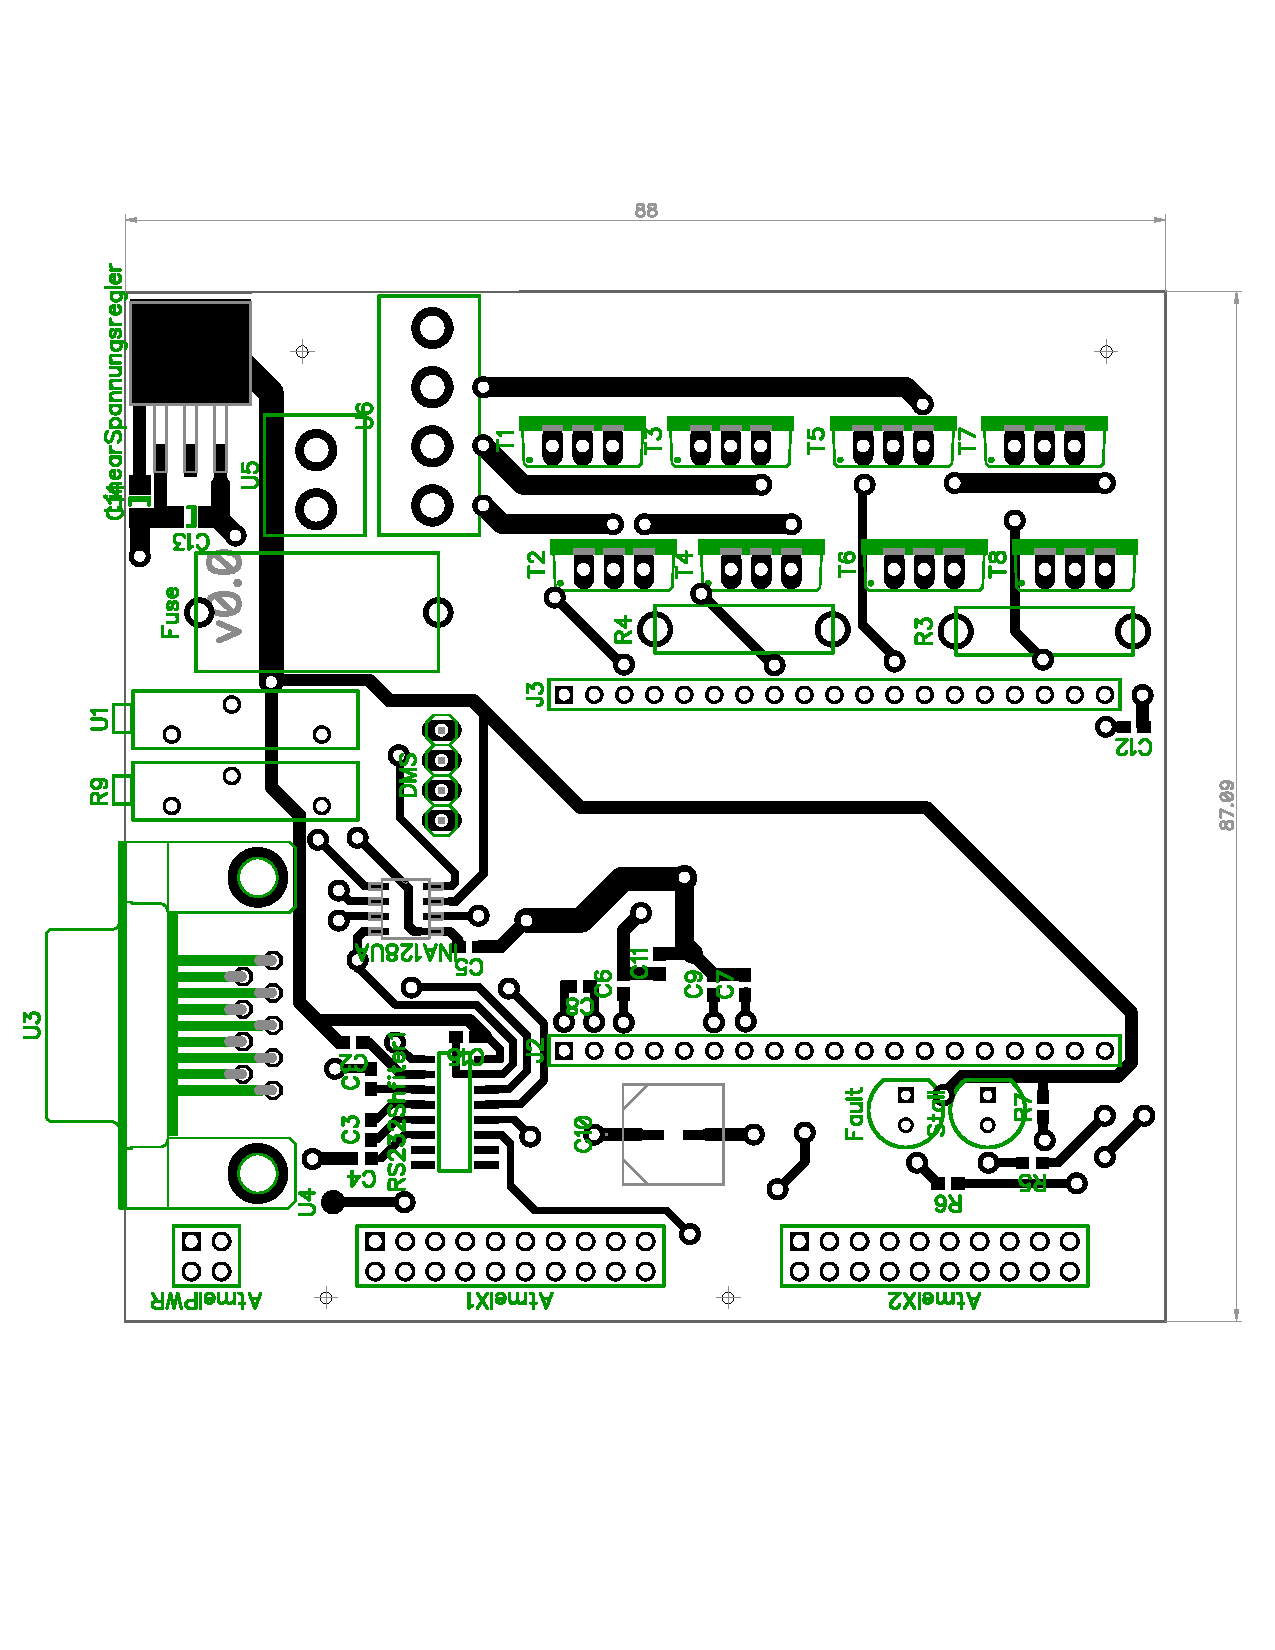
\includegraphics[width=1\textwidth]{pictures/PCB_TOP_v_2_0.pdf}
                \caption{Top}\label{fig:pcb_top}
        \end{subfigure}
        \caption[Bottom and top \acs{PCB} layout]{bottom and top \acs{PCB} layout\\
		source: group 4        
        }\label{fig:PCB layout}
  \end{figure}

In \autoref{fig:PCB layout} the rendered \acs{PCB} layout is show.
  
\begin{figure}[H]
  \centering
   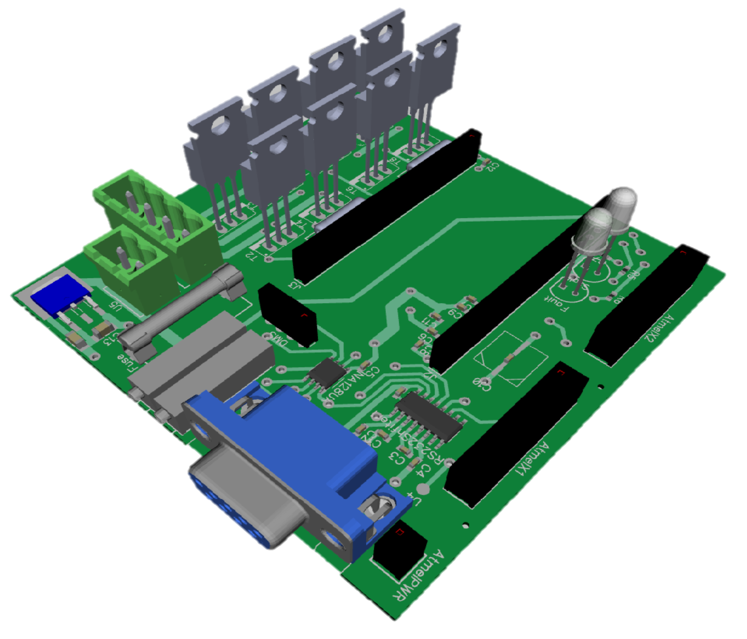
\includegraphics[width=1\textwidth]{pictures/PCB_Rendered}
   \caption[Rendered PCB Layout]{Rendered PCB Layout\\
	Source: Group 4  
  }
   \label{fig:PCB_Rendered}
\end{figure}  

\chapter{\acs{PLC}-Program}

The program which controls the whole system runs on regular PC. Programming is mainly made using Visual Studio and on it twinCAT3 extension. The program controls the X, Y and Z axes and provides \acs{HMI} for that. The main focus of the program is to provide cycles for picking and dropping the object. The other parts of the program manage information, for example managing data provided by \acs{uC} and showing the force when picking the object.  It also have an error handling functions such as \enquote{emergency button pressed} or \enquote{too much force applied}. 
\section{Main Program}
Main program contains all the functions to move axes and subprograms to do error handling and force measuring. The homing function is executed after the button is pressed. When homing the first time the X and Y axes will first reference, using the limit switches. After that moving from the reference position (X: $0,0$, Y: $0,0$) to the home position. After pick or drop cycle the axes move right to the home position.\\
The picking cycle can be executed from the home position by pushing the button. As an example of programming, picking disc from \acs{Repository} has three steps. The first step is to move above the disc.  The second is snapping the disc. And the third is sliding the disc away from the \acs{Repository} and moving to the home position. Every executed function that is set true, must be set false afterwards as seen from the examples.\\

 \lstset{
   basicstyle=\scriptsize\ttfamily,
   keywordstyle=\bfseries\ttfamily\color{orange},
   stringstyle=\color{green}\ttfamily,
   commentstyle=\color{middlegray}\ttfamily,
   emph={square}, 
   emphstyle=\color{blue}\texttt,
   emph={[2]root,base},
   emphstyle={[2]\color{yac}\texttt},
   showstringspaces=false,
   flexiblecolumns=false,
   tabsize=2,
   numbers=left,
   numberstyle=\tiny,
   numberblanklines=false,
   stepnumber=1,
   numbersep=11pt,
   xleftmargin=15pt,
   breaklines=true
 }
 \lstinputlisting
    [caption={Homing axes}
       \label{lst:istate15-21},
       captionpos=t,language=pascal,firstnumber=44]
       {listings/homing.xml}
       
        \lstinputlisting
    [caption={Moving above the disc}
       \label{lst:moving above the disc},
       captionpos=t,language=pascal,firstnumber=43]
 {listings/movingAboveDisk.xml}
 
  \lstinputlisting
    [caption={Snapping the disc}
       \label{lst:snapping the disc},
       captionpos=t,language=pascal,firstnumber=42]
 {listings/snappingDisk.xml}

The values of different steps are stored in array when the program starts running. The steps are:
\begin{itemize}
\item postRepository: \acs{Repository} during picking or dropping. (X: $136,75$, Y: $0,2$)
\item pastPrepositioning: Before/after moving sideways in/out of the \acs{Repository}. (X: $136,75$, Y: $125,0$).
\item posHome: The home position. (X: $15,0$, Y: $400,0$).
\end{itemize}

If the system response from system takes too much time the program retry. In the code it can be seen, for example in line 33 of \autoref{lst:snapping the disc}. After failing the program tries again from line 31.

In \autoref{fig:drop_pickcylce} the loop of the main program is shown according to the \acs{UML} standards.

\begin{figure}[H]
  \centering
   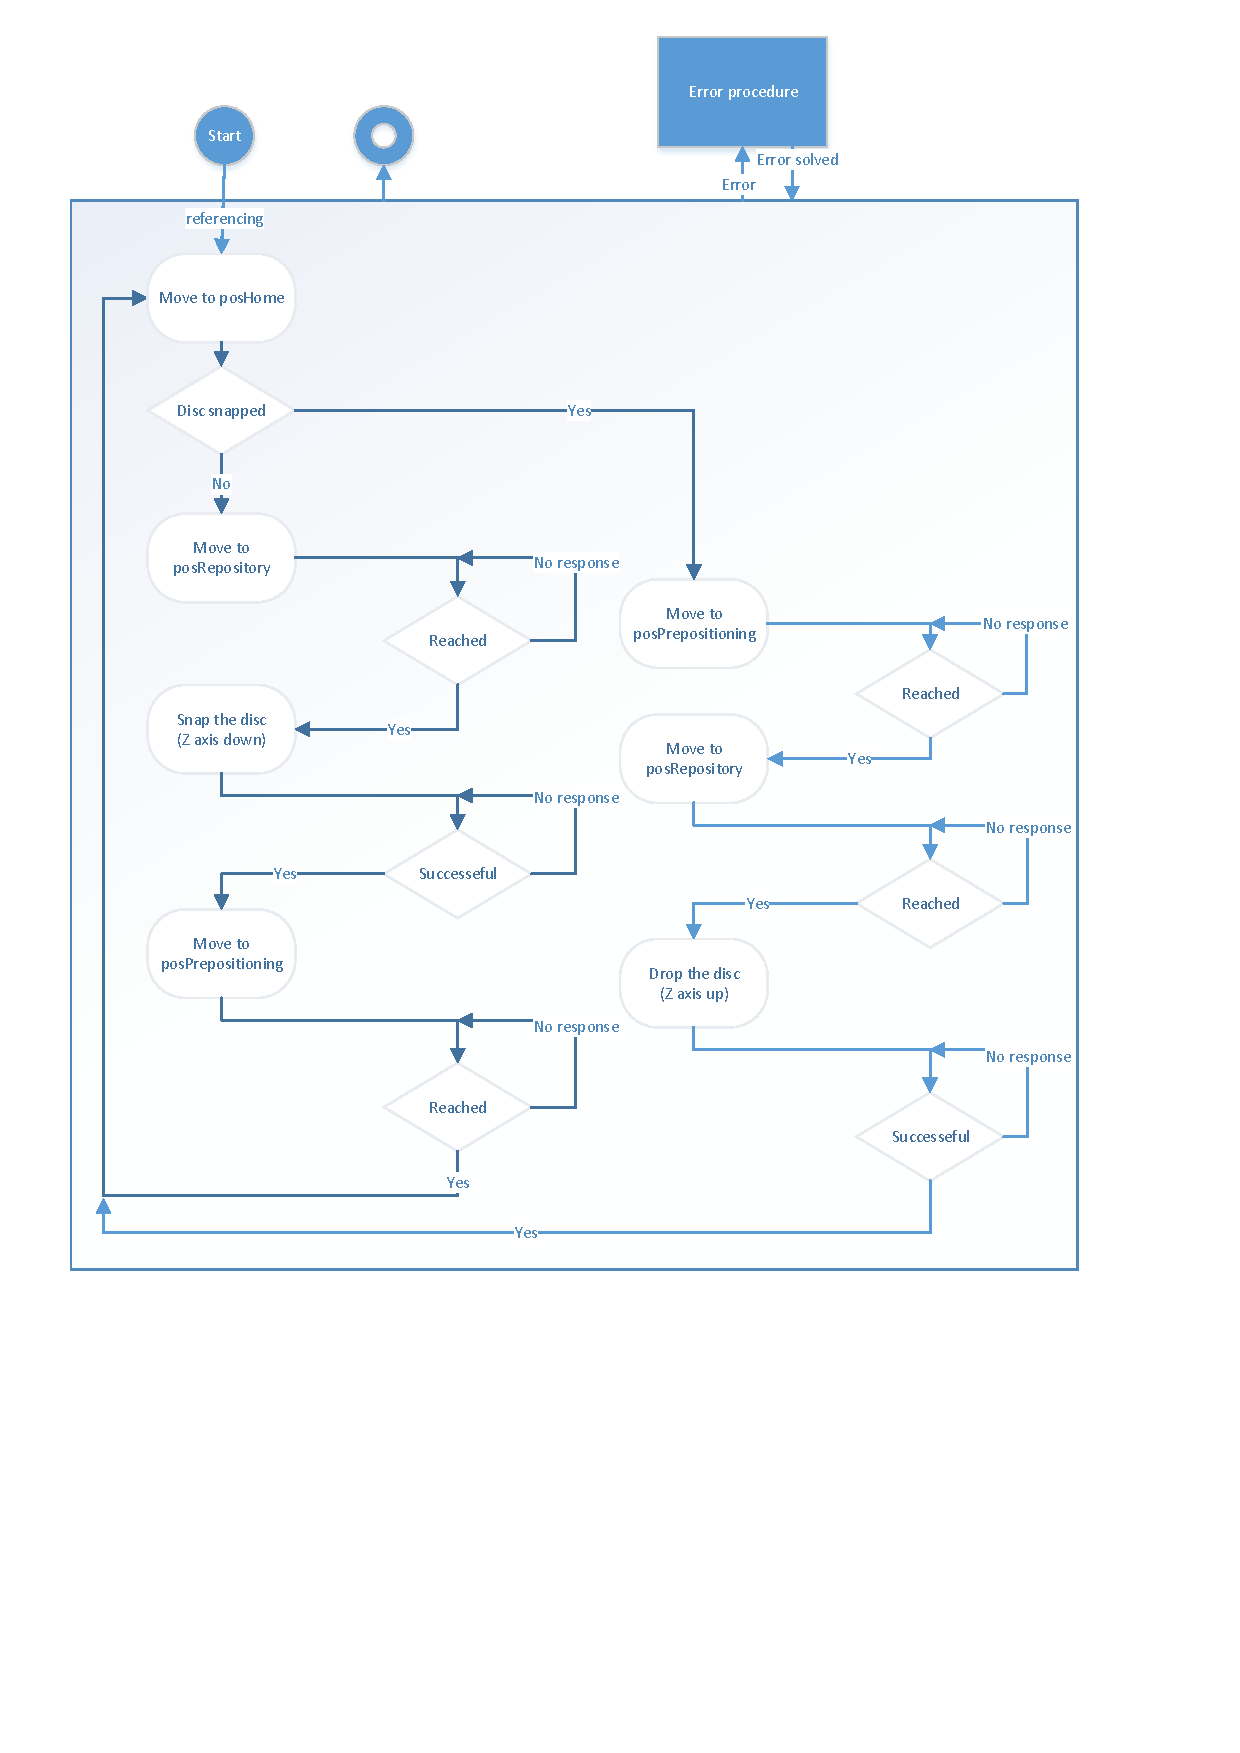
\includegraphics[width=0.9\textwidth]{pictures/VisioDropcycle.pdf}
   \caption[Flowchart of pick and drop cycle]{Flowchart of pick and drop cycle\\
	Source: Group 4}
   \label{fig:drop_pickcylce}
\end{figure} 

\section{Error Procedure}
The program has some error handling functions in addition of emergency stop. These are:
\begin{itemize}
\item No disc detected
\item Too much force on strain gauge. (the maximum and minimum forces are 10N)
\item No power from the motors of X, Y axes
\item Error signal from \acs{uC}
\item Emergency stop is pressed
\end{itemize}
If the system counters error during run, all of the movement stops. If the disc is on the snapper it must be manually removed. After solving other possible error/errors the reset button must be pressed to run the system again. The Z-axis referencing every time after error for the X and Y axes that's not necessary.

\section{\acs{HMI}}
The \acs{HMI} is made to be as simple as possible. There are however some extra features like continuously run, which is mainly meant for maintaining. The graphs shows the positions of axes in real time, in the graph and also the exact number is shown. Also there is graph and number that have the current status of force gauge. Force units are in $mN$. The minimum and maximum forces are saved. Status, report and debug messages are kept in a message board, at top right corner of the \acs{HMI}.

\begin{figure}[H]
  \centering
   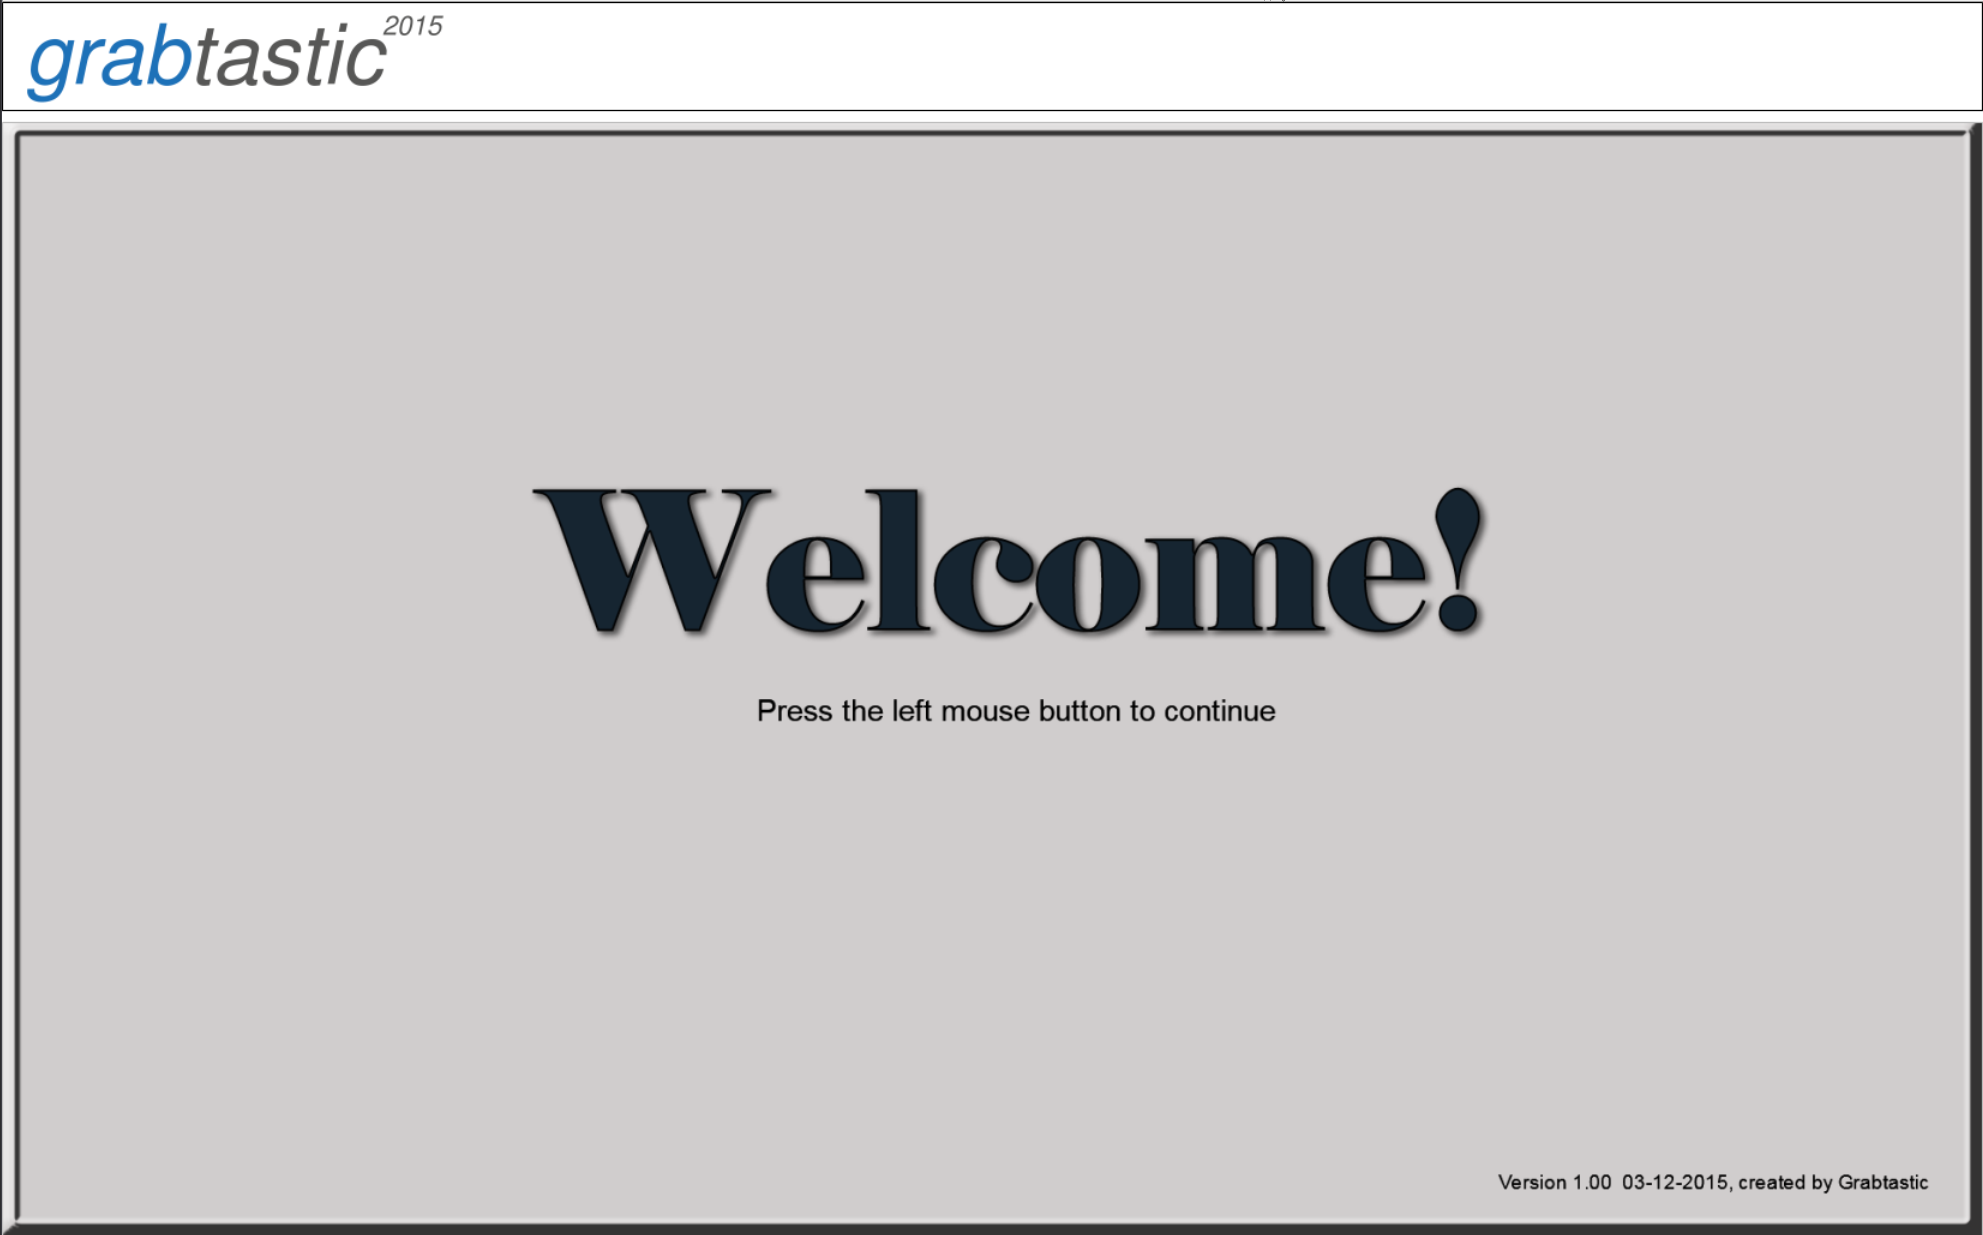
\includegraphics[width=0.7\textwidth]{pictures/Welcome1080}
   \caption[Welcome screen]{Welcome screen\\
	Source: Group 4}
   \label{fig:start view}
\end{figure} 

\begin{landscape}
\begin{figure}[H]
  \centering
   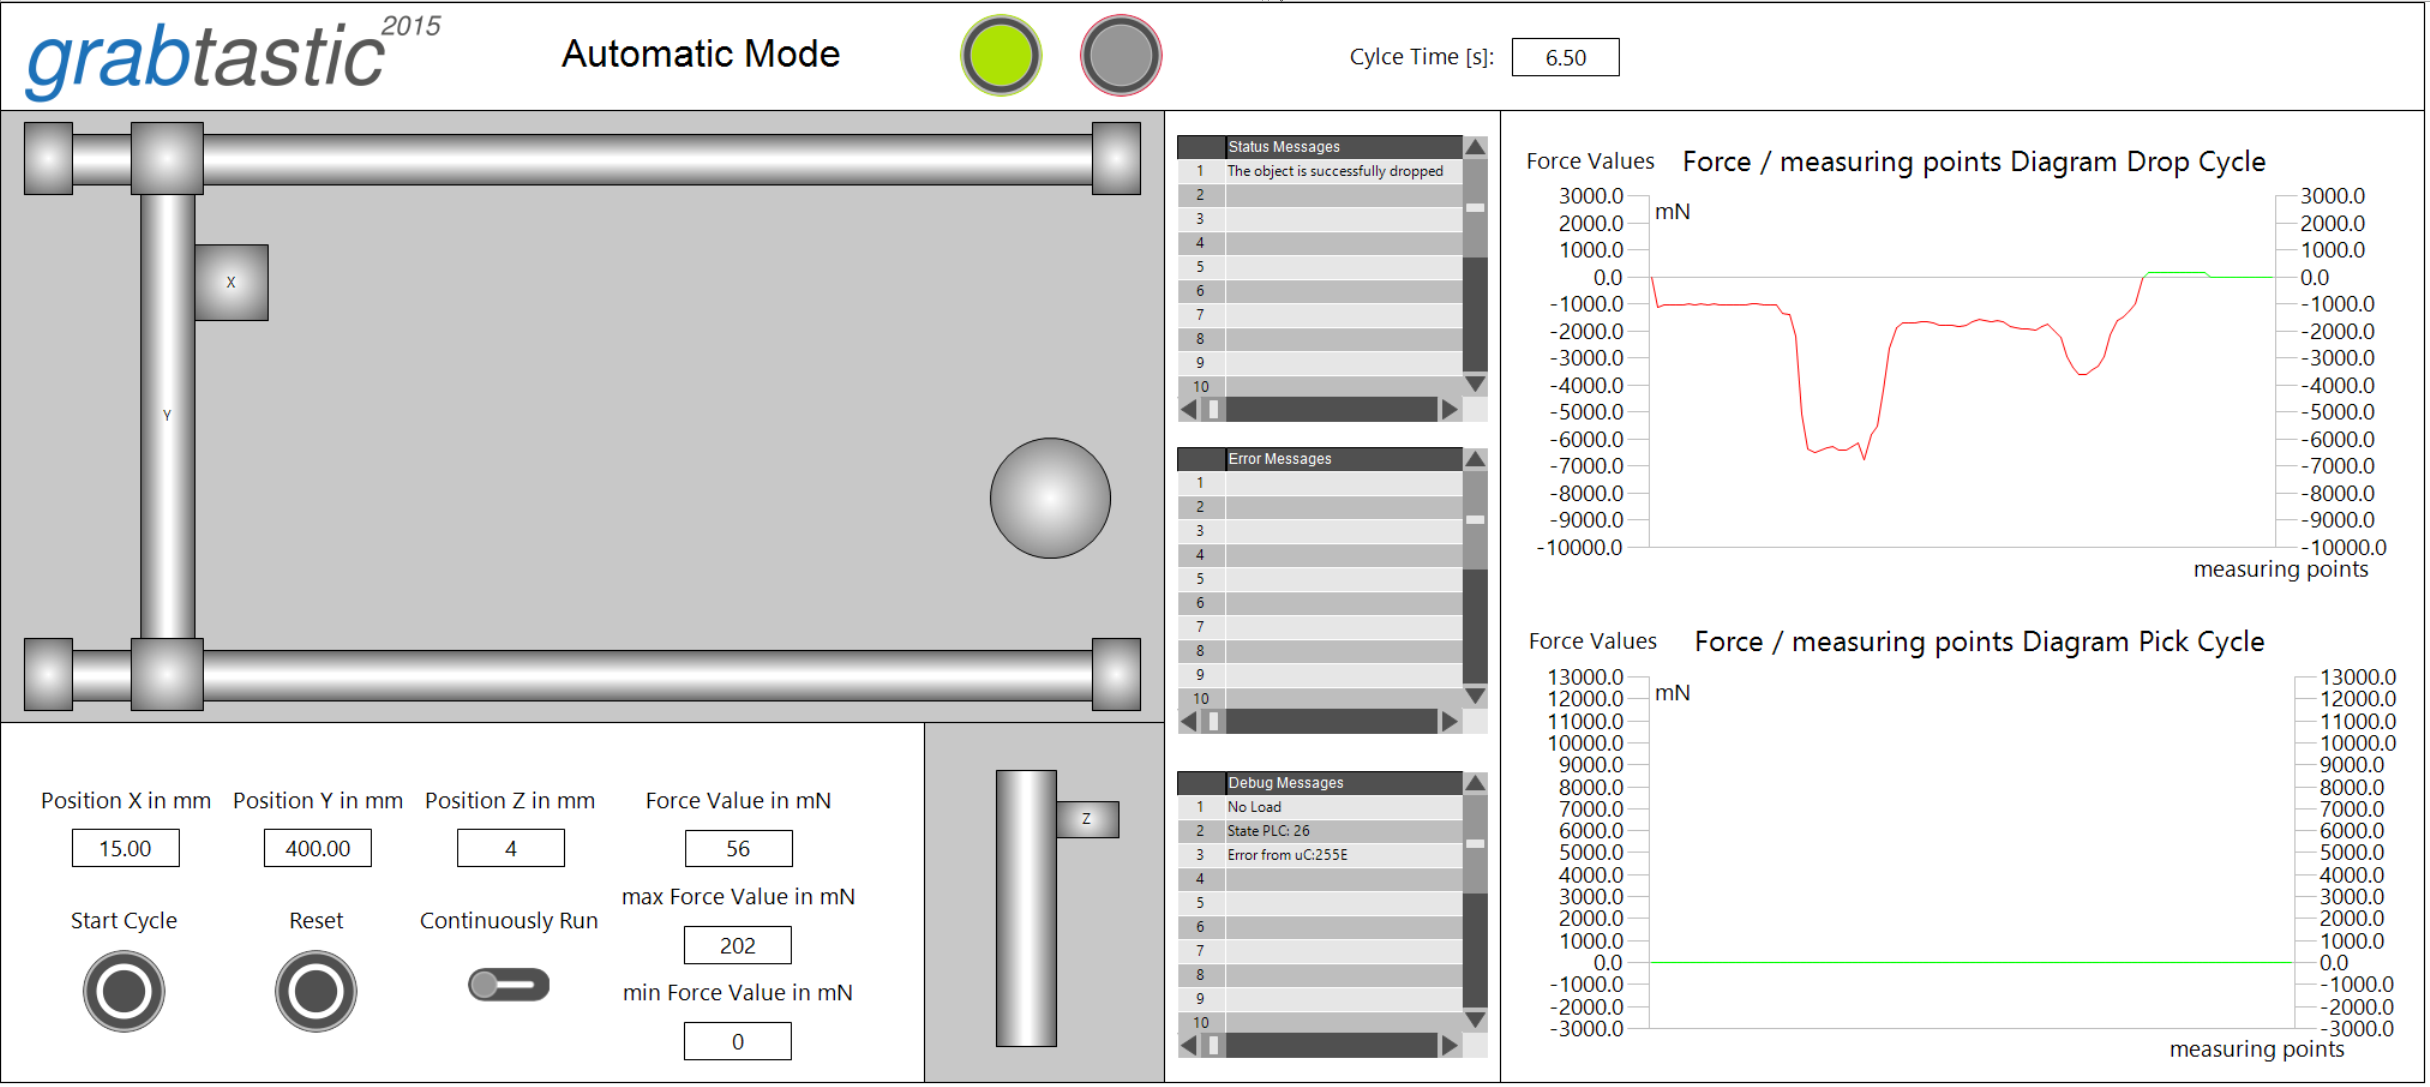
\includegraphics[width=1.4\textwidth]{pictures/automaitk_mode}
   \caption[Automatic mode]{Automatic mode\\
	Source: Group 4}
   \label{fig:automatic mode}
\end{figure} 
\end{landscape}

\chapter{Communication \acs{PLC} - \acs{uC}}

\section{Configuration of \acs{RS232}}\label{sec: config of rs232}

\begin{itemize}
\item $9600 Baud$/$115,2kBaud$ \footnote{both are tested, now its running with $115,2kBaud$}, 8Bit, 1 Stop Bit, no parity, ASCII
\item Master: \acs{PLC}
\item Slave: \acs{uC}
\item Frame: no address, no checksum, delimiter: CR ("\textbackslash r") NL ("\textbackslash n")
\end{itemize}

\section{Commands \acs{PLC}}
\begin{itemize}
\item \acs{I} ... Initialization: axis resets and moves up to to reference point
\item \acs{H} ... Homing: axis moves up to home position
\item \acs{D} ... Down: axis moves down
\item \acs{P} ... Pre Position: axis moves to the pre position
\end{itemize}

\section{Reply \acs{uC}}
 
 \begin{itemize}
\item \acs{ok} ... command accepted
\item \acs{busy} ... command not accepted (e.g. when movement is ongoing)
\item \acs{UNKNOWN} ... command unknown
\item \acs{i} ... when axis is referenced
\item \acs{h} ... when axis has reached home position
\item \acs{d} ... when axis has reached down position
\item \acs{p} ... when axis has reached pre position
\end{itemize}

\section{Telegram from \ac{uC} to \ac{PLC}}\label{sec:telegram plc uc}
The telegram looks like the following:\\
<respond>/<$\#$ force value>/<z-axis position>/<error>\textbackslash r \textbackslash n
\begin{itemize}
\item The delimiter / is used to separate each value.
\item \textbackslash r \textbackslash n are used as suffix.
\item $\#$ to mark the value as force
\end{itemize}

In \autoref{tab: telegram examples} there are examples of the respond from the \acs{uC}. The z-axis is a value in $mm$, the force value is a value in $mN$.

\begin{table}[H]
\centering
\begin{tabular}{|l|c|c|c|c|c|c|c|c|}
\hline 
 respond &  \acs{del} &  $\#$ force value &  \acs{del} &  z-axis position &  \acs{del} &  error & \textbackslash r & \textbackslash n\\ 
 \hline 
 \acs{i} &  / &  $\#$-1000 &  / &  4 & /  &  0E &  \textbackslash r & \textbackslash n \\ 
 \hline 
 \acs{d} &  / & $\#$-1100 &  / &  5 &  / &  0E &   \textbackslash r & \textbackslash n \\ 
 \hline 
 \acs{h} &  / &  $\#$-1200 & / & 6 &  / &  0E &   \textbackslash r & \textbackslash n \\ 
 \hline 
 \acs{p} & / &  $\#$-1300 &  / & 7 &  / &  0E &  \textbackslash r & \textbackslash n \\ 
 \hline 
 \acs{ok} &  / &  $\#$-1400 &  / &  8 &  / &  0E &  \textbackslash r & \textbackslash n \\ 
 \hline 
 \acs{busy} &  / &  $\#$-1500 &  / &  9 &  / &  0E &  \textbackslash r & \textbackslash n \\ 
 \hline 
 \acs{UNKNOWN} &  / &  $\#$2000 &  / &  10 &  / &  0E &   \textbackslash r & \textbackslash n \\
\hline 
\end{tabular} 
\caption{Examples of telegrams}
\label{tab: telegram examples}
\end{table}

\section{Heartbeat}

The value of the Force Sensor is used as the heartbeat, if there is no heartbeat for two second, the communication between the \ac{PLC} and the \ac{uC} is disturbed.

\chapter{\acs{uC} Program}

An Atmel AT-SAM-D20-J18 is used to control the Z-Axis. It has a micro USB connector for programming and debugging and three identical but separate external ports (PWR, EXT1, EXT2, EXT3) for making connections. To program the \acs{uC} the Atmel Studio is used. It bases on Microsoft Visual Studio. The coding guideline from Doxygen\footnote{see at \href{http://www.stack.nl/~dimitri/doxygen/manual/docblocks.html}{Doxygen Documentation}} is used.

  \begin{figure} [H]
        \centering
        \begin{subfigure}[b]{0.45\textwidth}
                \centering
                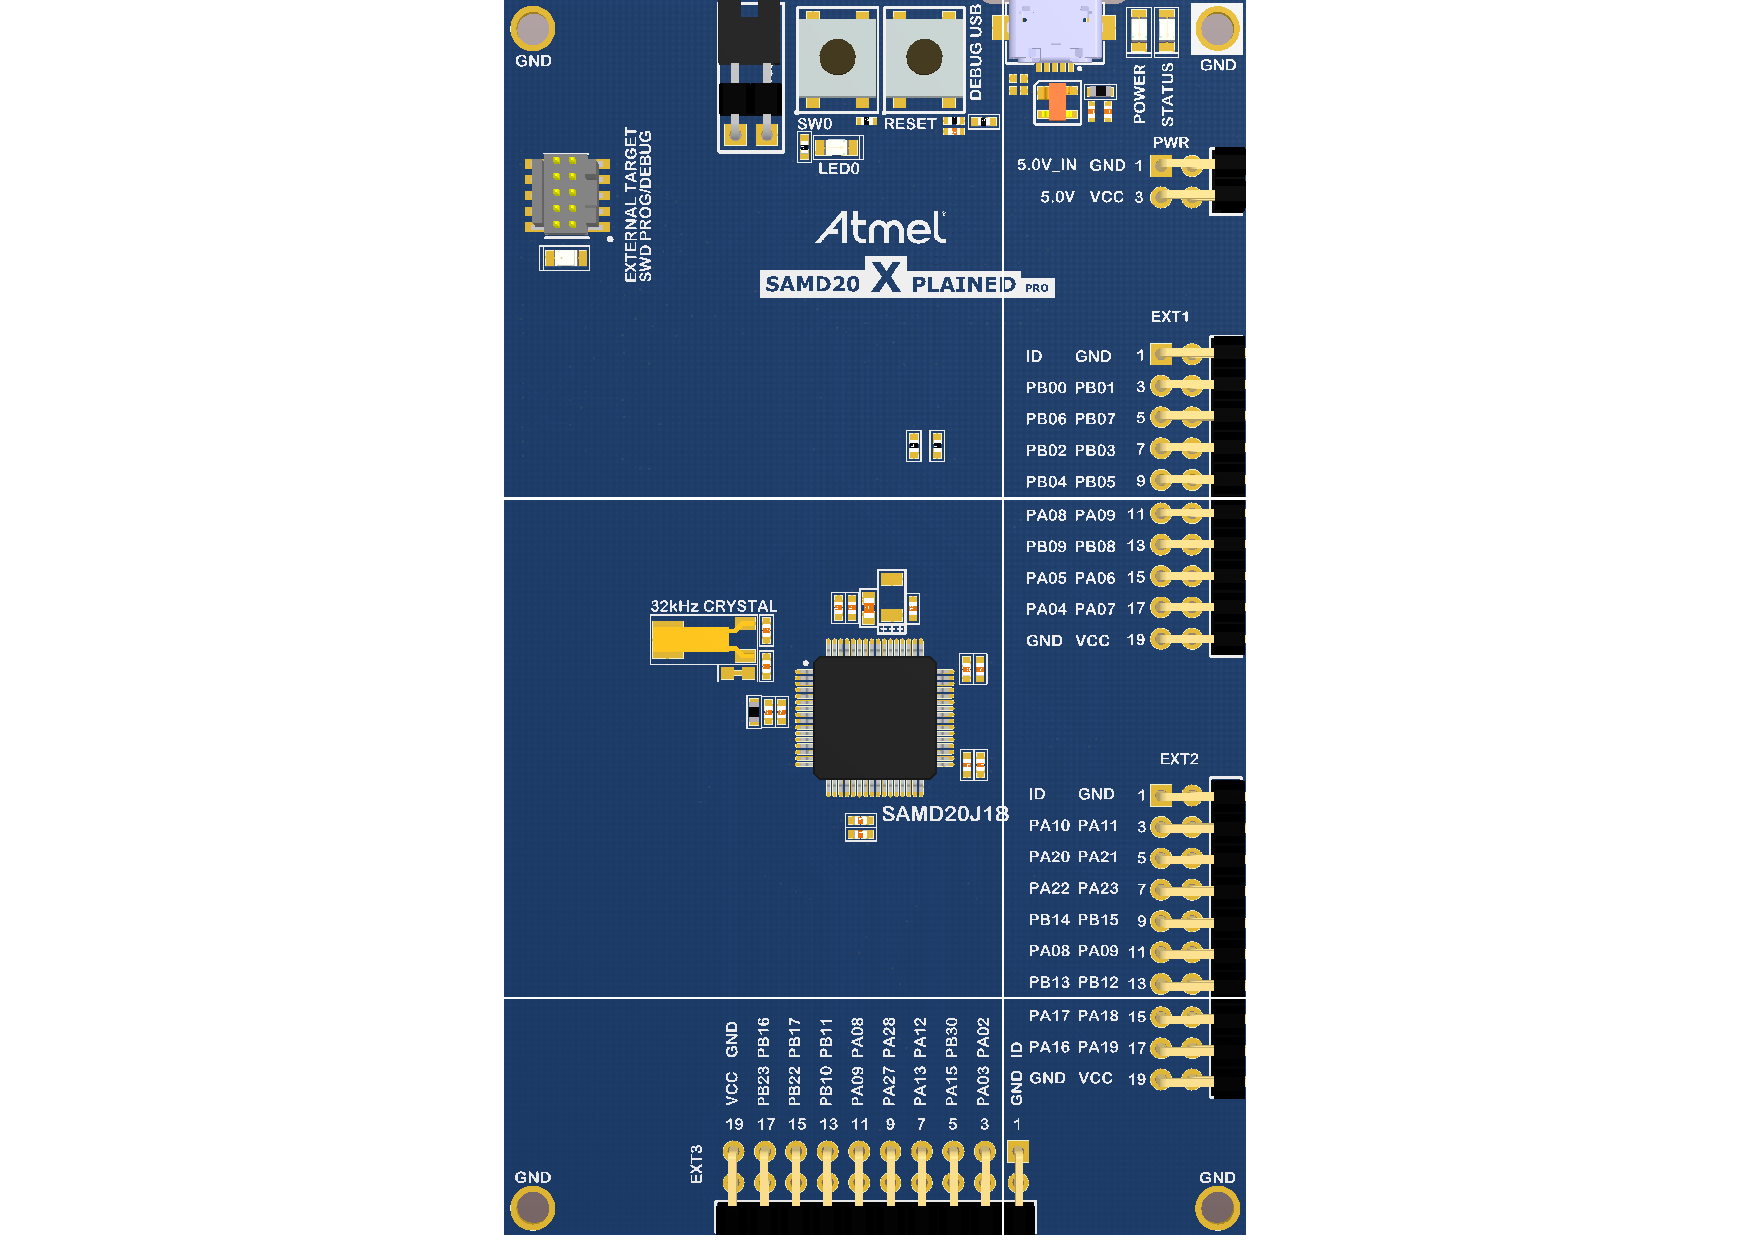
\includegraphics[width=1\textwidth]{pictures/atmel_top.pdf}
                \caption{Top}\label{fig:atmel top}
        \end{subfigure}%
        ~ % An dieser Stelle kann ein zusätzlicher Zwischenraum eingebunden werden: ~, \quad, \qquad, \hfill usw.
          % Eine leere Zeile erzwingt, dass die zweite Grafik darunter erscheint.
        \begin{subfigure}[b]{0.45\textwidth}
                \centering
                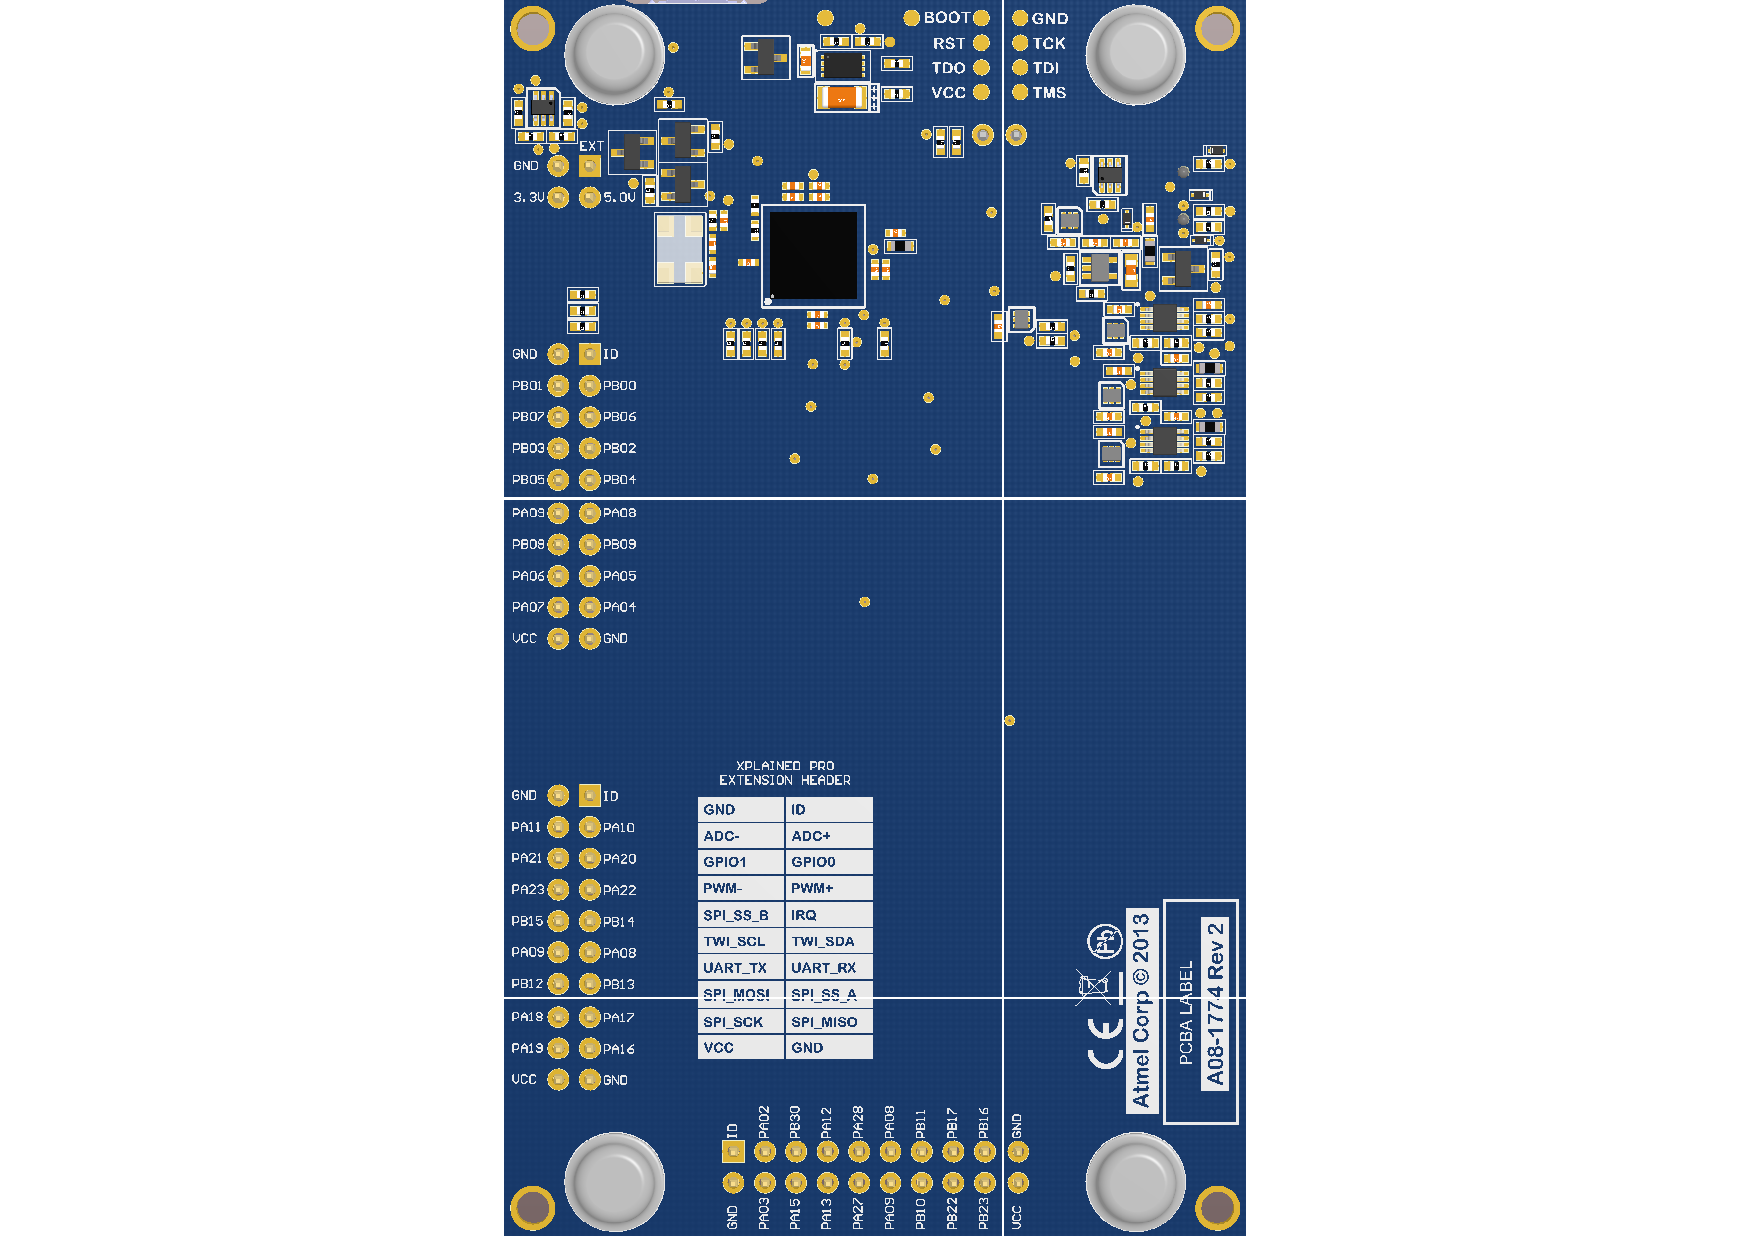
\includegraphics[width=1\textwidth]{pictures/atmel_bottom.pdf}
                \caption{Bottom}\label{fig:atmel bottom}
        \end{subfigure}
        \caption[Top and bottom view of the used atmel board]{Top and bottom view of the used atmel board\\
        Source: Atmel data sheet design documentation, page 10-11}\label{fig:atmel top and bottom}
  \end{figure}

\section{\acs{ASF} Library}
The \acs{ASF} is a collection of free embedded software for Atmel \acs{uC} devices. It simplifies the usage of Atmel products, providing an abstraction to the hardware and high-value middleware. \acs{ASF} is designed to be used for evaluation, prototyping, design and production phases. \acs{ASF} is integrated in the Atmel Studio IDE with a graphical user interface or available as a standalone package for several commercial and open source compilers. The basic structure can be seen in \autoref{fig:asf lib}.

\begin{figure}[H]
  \centering
   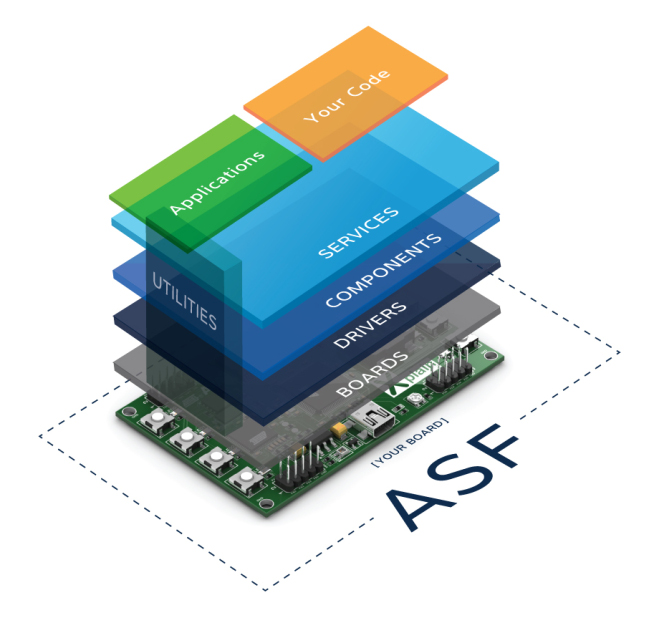
\includegraphics[width=0.5\textwidth]{pictures/ASF}
   \caption[ASF library]{ASF library\\
	Source: Atmel \acs{ASF} Library data sheet 
   }
   \label{fig:asf lib}
\end{figure} 

Used parts of the \acs{ASF}:

\begin{itemize}
\item Generic board support
\item IOPORT - General purpose \acs{I/O} service (service)
\item Delay routines (service, systick)
\item \acs{ADC} (driver, callback\footnote{callback means, that it generates an interrupt request})
\item PORT GPIO Pin Control (driver)
\item SERCOM \acs{SPI}(Master Mode, Vectored \acs{I/O}, driver, callback)
\item SERCOM USART Serial Communications (driver, callback)
\item SYSTEM Power Management (driver)
\item \acs{TC} (driver, callback)
\end{itemize}

\section{Used pins}
In \autoref{fig:EXT1 used pins}, \autoref{fig:EXT2 used pins} and \autoref{fig:EXT3 used pins} are the used pins shown with the functionality.
\begin{table}[H]
\centering
\begin{tabular}{|p{2.5cm}|p{2.8cm}|p{5.8cm}|p{3.5cm}|}
\hline
Pin on EXT1 & SAM D20 pin & Function                                   & Used for            \\ \hline
3           & PB00        & AIN[8]                                     & amplifier \acs{ADC} \\ \hline
9           & PB04        & EXTINT[4]                                  & Emergency Stop      \\ \hline
13          & PB09        & SERCOM4 PAD[1] UART RX1                    & \acs{RS232}         \\ \hline
14          & PB08        & SERCOM4 PAD[0] UART TX1                    & \acs{RS232}         \\ \hline
18          & PA07        & SERCOM0 PAD[3] SPI SCK                     &         Referenc for \acs{ADC}            \\ \hline
19          & -           & GND                                        &                     \\ \hline
20          & -           & VCC                                        &                     \\ \hline
\end{tabular}
\caption{EXT1 used pins}
\label{fig:EXT1 used pins}
\end{table}

\begin{table}[H]
\centering
\begin{tabular}{|p{2.5cm}|p{2.8cm}|p{5.8cm}|p{3.5cm}|}
\hline
Pin on EXT2 & SAM D20 pin & Function                & Used for                 \\ \hline
5           & PA20        & GPIO                    & DRV8711 Sleep            \\ \hline
6           & PA21        & GPIO                    & DRV8711 reset            \\ \hline
7           & PA22        & TC4/WO[0]               & DRV8711 stepping frequency        \\ \hline
9           & PB14        & EXTINT[14]              & DRV8711 change direction \\ \hline
15          & PA17        & SERCOM1 PAD[1] SPI SS   & DRV8711 \acs{SPI}            \\ \hline
16          & PA18        & SERCOM1 PAD[2] SPI MOSI & DRV8711 \acs{SPI}              \\ \hline
17          & PA16        & SERCOM1 PAD[0] SPI MISO & DRV8711 \acs{SPI}              \\ \hline
18          & PA19        & SERCOM1 PAD[3] SPI SCK  & DRV8711 \acs{SPI}             \\ \hline
19          & -           & GND                     &                          \\ \hline
20          & -           & VCC                     &                         \\ \hline
\end{tabular}
\caption{EXT2 used pins}
\label{fig:EXT2 used pins}
\end{table}

\begin{table}[H]
\centering
\begin{tabular}{|p{2.5cm}|p{2.8cm}|p{5.8cm}|p{3.5cm}|}
\hline
Pin on EXT2 & SAM D20 pin & Function  & Used for     \\ \hline
9           & PA28        & EXTINT[8] & Limit switch \\ \hline
19          & -           & GND       &              \\ \hline
20          & -           & VCC       &              \\ \hline
\end{tabular}
\caption{EXT3 used pins}
\label{fig:EXT3 used pins}
\end{table}

\newpage
\section{Configuration}\label{sec:config_uc}
For the needs you see in \autoref{fig:electronic System Overview} following configuration\footnote{Configuration uses different parts of the \acs{ASF} library} at the \acs{uC} is necessary:
\begin{enumerate}
\item\textbf{ \acs{ADC}} 
\begin{itemize}
\item clock generator 2 (3$2kHz$)
\item a clock prescaler of 4
\item uses the reference B
\item the resolution is set to 10 bit
\end{itemize}
\item \textbf{\acs{TC}}
\begin{itemize}
\item is configured with clock generator 0 ($8MHz$)
\item a counter size of 16 bit's
\item the wave generation is frequency match mode
\item The compare value is moving between $9500$ and $7600$.
\end{itemize}
\item \textbf{\acs{RS232}}
\begin{itemize}
\item Is configured with a baudrate of $9600$ like it is mentioned in \autoref{sec: config of rs232}
\item on EXT1
\end{itemize}
\item \textbf{\acs{SPI}}
\begin{itemize}
\item Is configured with the standard values given from the \acs{ASF} library
\item It has a baudrate of $100000$ as you can be seen in  \autoref{fig:SPI_send_config_measurement} and \autoref{fig:SPI_send_status_measurement}
\end{itemize}
\item \textbf{External interrupt}\\
Two external interrupt are configured, one for the emergency and one for the limit switch. Both has the following configuration:
\begin{itemize}
\item Pull down resistor
\item detect both signal edges (limit switch) and detect falling edges (emergency)
\item filtering input signal is enabled
\end{itemize}
\item\textbf{ \acs{I/O}'s}
\begin{itemize}
\item all has a pull down resistor
\item as output
\item Pin 5, 6 and 9 are activated
\end{itemize}
\end{enumerate}

\section{Calculations}

\subsection{Sampling Rate of the \acs{ADC}}

\begin{eqnarray}
f&=&\frac{clock \, generator \, 2}{prescaler}\\
f&=&\frac{32*10^{3}Hz}{4}=8000Hz
\end{eqnarray}

With the reciprocal value the sampling rate is calculated.

\begin{eqnarray}
\frac{1}{f}&=&\frac{1}{8000Hz}\\
\frac{1}{f}&=&0,000125s=0,125ms
\end{eqnarray}

$0,125ms$ are fast enough to measure the force.

\subsection{\acs{TC} Frequency}
With the values mentioned in \autoref{sec:config_uc} leads us to the following frequencies, which is the stepping frequency of the DRV8711.
\begin{eqnarray}
f_{out} &=& \frac{f_{0}}{compare \, Value *2}\\
f_{out} &=& \frac{8*10^{6}Hz}{9500*2}=421Hz\label{eq:frequency1}\\
f_{out} &=& \frac{8*10^{6}Hz}{7600*2}=526Hz\label{eq:frequency2}
\end{eqnarray}

\section{Main Loop}


In \autoref{fig:Mainprogramm.pdf} the loop of the main program is shown according to the \acs{UML} standards.
\begin{figure}[H]
  \centering
   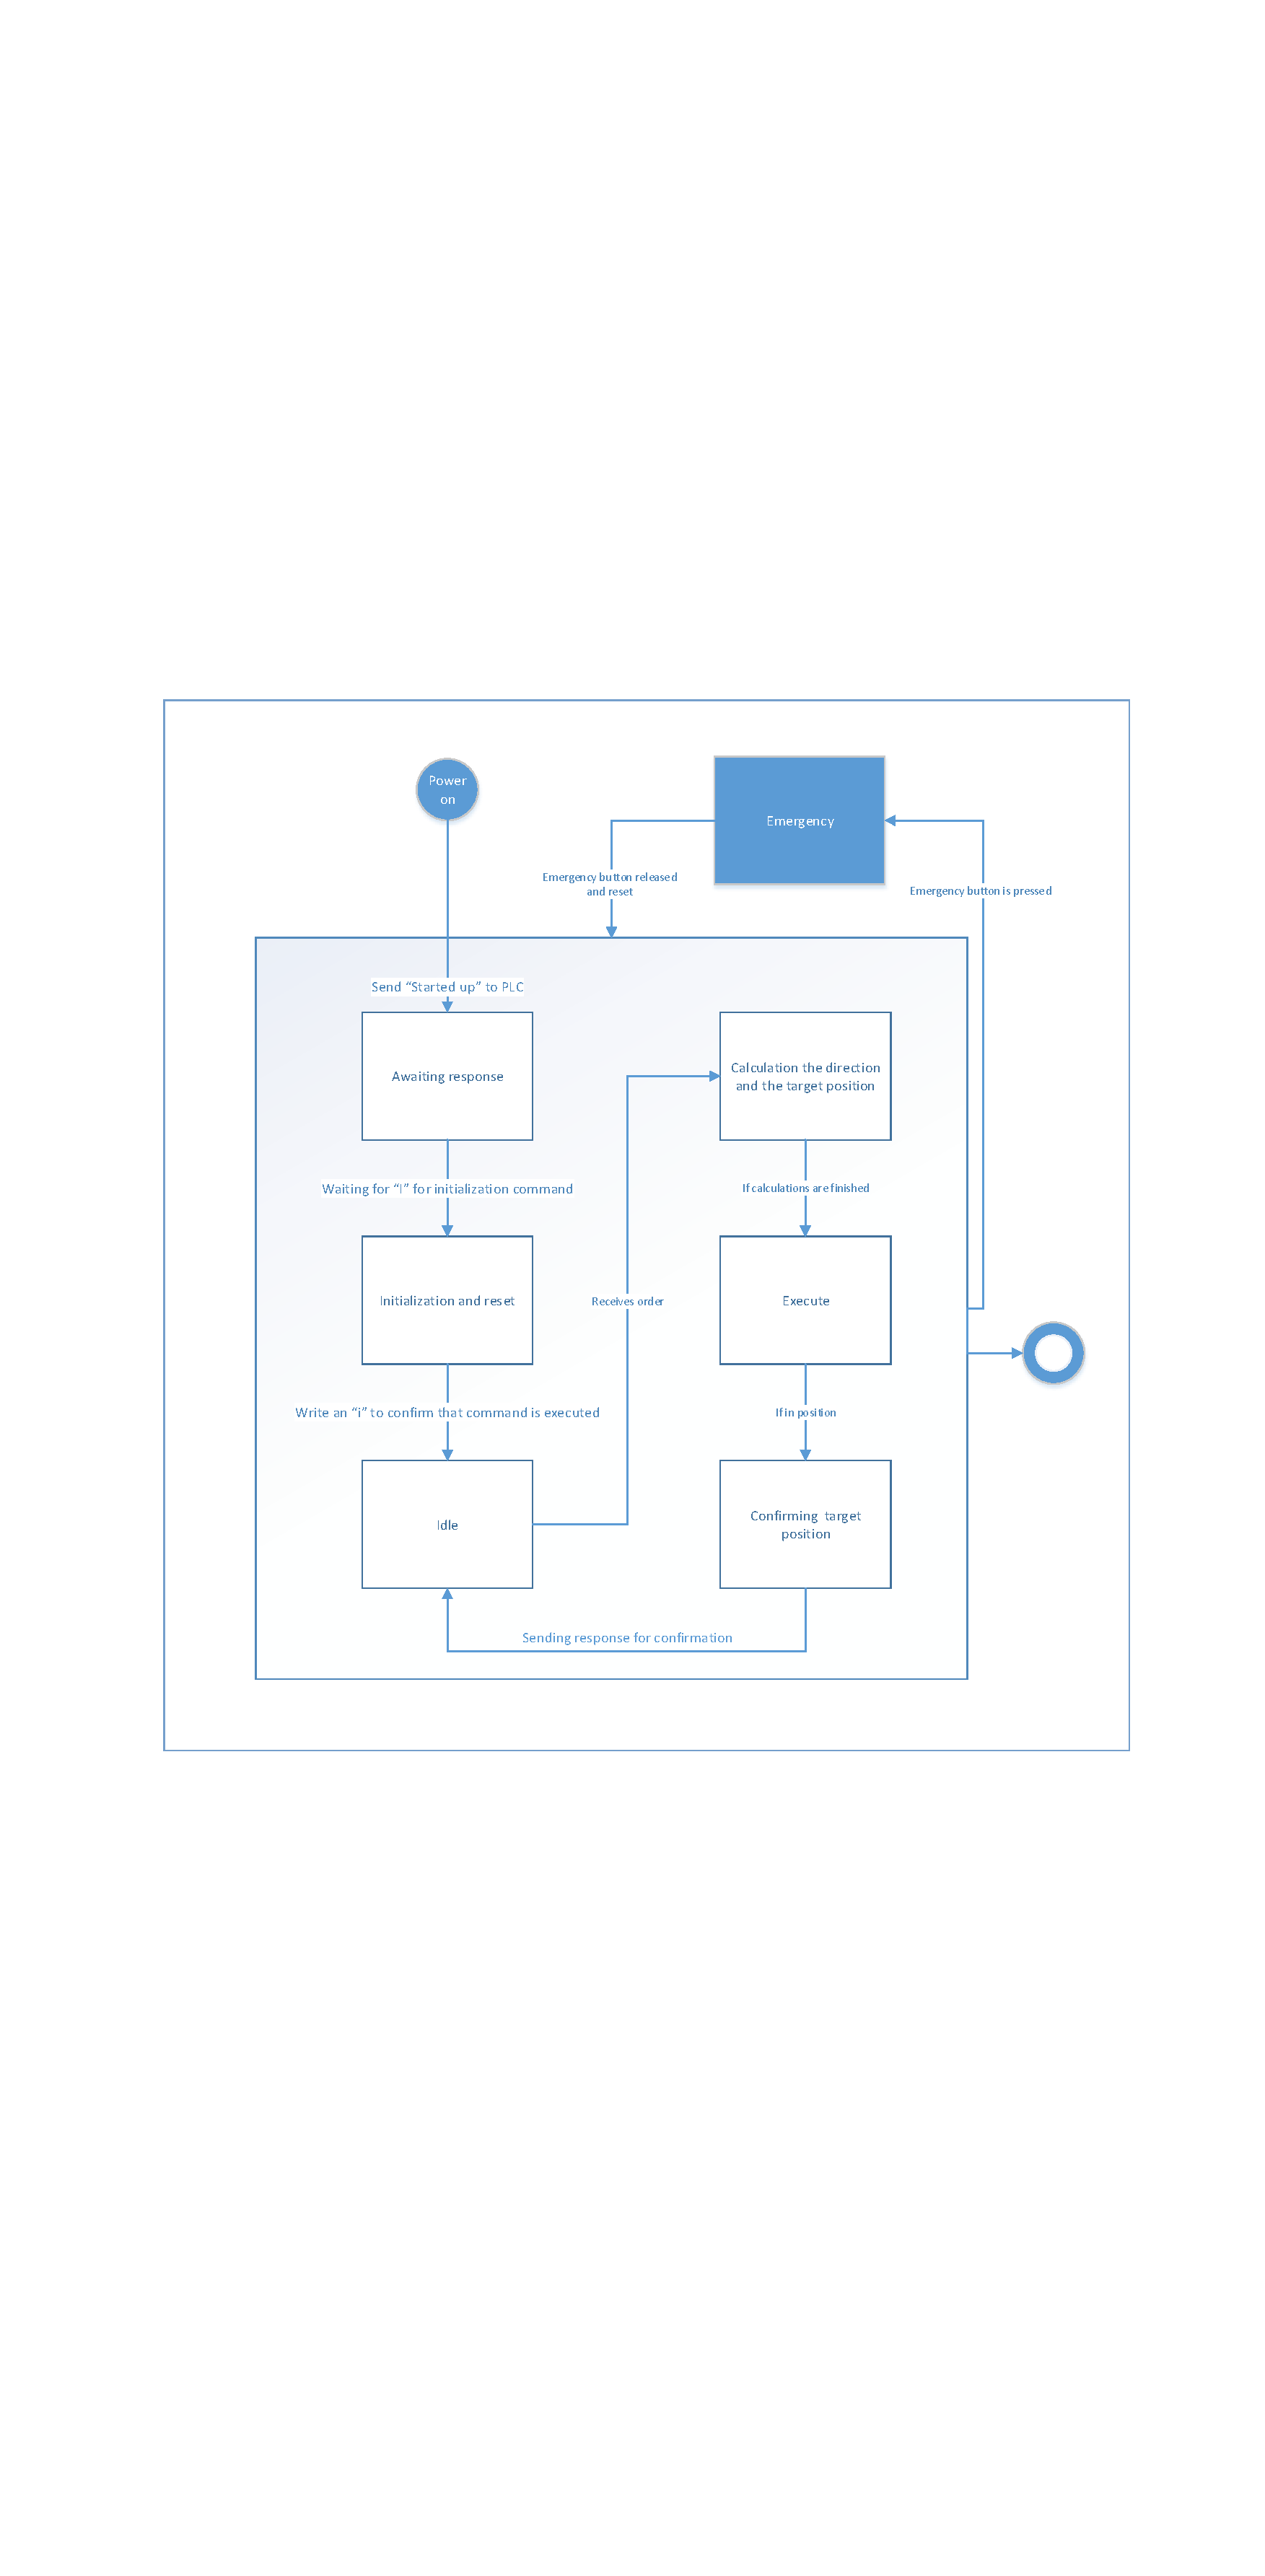
\includegraphics[width=1\textwidth]{pictures/Mainprogramm.pdf}
   \caption[UML Diagram \acs{uC}]{UML Diagram \acs{uC}\\
	Source: Group 4  
   }
   \label{fig:Mainprogramm.pdf}
\end{figure} 
\section{Programmed Functions}

\autoref{fig:h dateien} shows the included header files.

\begin{figure}[H]
  \centering
   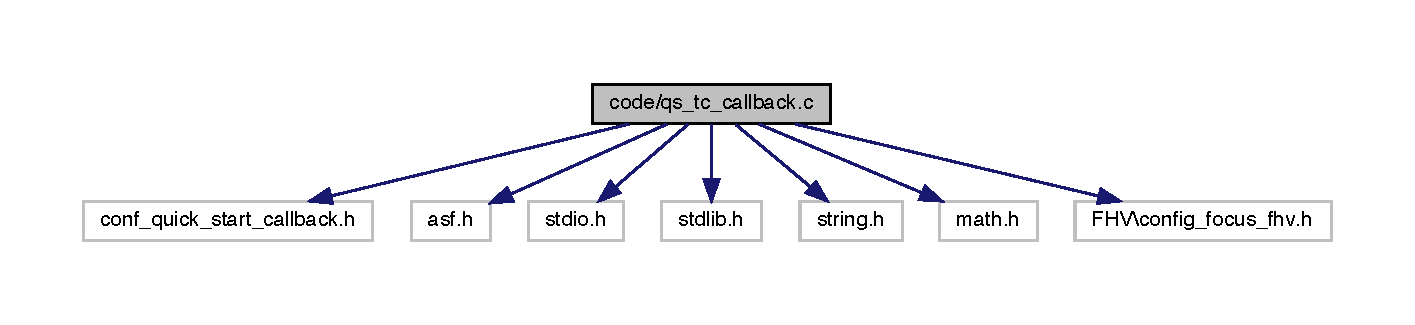
\includegraphics[width=1\textwidth]{pictures/hDateien.pdf}
   \caption[included header files]{Included header files\\
	Source: Group 4  
   }
   \label{fig:h dateien}
\end{figure} 
The config$\_$focus$\_$fhv.t is developed by us. The callgraph of the main loop is shown in \autoref{fig:main call graph program}. The following points describes the process:
\begin{enumerate}
\item configuration is loaded (\autoref{sec:config_uc})
\item main loop starts
\item start a request to read the receive buffer of \acs{RS232}
\item if an order is received, calculate position of the target and direction and start executing it
\item repositioning if we are in the limit switch in case of referencing (order was \enquote{\acs{I}})
\item finish the order
\item start repositioning if the order was a \enquote{\acs{D}}
\item send the telegram, every time a \acs{ADC} measurement is finished
\begin{enumerate}
\item error handling
\item prepare the telegram\footnote{the telegram is mentioned in \autoref{sec:telegram plc uc}} for sending
\item start a request to send the write buffer of \acs{RS232}
\item start a new \acs{ADC} measurement
\end{enumerate}
\end{enumerate}

The positions of the Z-axis are easily expandable if necessary. There is an array of struct, where the positions can be added with the belonging command form the \acs{PLC}.

\begin{figure}[H]
  \centering
   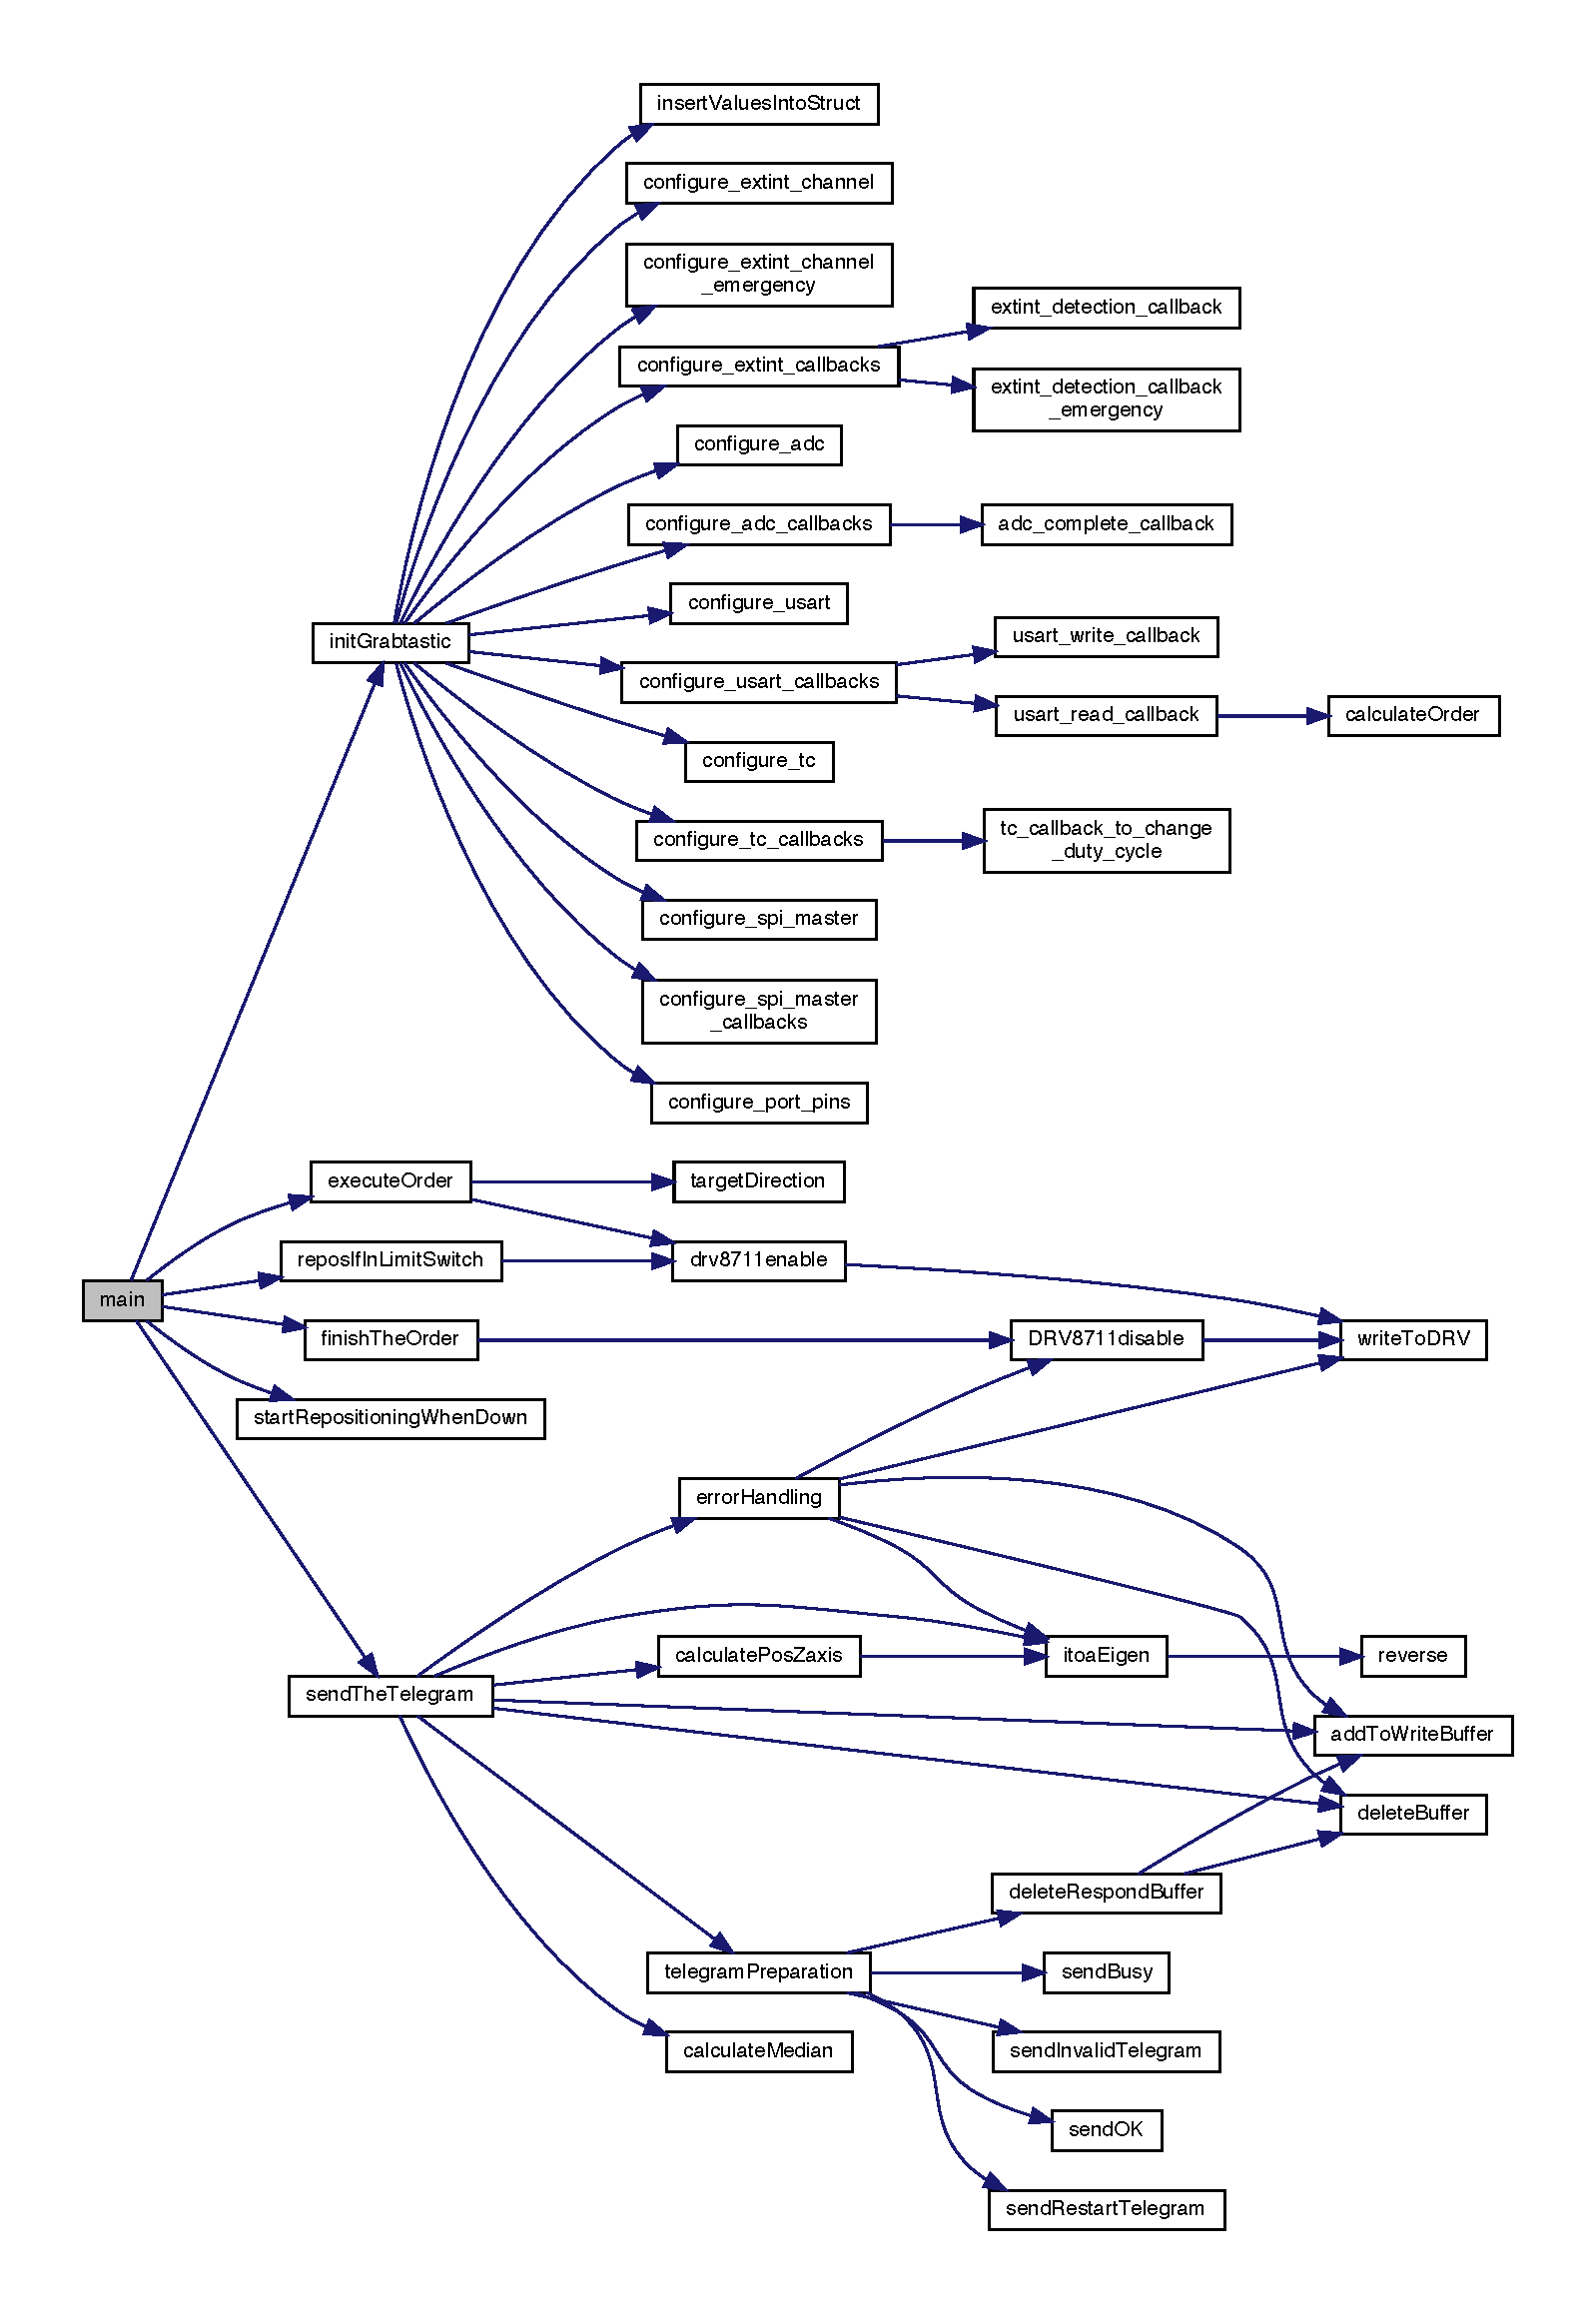
\includegraphics[width=0.85\textwidth]{pictures/main_callgraph.pdf}
   \caption[Called functions \acs{uC}]{Called functions \acs{uC}\\
	Source: Group 4  
   }
   \label{fig:main call graph program}
\end{figure}

\section{DRV8711 Register Settings}\label{DRV8711 register settings}

In \autoref{fig:DRV8711 registers} the adjusted values for the DRV8711 are shown.

  \begin{figure} [H]
        \centering
        \begin{subfigure}[b]{0.85\textwidth}
                \centering
                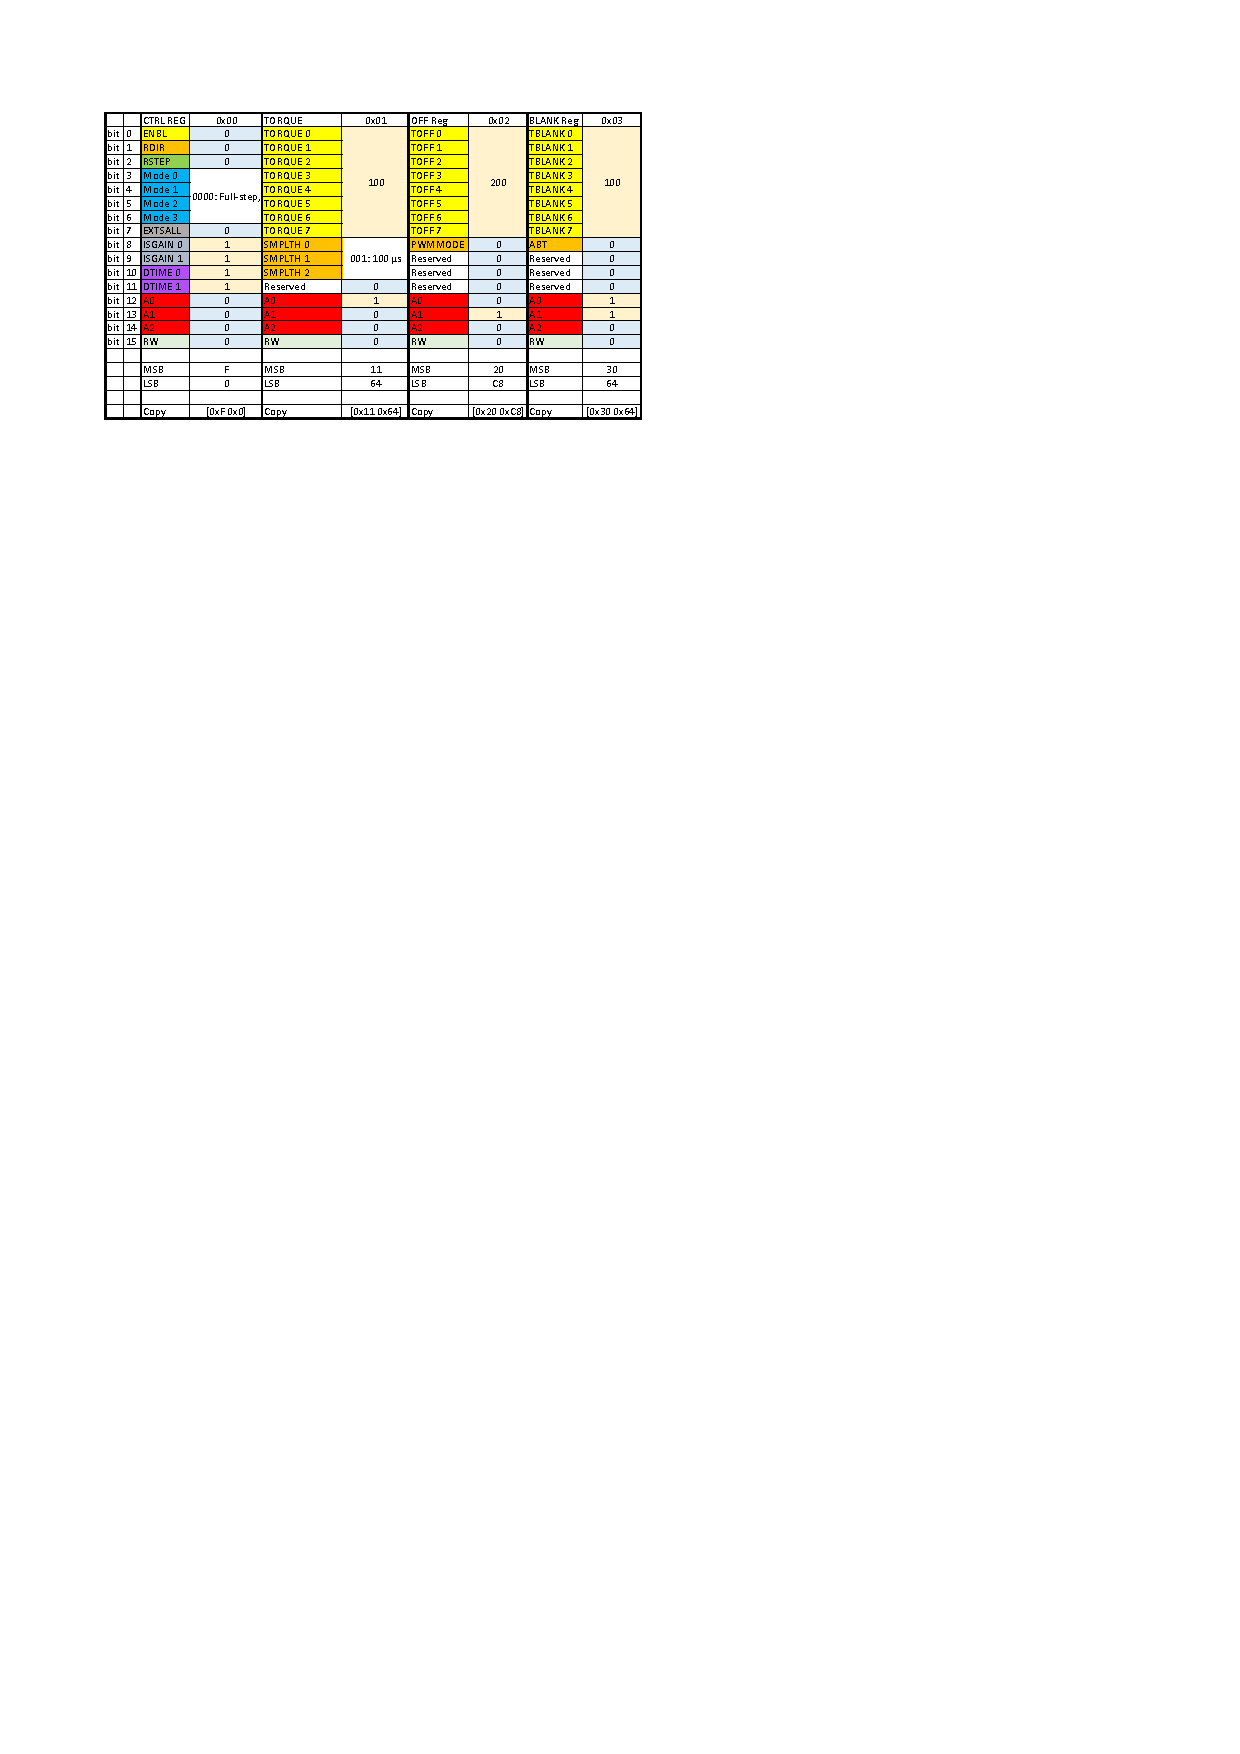
\includegraphics[width=1\textwidth]{pictures/spi_v0_0_1.pdf}
                \caption{Register 0-3}\label{fig:register 0-4}
        \end{subfigure}%
        ~ % An dieser Stelle kann ein zusätzlicher Zwischenraum eingebunden werden: ~, \quad, \qquad, \hfill usw.
          % Eine leere Zeile erzwingt, dass die zweite Grafik darunter erscheint.
          
        \begin{subfigure}[b]{0.85\textwidth}
                \centering
                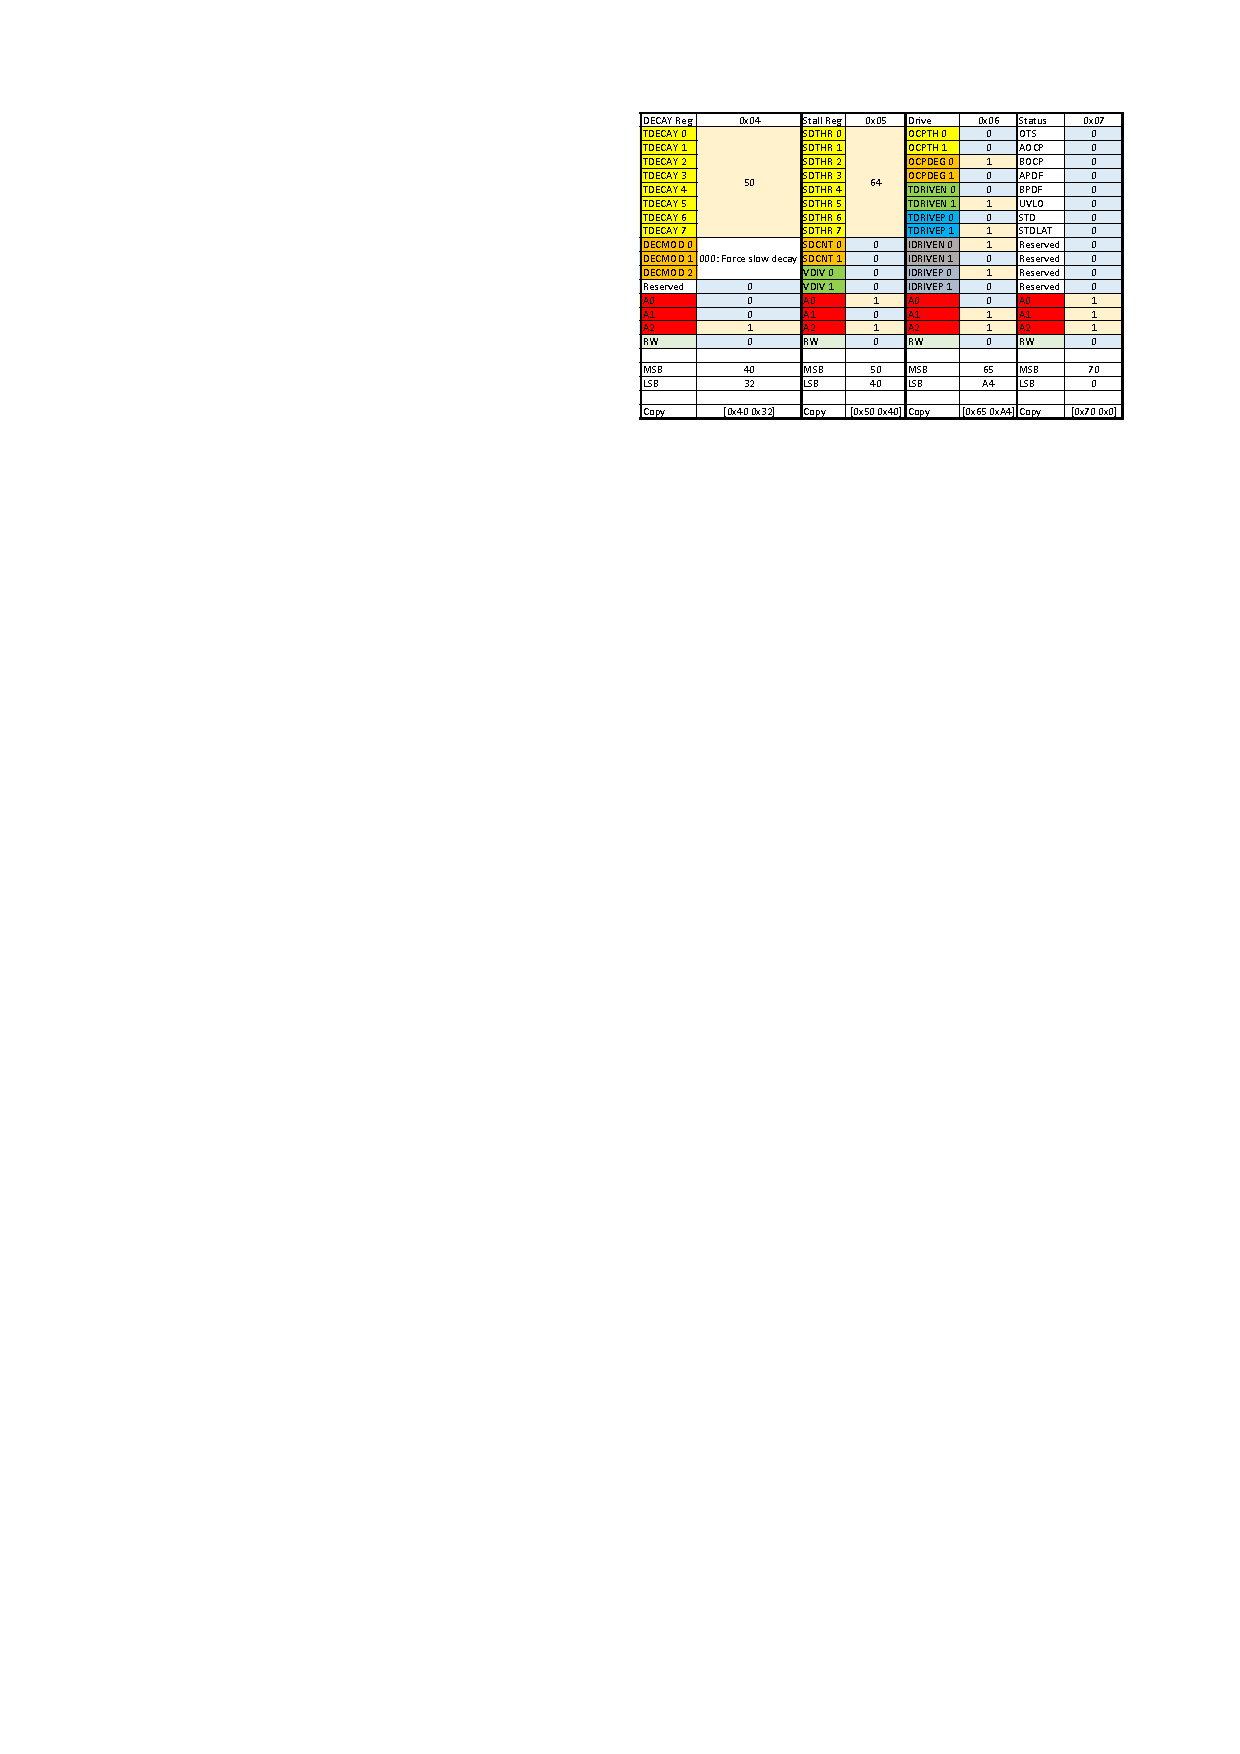
\includegraphics[width=1\textwidth]{pictures/spi_v0_0_2.pdf}
                \caption{Register 4-7}\label{fig:register 5-8}
        \end{subfigure}
        \caption[DRV8711 \acs{PCB} Registers]{DRV8711 \acs{PCB} Register \\
         Source: Group 4}\label{fig:DRV8711 registers}
  \end{figure}

There are eight registers \footnote{detailed description of each register is found at the data sheet of DRV8711 on page 25-28}, seven to configure and one status register. 

\begin{enumerate}
\item [0] CTRL Register is used to enable the H-bridge, set direction, the stepping mode, ISGAIN and DTIME
\item [1] TORQUE Register is used to set the TORQUE and SMPLTH
\item [2] OFF Register is used to set TOFF and PWMMODE
\item [3] BLANK Register is used to set TBLANK and ABT
\item [4] DECAY Register is used to set TDECAY and DECMOD
\item [5] STALL Register is used to set STDHR, SDCNT and VDIV
\item [6] DRIVE Register is used to set OCPTH, OCPDEG, TDRIVEN, TDRIVEP, IDRIVEN and IDRIVEP
\item [7] STATUS register is used to read the status of the DRV8711
\end{enumerate}

\subsection{Configuring Predrivers}
$Q=30nC$\\
$RS=63ns$
\begin{eqnarray}
IDRIVE &>& \frac{Q}{RT} \label{eq: idrive}\\
IDRIVE &>& \frac{30nC}{63ns}\\
IDRIVE &>&  476,2 mA \label{eq: idrive result}\\
TDRIVE &>& 2 * RT \label{eq: tdrive}\\
TDRIVE &>& 2 * 63ns\\
TDRIVE &>& 126ns \label{eq: tdrive result}
\end{eqnarray}
$Q...capacitor \, charge$\\
$RT...rise time$\\
For best results, the smallest IDRIVE and TDRIVE has to be selected. Consequently, according to the data sheet \footnote{DRV8711 page 27-28}, with \autoref{eq: idrive result} the IDRIVE has to be adjusted to the highest value ($IDRIVEN=400mA$, $IDRIVEP=200mA$) and with \autoref{eq: tdrive result} the TRIVE has to be adjusted to $250ns$ ($TRIVEN \, and \, TRIEVEP=250ns$)

\subsection{External \acs{MOSFET}'s calculation}
With the following values the DRV8711 is driving smooth.\\
$DTIME=850 ns$\\
$TBLANK=100 \mu s$\\
$TOFF=200 \mu s$
$Q=30nC$
\begin{eqnarray}
Q&<&\frac{20mA*(2*DTIME+TBLANK+TOFF)}{4}\label{eq:mosfet calc}\\
Q&<&\frac{20mA*(2*0,850\mu s+100\mu s+200\mu s)}{4}\\
Q&<&1508,5nC\label{eq:mosfet calc result}
\end{eqnarray}
With the \autoref{eq:mosfet calc result} we see, that the configuration will work with the IRF520.

\subsection{Speed Calculation}

\begin{eqnarray}
f_{steps} \, \mu steps /s &=& \frac{v*360^{\circ}*n_{m}}{60s/min*\phi \, ^{\circ}/step}\\
\rightarrow v &=& \frac{60 s / min*\phi \, ^{\circ}/step * f_{steps} \, \mu steps /s}{360^{\circ}*n_{m}}
\end{eqnarray}
$v ... rotations/min$\\
With following values the rotational speed is calculated\footnote{found in the motor data sheet and \autoref{eq:frequency1}, \autoref{eq:frequency2}}\\
$\phi =1,8^{\circ}/step$\\
$k=1,5 mm/rot \, pitch \, trapez \, thread$\\
$n_{m}=1$\\
$f_{steps \, 1} = 421Hz$\\
$f_{steps \, 2} = 526Hz$
\begin{eqnarray}
n_{1} &=& \frac{60 s / min * 1,8 \, ^{\circ}/step * 421 \, \mu steps /s}{360^{\circ}*1}=126,3 \, rot/min\\
n_{2} &=& \frac{60 s / min * 1,8 \, ^{\circ}/step * 421 \, \mu steps /s}{360^{\circ}*1}=157,9 \, rot/min
\end{eqnarray}

\begin{eqnarray}
v &=& \frac{n}{k}\\
v_{1} &=& 126,3rot/min*1,5mm/rot\\
v_{1} &=& 189,47 mm/min\\
v_{2} &=& 157,9rot/min*1,5mm/rot\\
v_{2} &=& 236,84 mm/min
\end{eqnarray}

With the results, we see that one cycle takes about $22$ seconds, with a stroke of $80mm$.

\subsection{Conclusion DRV8711}
The discerning reader will also have noticed that the register settings did not match the calculations. The reason therefore is, that the motor is not turning smooth with the calculated values. We had to change them to our needs.

\chapter{Results}


At the moment of handing in this document the project is in the following state:
\begin{itemize}
\item Mechanics: done
\item Electronics:  done
\item Software: \acs{PLC} up and running, communication between \acs{uC} and \acs{PLC} working, \acs{ADC} is working
\end{itemize}

%\section{Problems with mechanical construction}

%\section{Problems with \acs{PLC}}

%\section{Problems with \acs{uC}}

\section{Test runs}
The system runs as described in the requirements document.

\section{Mechanic}
In \autoref{fig:mechanic assembly} the finished Z-axis is shown.
  \begin{figure} [H]
        \centering
        \begin{subfigure}[b]{0.45\textwidth}
                \centering
                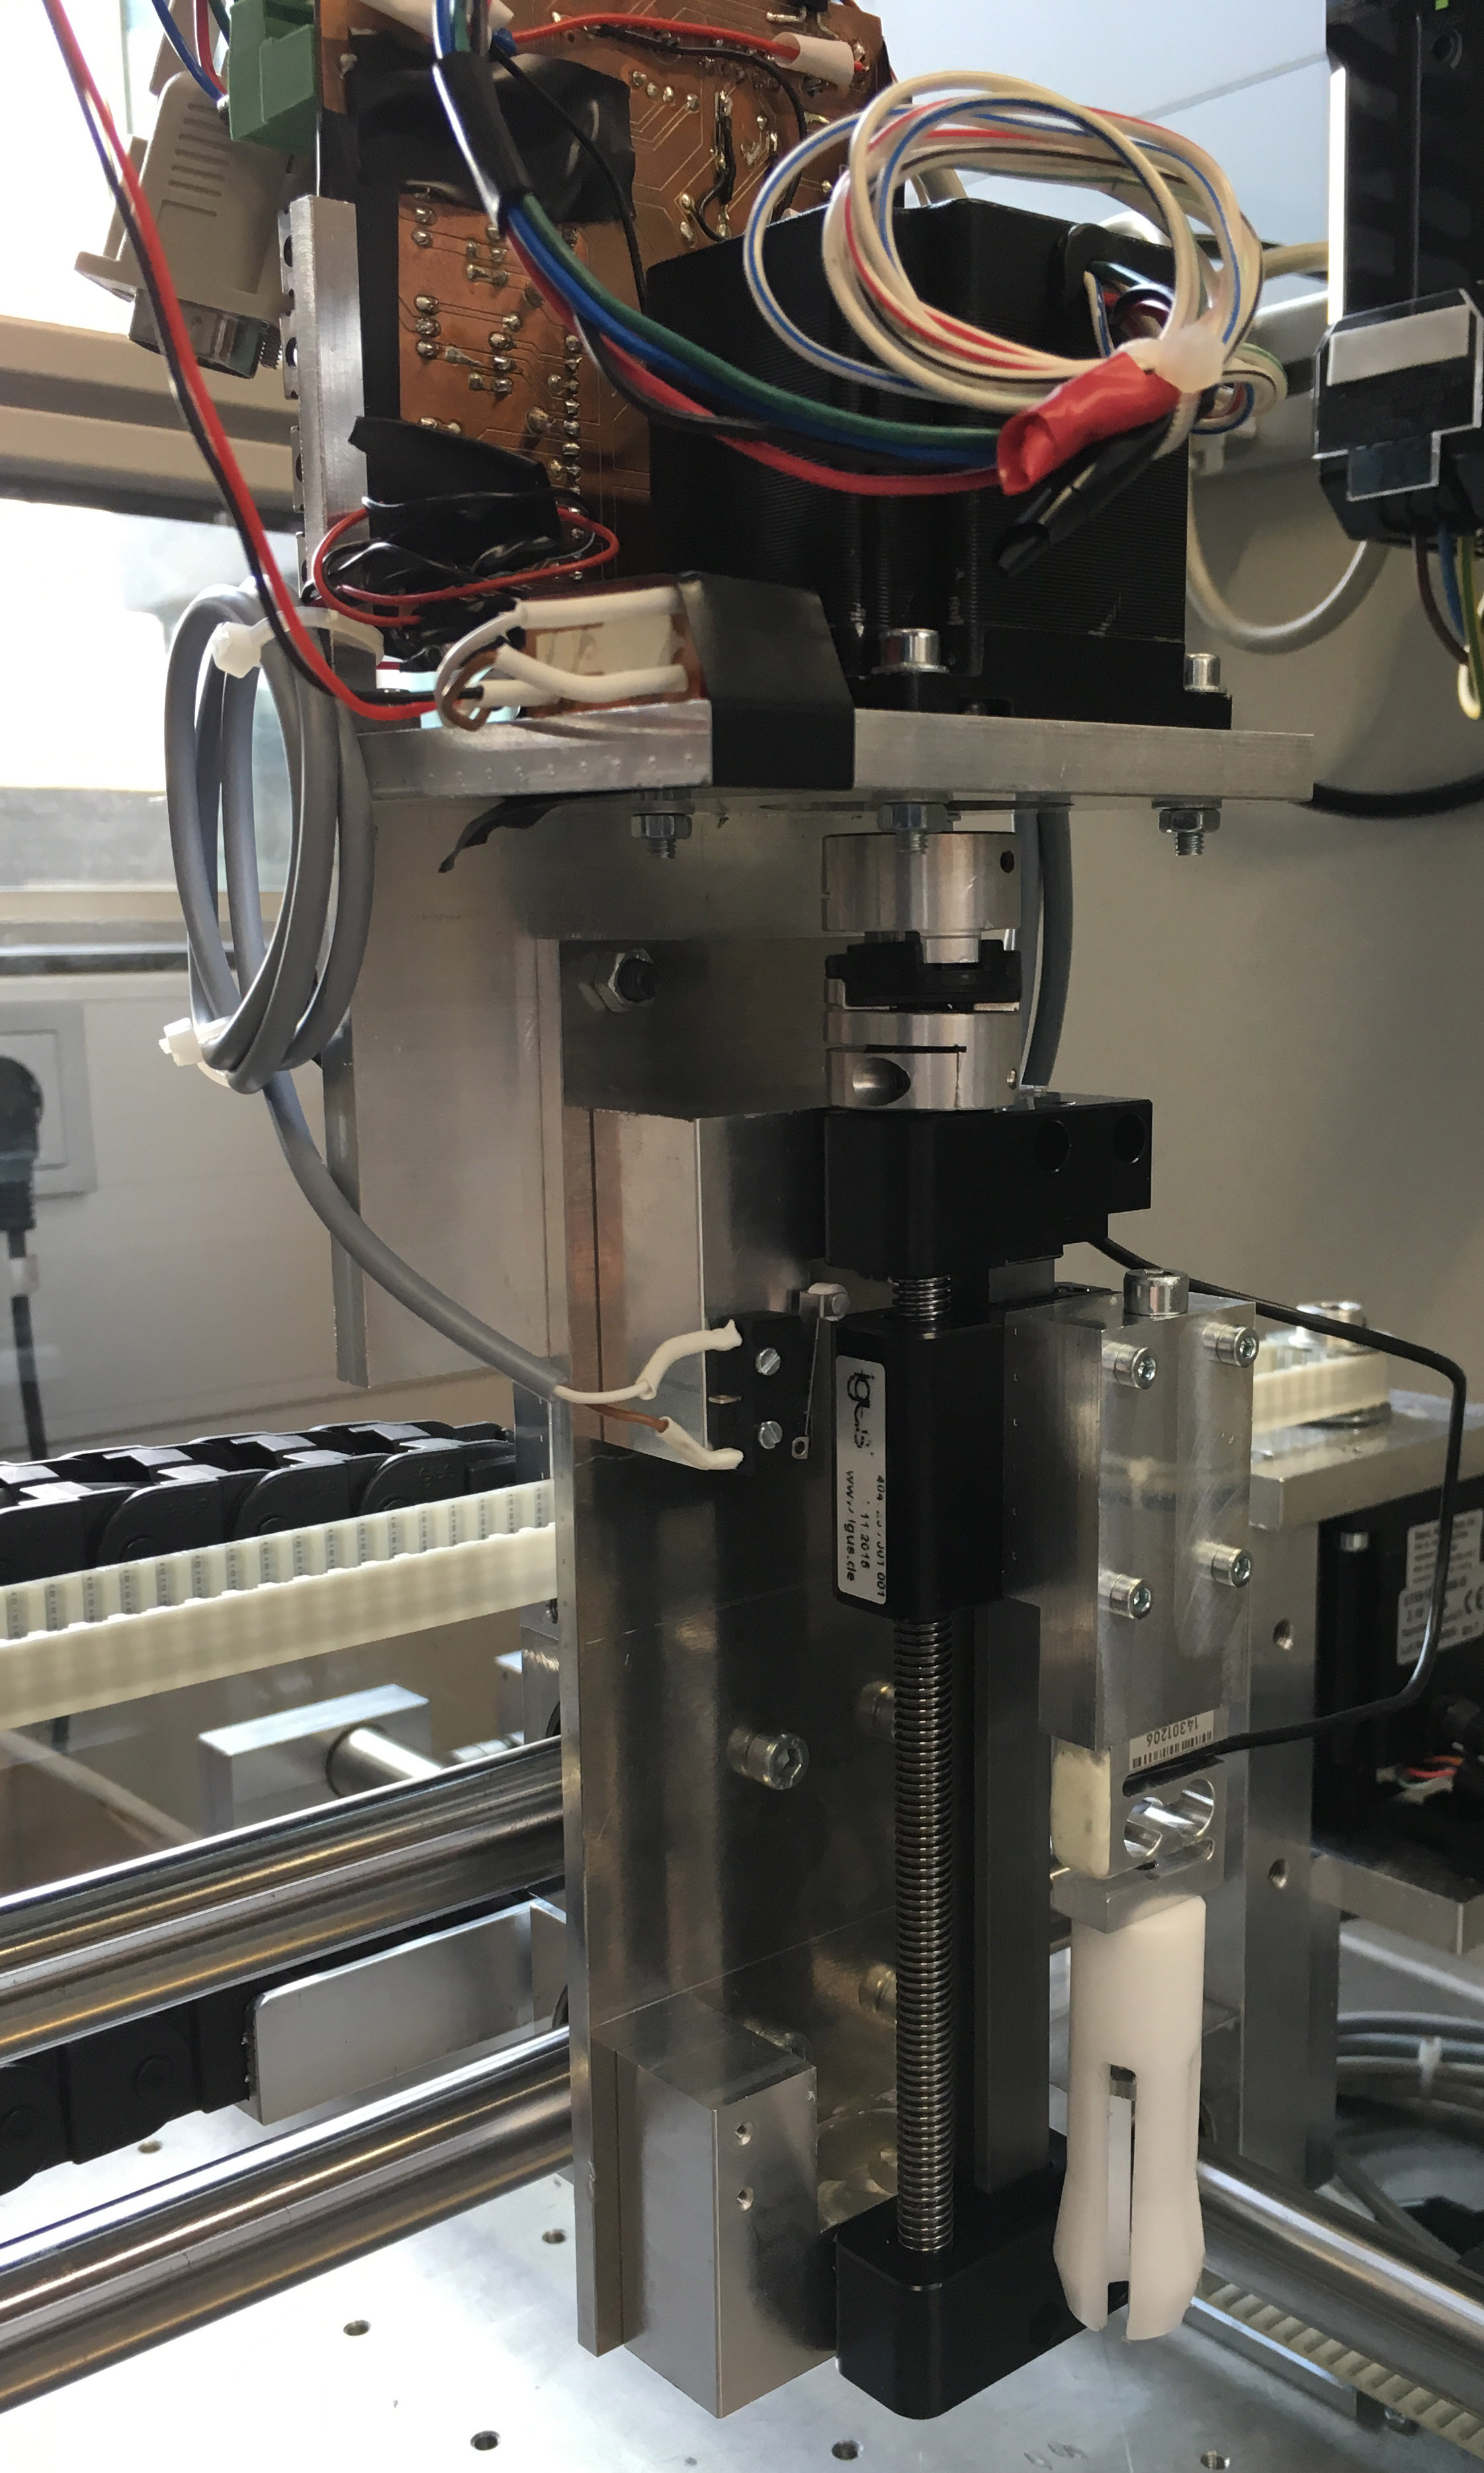
\includegraphics[width=1\textwidth]{pictures/Seitl_1}
              %  \caption{mechanic assembly}\label{fig:Seitl_1}
        \end{subfigure}%
        ~ % An dieser Stelle kann ein zusätzlicher Zwischenraum eingebunden werden: ~, \quad, \qquad, \hfill usw.
          % Eine leere Zeile erzwingt, dass die zweite Grafik darunter erscheint.
        \begin{subfigure}[b]{0.45\textwidth}
                \centering
                \includegraphics[width=0.981\textwidth]{pictures/Seitl_2}
               % \caption{register 4-7}\label{fig:Seitl_2}
        \end{subfigure}
        \caption[Mechanic assembly]{Mechanic assembly\\
         Source: Group 4}\label{fig:mechanic assembly}
  \end{figure}
  \newpage
   In \autoref{fig:rep_side_view} and \autoref{fig:rep_top_view} is the finished \acs{Repository} shown.
  \begin{figure}[H]
  \centering
   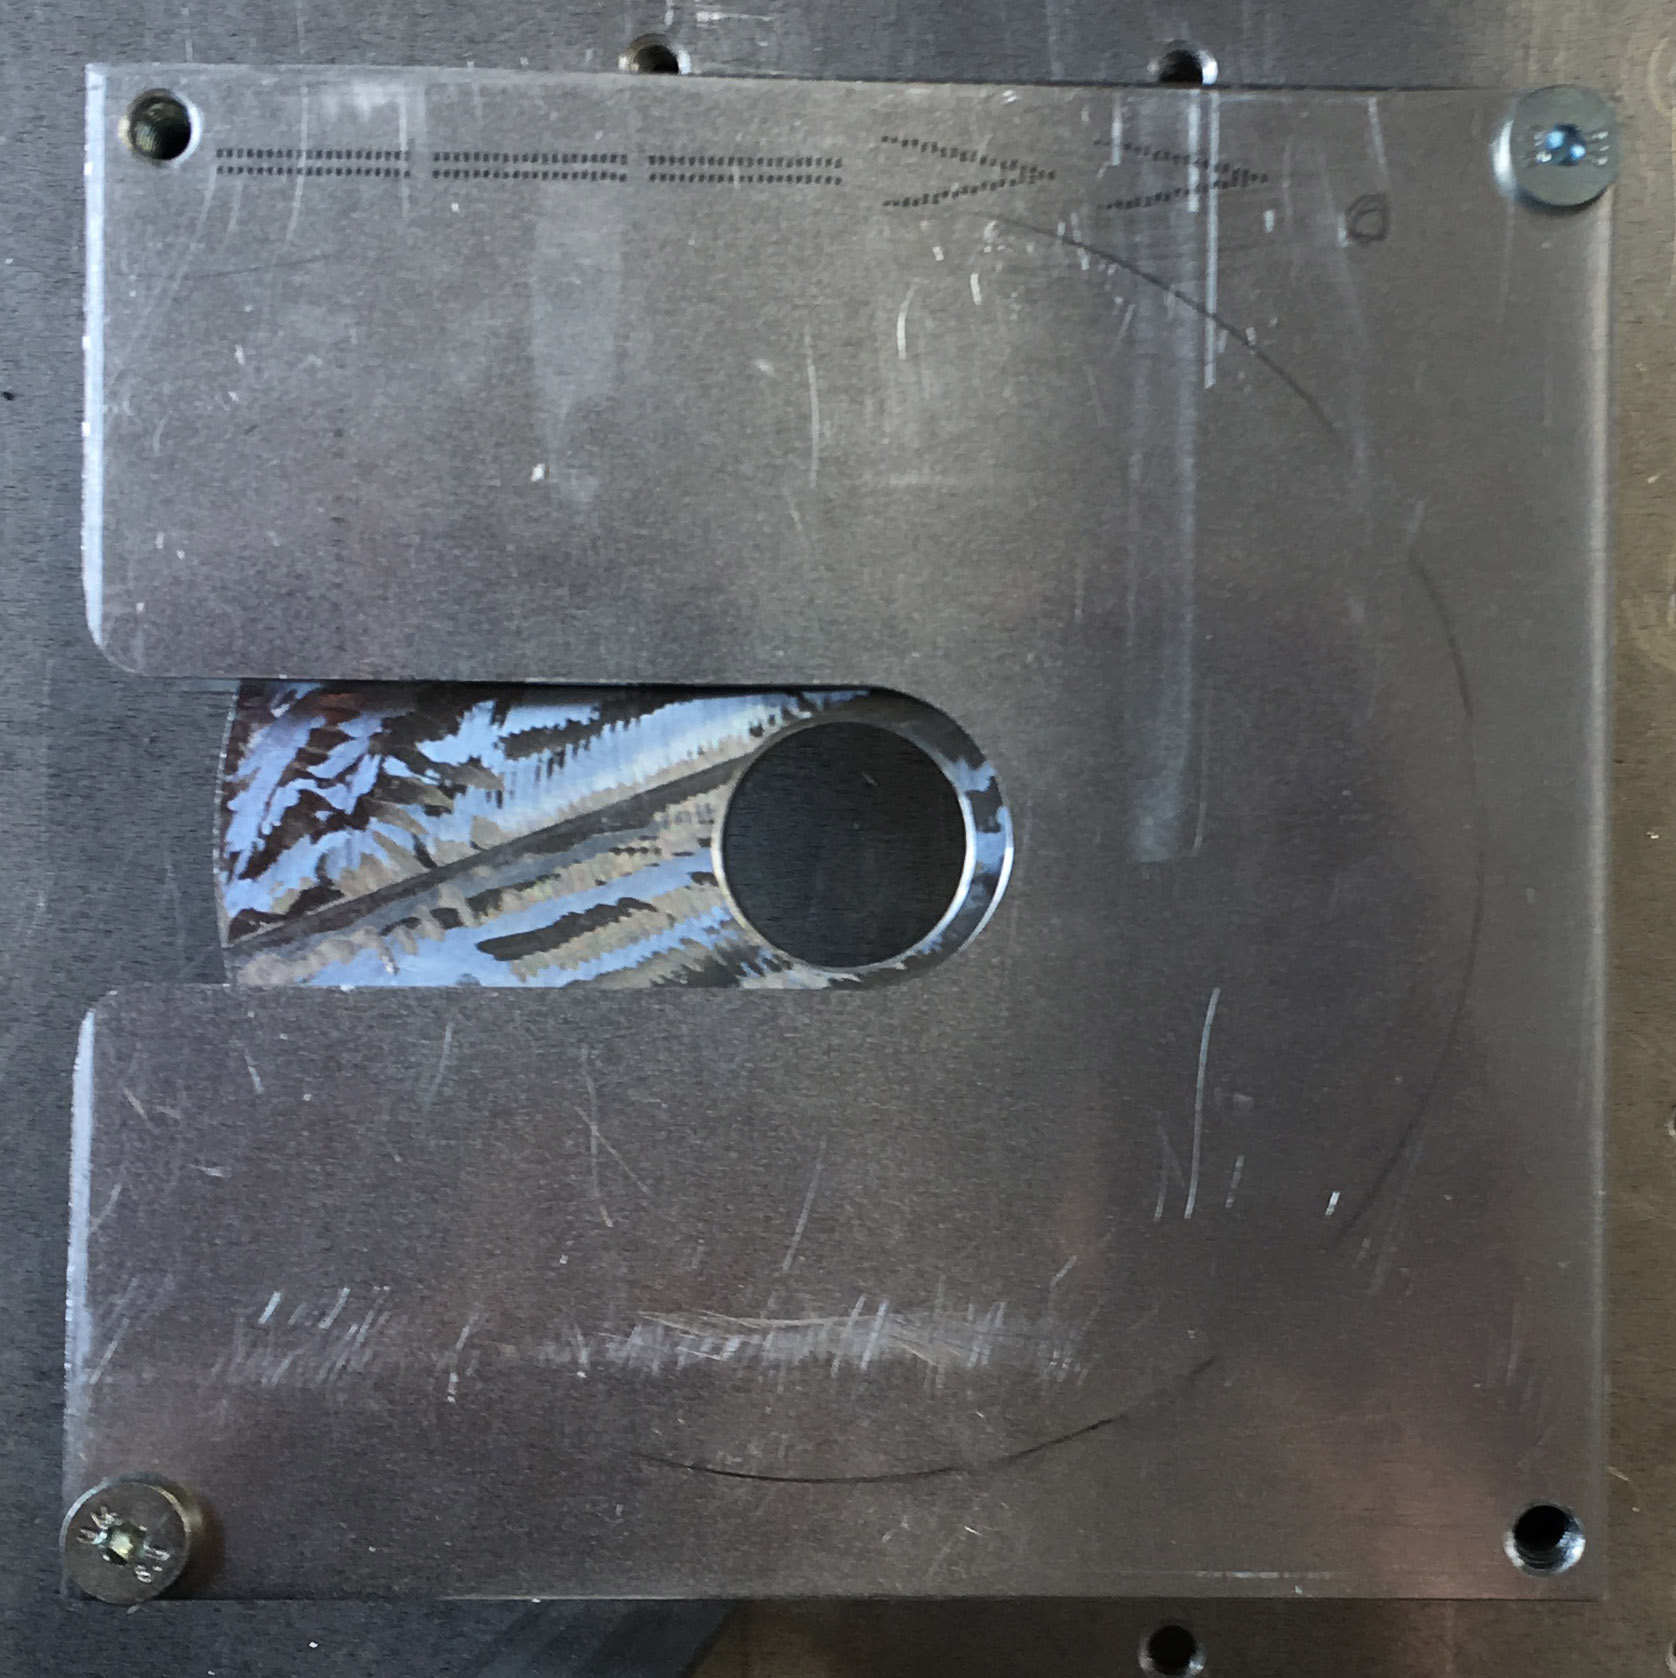
\includegraphics[width=1\textwidth]{pictures/rep_top_view}
   \caption[Finished \acs{Repository} top view]{Finished \acs{Repository} top view\\
	Source: Group 4  
   }
   \label{fig:rep_top_view}
\end{figure} 

  \begin{figure}[H]
  \centering
   \includegraphics[width=1\textwidth]{pictures/rep_side_view}
   \caption[Finished \acs{Repository} side view]{Finished \acs{Repository} side view\\
	Source: Group 4  
   }
   \label{fig:rep_side_view}
\end{figure} 

\newpage

\section{Electronic}
In \autoref{fig:electronic_1} the finished \acs{PCB} is shown with the connected \acs{uC} mounted on the Z-axis.
\begin{figure}[H]
  \centering
   \includegraphics[width=1\textwidth]{pictures/electronic_1}
   \caption[Finished electronic parts]{Finished electronic parts\\
	Source: Group 4  
   }
   \label{fig:electronic_1}
\end{figure} 


\section{Force Measurement}
In \autoref{fig:cycle_pick} and \autoref{fig:cylce_drop} are the force shown of each cycle.
\begin{figure}[H]
  \centering
   \includegraphics[width=1\textwidth]{pictures/cylce_drop}
   \caption[Force measurement drop cycle]{Force measurement drop cycle\\
	Source: Group 4  
   }
   \label{fig:cylce_drop}
\end{figure} 

\begin{figure}[H]
  \centering
   \includegraphics[width=1\textwidth]{pictures/cycle_pick}
   \caption[Force measurement pick cycle]{Force measurement pick cycle\\
	Source: Group 4  
   }
   \label{fig:cycle_pick}
\end{figure} 


\chapter{Discussion}

In this chapter there will be given some problems that were faced during this project and how they were approached and solved.\\
For the mechanical part of this projects two problems occurred that affected the progress of the project. The first problem that was faced was the purchase of the linear axis which had to be bought with a shipment time of two weeks. This halted the progress for about two weeks and gave some time to focus more on the different aspects of the project like the \acs{Repository} and the manufacturing of the parts. And next there was a problem with the snap connection which was designed for the correct forces that were applied on it. The arms of the snapper are bended a little bit to the middle. Therefore the outer diameter of the snapper was just a little bit bigger than the hole in the disc. So the snapper was not able to hold the disc. The solution for this problem was a little aluminium rod with a diameter of $12mm$ which we set into the snap connector. This small rod bends the arms of the snapper to his original position and so the snapper was able to hold the disc.\\
Despite the problems that were faced for the mechanical part, the electronical part also suffered from some problems. The Atmel board and a DRV8711 broke shortly after the \acs{PCB} was designed and a new board had to be used, this was caused by an overvoltage on the board. Also multiple parts were fried during the testing of the board, this was caused by a faulty connection or a short circuit. This never broke the board down completely and did not give major setbacks. The biggest problem was, that a view “vias” on the \acs{PCB} did not conduct correctly. Therefore the charge pump of the DRV8711 did not work at the beginning when the board was recently manufactured. Moreover the pick and place machine did not solder two capacitors and the \enquote{MAX232}, therefore the board did not work correctly. This was caused by the charge pump because that did not work properly at the time.\\
As for the programming of the \acs{uC} and the \acs{PLC}the biggest problem was that we did not know how to use the \acs{ASF} library. But this was solved by using and studying the example programs that were provided by the Atmel studio.
Finally, we had some problems with the requirement document. It was not completely clear to us what we had to put in the document. This followed in editing the document several times which took some time. In the end the document was finished and we were all pleased with the result. In the end we changed some aspect of this document mostly because some names were changed during the project or that an extra safety principle was added in the use cases. Also we added some requirements about tolerances, this was done so this is also clear to the customer.
\newpage

% \bibliographystyle{unsrt}
% \bibliographystyle{alpha}
% \bibliographystyle{plain}
% \bibliographystyle{unsrtnat}
%\bibliographystyle{authordate3}
%\clearpage
%\phantomsection
%\addcontentsline{toc}{chapter}{Literaturverzeichnis}
%\bibliography{references} % references.bib ist die verwendete bibtex-datei


%\chapter*{[Evtl. Anhang]}
%\addcontentsline{toc}{chapter}{[Evtl. Anhang]}
%Formatvorlage für den Fließtext.


%\chapter*{Eidesstattliche Erklärung}
%\addcontentsline{toc}{chapter}{Eidesstattliche Erklärung}
%Ich erkläre hiermit an Eides statt, dass ich die vorliegende Bachelorarbeit selbstständig und ohne Benutzung anderer als der angegebenen Hilfsmittel angefertigt habe. Die aus fremden Quellen direkt oder indirekt übernommenen Stellen sind als solche kenntlich gemacht. Die Arbeit wurde bisher weder in gleicher noch in ähnlicher Form einer anderen Prüfungsbehörde vorgelegt und auch noch nicht veröffentlicht.
%
%\vspace{30mm}
%\noindent
%Verfasser/in\hfill                                       Unterschrift Verfasser/in
%
%\vspace{3mm}
%\noindent
%Dornbirn, am [Tag. Monat Jahr anführen]\hfill            Vor- und Nachname Verfasser/in
\appendix
\addcontentsline{toc}{chapter}{Appendix}
\chapter{Mechanics}
\section{Drawings}
\begin{landscape}
\includepdf[pages={1-}]{datasheets/mechanical/psi5321_asseblyAxisGes.pdf}
\includepdf[pages={1-}]{datasheets/mechanical/psi5321_disk.pdf}
\includepdf[pages={1-}]{datasheets/mechanical/psi5321_frame1.pdf}
\includepdf[pages={1-}]{datasheets/mechanical/psi5321_frame2.pdf}
\includepdf[pages={1-}]{datasheets/mechanical/psi5321_microfix.pdf}
\includepdf[pages={1-}]{datasheets/mechanical/psi5321_part1.pdf}
\includepdf[pages={1-}]{datasheets/mechanical/psi5321_Rackbar.pdf}
\includepdf[pages={1-}]{datasheets/mechanical/psi5321_snapConnV5.pdf}
\includepdf[pages={1-}]{datasheets/mechanical/psi5321_upperplate.pdf}
\includepdf[pages={1-}]{datasheets/mechanical/psi5321_lowerplate_target.pdf}
\end{landscape}
\section{Linear Axis}
\includepdf[pages={1-}]{datasheets/mechanical/DE_GL8_drylinSLT_screen.pdf}

\chapter{Electronics}
\section{Power Resistor}
\includepdf[pages={1-}]{datasheets/electronics/3W_0R050.pdf}
\section{DRV8711}
\includepdf[pages={1-}]{datasheets/electronics/drv8711.pdf}
\section{\acs{MOSFET} IRF520}
\includepdf[pages={1-}]{datasheets/electronics/IRF520.pdf}
\section{Force Sensor}
\includepdf[pages={1-}]{datasheets/electronics/kd24s.pdf}
\section{LM1086 Linear Voltage Regulator}
\includepdf[pages={1-}]{datasheets/electronics/lm1086.pdf}
\section{MAX232 \acs{RS232} Level Changer}
\includepdf[pages={1-}]{datasheets/electronics/max232.pdf}
\section{Schrack Relay}
\includepdf[pages={1-}]{datasheets/electronics/schrack.pdf}

\chapter{\acs{uC}}
 \lstset{
   basicstyle=\scriptsize\ttfamily,
   keywordstyle=\bfseries\ttfamily\color{orange},
   stringstyle=\color{green}\ttfamily,
   commentstyle=\color{middlegray}\ttfamily,
   emph={square}, 
   emphstyle=\color{blue}\texttt,
   emph={[2]root,base},
   emphstyle={[2]\color{yac}\texttt},
   showstringspaces=false,
   flexiblecolumns=false,
   tabsize=2,
   numbers=left,
   numberstyle=\tiny,
   numberblanklines=false,
   stepnumber=1,
   numbersep=11pt,
   xleftmargin=15pt,
   breaklines=true
 }
\section{Main Loop}
  \lstinputlisting
    [captionpos=t,language=c, caption=Main]
{listings/mainGrabtastic.c}
 
 \section{Library}
  \lstinputlisting
    [captionpos=t,language=c, caption=Header]
 {listings/config_focus_fhv.h}

\section{\acs{ASF} Library}

\href{http://www.atmel.com/images/atmel-42139-asf-manual-sam-d20_application-note_at03665.pdf}{Atmel \acs{ASF}}

\section{Register Settings Atmel}

\href{http://www.atmel.com/images/atmel-42129-sam-d20_datasheet.pdf}{Atmel SAM D20 Register Settings}

\chapter{\acs{PLC}}





\section{Program}
 \lstset{
   basicstyle=\scriptsize\ttfamily,
   keywordstyle=\bfseries\ttfamily\color{orange},
   stringstyle=\color{green}\ttfamily,
   commentstyle=\color{middlegray}\ttfamily,
   emph={square}, 
   emphstyle=\color{blue}\texttt,
   emph={[2]root,base},
   emphstyle={[2]\color{yac}\texttt},
   showstringspaces=false,
   flexiblecolumns=false,
   tabsize=2,
   numbers=left,
   numberstyle=\tiny,
   numberblanklines=false,
   stepnumber=1,
   numbersep=11pt,
   xleftmargin=15pt,
   breaklines=true
	language=Pascal}
	
\subsection{Allgemein}
\begin{lstlisting}[language=pascal, captionpos=t, caption=Allgemein]

(*safe the min and max value of the force*)
IF maxForceValuePos < acutalForceValue THEN
	maxForceValuePos := acutalForceValue;
END_IF
IF maxForceValueNeg > acutalForceValue THEN
	maxForceValueNeg := acutalForceValue;
END_IF

\end{lstlisting}


\subsection{Main}
\begin{lstlisting}[language=pascal, captionpos=t, caption=Main]
VAR CONSTANT 
	BufStart:INT:=  1;      // Start-Index
 	BufEnd:INT:=  100;   // End-Index
END_VAR

VAR
	diX, diY AT %I* : BOOL;
	(*boole variables*)
	bStart :BOOL := FALSE;
	bMoveHome : BOOL := FALSE;
	bDauerlauf : BOOL := FALSE;
	i: INT;
	btest : BOOL;
	btestZwei : bool;
	btesDrei: BOOL;
END_VAR

posAxisX(Axis:= axisX, Enable:= TRUE , Valid=> , Busy=> , Error=> , ErrorID=> , Position=> );
posAxisY(Axis:= axisY, Enable:= TRUE, Valid=> , Busy=> , Error=> , ErrorID=> , Position=> );

powerX(Axis:= axisX, Enable:= bEnable, Enable_Positive:= bEnable, Enable_Negative:= bEnable, Override:= 100, BufferMode:= , Options:= , Status=> , Busy=> , Active=> , Error=> , ErrorID=> );
powerY(Axis:= axisY, Enable:= bEnable, Enable_Positive:= bEnable, Enable_Negative:= bEnable, Override:= 100, BufferMode:= , Options:= , Status=> , Busy=> , Active=> , Error=> , ErrorID=> );

resetX(Axis:= axisX, Execute:= , Done=> , Busy=> , Error=> , ErrorID=> );
resetY(Axis:= axisY, Execute:= , Done=> , Busy=> , Error=> , ErrorID=> );

homeX(Axis:= axisX, Execute:= , Position:= 0 , HomingMode:= , BufferMode:= , Options:= , bCalibrationCam:= NOT diX, Done=> , Busy=> , Active=> , CommandAborted=> , Error=> , ErrorID=> );
homeY(Axis:= axisY, Execute:= , Position:= 0 , HomingMode:= , BufferMode:= , Options:= , bCalibrationCam:= NOT diY, Done=> , Busy=> , Active=> , CommandAborted=> , Error=> , ErrorID=> );	

moveAbsX(Axis:= axisX, Execute:= , Position:= , Velocity:= , Acceleration:= , Deceleration:= , Jerk:= , BufferMode:= , Options:= , Done=> , Busy=> , Active=> , CommandAborted=> , Error=> , ErrorID=> );

moveAbsY(Axis:= axisY, Execute:= , Position:= , Velocity:= , Acceleration:= , Deceleration:= , Jerk:= , BufferMode:= buffermoveAbsY, Options:= , Done=> , Busy=> , Active=> , CommandAborted=> , Error=> , ErrorID=> );

moveAbsNewY(Axis:= axisY, Execute:= , Position:= , Velocity:= , Acceleration:= , Deceleration:= , Jerk:= , BufferMode:= buffermoveAbsY, Options:= , Done=> , Busy=> , Active=> , CommandAborted=> , Error=> , ErrorID=> );	

SCL(Crtl:= , bSend:= , ReceivedString=> , bNewString=> , bSendBusy=> , bStringReceived=> );
	
	rTrigStartCycle(CLK:= bStart , Q=> );
	CASE iState OF
		
	0:	IF (*rTrig.Q AND *)powerX.Status AND powerY.Status THEN
			iState := iState + 1;
		END_IF

	1:	SCL.Crtl := 'I';
		SCL.bSend := TRUE;
		respondOfORder := '';
		istate := 2;

	2:	IF NOT SCL.bSendBusy THEN
			SCL.bSend := FALSE;
			istate := 3;
		END_IF

	3:	IF waitToLongForRespond.Q THEN
			istate := 1;
		END_IF
		IF respondI.Q1 THEN
			respondI.RESET := TRUE;
			respondI.SET1 := FALSE;
			istate := 5;
		END_IF	
	
	5:		resetX.Execute :=TRUE;
			resetY.Execute :=TRUE;
			iState := 10;
		
	10:	IF resetX.Done AND resetY.Done THEN
			resetX.Execute := FALSE;
			resetY.Execute := FALSE;
			iState :=  iState + 5;
		END_IF
		
	15: IF NOT readInfoAxisX.Status.Homed or NOT readInfoAxisY.Status.Homed THEN
		homeX.Execute := TRUE;
		homeY.Execute := TRUE;
		iState := 20;
		ELSE
			iState := 21; //--> if already referenced, go home position
		END_IF
	20:	IF homeX.Done AND homeY.Done THEN
			homeX.Execute := FALSE;
			homeY.Execute := FALSE;
			NotHomed.RESET := FALSE;
			iState := 21;		
		END_IF
	21:			moveAbsY.Velocity := posHomeVelocityY;
				moveAbsY.Position := posHomeY;
				moveAbsY.Execute := TRUE;

			IF posAxisY.Position > posPrepositioningY THEN
				moveAbsX.Velocity := posHomeVelocityX;
				moveAbsX.Position := posHomeX;
				moveAbsX.Execute := TRUE;
				iState :=  25;
			END_IF

	25:	IF 	moveAbsX.Done AND moveAbsY.Done THEN
			moveAbsX.Execute:= FALSE;
			moveAbsY.Execute:= FALSE;
			respondH.RESET := TRUE;
			respondH.SET1 := FALSE;
			iState :=  26;
		END_IF
		
	(*this starts a new cycle, depending on the load*)
	26:	IF rTrigStartCycle.Q OR bDauerlauf THEN
			IF bLoaded THEN
				iState :=  125;
			ELSE
				iState :=  27;
			END_IF
			respondD.RESET := TRUE;
			respondD.SET1 := FALSE;
			respondH.RESET := TRUE;
			respondH.SET1 := FALSE;
			respondP.RESET := TRUE;
			respondP.SET1 := FALSE;
			cycleFinished := FALSE;
		END_IF				
		
	27:		moveAbsX.Velocity := posRepositoryVelocityX;
			moveAbsX.Position := posRepositoryX;
			moveAbsX.Execute := TRUE;
			moveAbsY.Velocity := posRepositoryVelocityY;
			moveAbsY.Position :=posRepositoryY;
			moveAbsY.Execute := TRUE;
			iState :=  28;
			maxForceValuePos := 0;
			maxForceValueNeg := 0;

	28: 	SCL.Crtl := 'P'; // vorpositionieren
			SCL.bSend := TRUE;
			iState :=  29;
		
	29:	IF NOT SCL.bSendBusy THEN
			SCL.bSend := FALSE;
			SCL.Crtl := '';
			istate := 30;
		END_IF
		
	30:	IF waitToLongForRespond.Q THEN
			istate := 28;
			END_IF
		IF 	moveAbsX.Done AND moveAbsY.Done AND respondP.Q1 THEN
			moveAbsX.Execute:= FALSE;
			moveAbsY.Execute:= FALSE;
			respondP.RESET := TRUE;
			respondP.SET1 := FALSE;
			iState := 31;
		END_IF
		
	31:	SCL.Crtl := 'D';
		SCL.bSend := TRUE;
		istate := 32;
		
	32:	IF NOT SCL.bSendBusy THEN
			SCL.bSend := FALSE;
			SCL.Crtl := '';
			istate := 33;
		END_IF

	33:	IF waitToLongForRespond.Q THEN
			istate := 31;
			END_IF
		IF respondD.Q1 THEN //Move Down
			respondD.RESET := TRUE;
			respondD.SET1 := FALSE;
			bLoaded := TRUE;
			cycleFinished :=TRUE;
			istate := 35;
		END_IF	
		
	35:		IF NOT respondD.Q1 THEN
				moveAbsY.Velocity := posHomeVelocityY;
				moveAbsY.Position :=posHomeY;
				moveAbsY.Execute := TRUE;
			IF posAxisY.Position > posPrepositioningY THEN //über dem weg drausen, dan darf er fahren
				moveAbsX.Velocity := posHomeVelocityX;
				moveAbsX.Position := posHomeX;
				moveAbsX.Execute := TRUE;
				iState :=  40;
			END_IF
		
		END_IF
	40:	IF 	moveAbsX.Done AND moveAbsY.Done THEN
			moveAbsX.Execute:= FALSE;
			moveAbsY.Execute:= FALSE;
			iState := 26;
		END_IF
		
	125:	moveAbsX.Velocity := 5;
			moveAbsX.Position := posPrepositioningX;
			moveAbsX.Execute := TRUE;
			moveAbsY.Velocity := posPrepositioningVelocityY;
			moveAbsY.Position :=posPrepositioningY;
			moveAbsY.Execute := TRUE;
			iState :=  130;
			maxForceValuePos := 0;
			maxForceValueNeg := 0;
			
	130:	IF moveAbsX.Done THEN
				moveAbsNewY.Execute:= TRUE;
				moveAbsNewY.Velocity := posRepositoryVelocityY;
				moveAbsNewY.Position := posRepositoryY;
				moveAbsY.Execute:= FALSE;
				moveAbsX.Execute:= FALSE;
			END_IF
			IF moveAbsNewY.Done THEN
				iState := 140;
		END_IF
		
	(*135:	moveAbsX.Velocity := 	posRepositoryVelocityX;
			moveAbsX.Position := 	posRepositoryX;
			moveAbsX.Execute := 	TRUE;
			moveAbsY.Velocity :=	posRepositoryVelocityY;
			moveAbsY.Position :=	posRepositoryY;
			moveAbsY.Execute := TRUE;
			iState :=  140;*)
			
	140:	IF 	(*moveAbsX.Done AND*) moveAbsNewY.Done THEN
			moveAbsNewY.Execute:= FALSE;
			iState :=  141;
			END_IF
			
	141:	SCL.Crtl := 'P'; //Move Up
			SCL.bSend := TRUE;
			istate := 142;
			
	142:	IF NOT SCL.bSendBusy THEN
			SCL.bSend := FALSE;
			SCL.Crtl := '';
			istate := 143;
		END_IF

	143:	IF waitToLongForRespond.Q THEN
				istate := 141;
			END_IF
			IF respondP.Q1 THEN
				respondP.RESET := TRUE;
				respondP.SET1 := FALSE;
				bLoaded := FALSE;
				cycleFinished :=TRUE;
				iState := 145;
			END_IF	
			
	145:	SCL.Crtl := 'H'; // Home pos anfahren
			SCL.bSend := TRUE;
			iState :=  150;
		
	150:	IF NOT SCL.bSendBusy THEN
				SCL.bSend := FALSE;
				SCL.Crtl := '';
				istate := 155;
			END_IF

 	155:	moveAbsY.Velocity := posHomeVelocityY;
				moveAbsY.Position := posHomeY;
				moveAbsY.Execute := TRUE;

			IF posAxisY.Position > posPrepositioningY THEN
				moveAbsX.Velocity := posHomeVelocityX;
				moveAbsX.Position := posHomeX;
				moveAbsX.Execute := TRUE;
				iState :=  160;
			END_IF
		
	160:	IF waitToLongForRespond.Q THEN
				istate := 145;
			END_IF
			IF 	moveAbsX.Done AND moveAbsY.Done AND respondH.Q1 THEN
			moveAbsX.Execute:= FALSE;
			moveAbsY.Execute:= FALSE;
			respondH.RESET := TRUE;
			respondH.SET1 := FALSE;
			iState :=  26;
		END_IF
		
	END_CASE
	
	resetErrorHandling();
	visu();
\end{lstlisting}
\subsection{Error and Reset}

\begin{lstlisting}[language=pascal, captionpos=t, caption=Error and Reset]
VAR
	reset: INT := 0; //reset state machine
END_VAR

VAR CONSTANT 
	toMuchForcePositive : INT := 15000;
	toMuchForceNegative : INT := -15000;
END_VAR

respondD(SET1:= , RESET:= , Q1=> );
respondH(SET1:= , RESET:= , Q1=> );
respondI(SET1:= , RESET:= , Q1=> );
respondP(SET1:= , RESET:= , Q1=> );
respondOk(SET1:= , RESET:= , Q1=> );
respondStartetUp(SET1:= , RESET:= , Q1=> );
emergencyStopToMuchForce(SET1:= , RESET:= , Q1=> );
motorXYNoPower(SET1:= , RESET:= , Q1=> );
errorNoSignalFromUc(SET1:= , RESET:= , Q1=> );
unequalLoadThanExpected(SET1:= , RESET:= , Q1=> );
zAxisNotMoving(SET1:= , RESET:= , Q1=> );

rTrigStartViewPressed(CLK:= bStartViewPressed , Q=> );

IF respondI.Q1 THEN
		respondI.SET1 := FALSE;
END_IF

respondD.RESET := FALSE;
respondH.RESET := FALSE;
respondI.RESET := FALSE;
respondP.RESET := FALSE;
respondOK.RESET := FALSE;
respondStartetUp.RESET := FALSE;
emergencyStopToMuchForce.RESET := FALSE;
motorXYNoPower.RESET := FALSE;
errorNoSignalFromUc.RESET := FALSE;
unequalLoadThanExpected.RESET := FALSE;
zAxisNotMoving.RESET:=FALSE;

(*read status from x and y*)
readInfoAxisX(Axis:= axisX, Enable:= TRUE, Valid=> , Busy=> , Error=> , ErrorID=> , ErrorStop=> , Disabled=> , Stopping=> , StandStill=> , DiscreteMotion=> , ContinuousMotion=> , SynchronizedMotion=> , Homing=> , ConstantVelocity=> , Accelerating=> , Decelerating=> , Status=> );
readInfoAxisY(Axis:= axisY, Enable:= TRUE, Valid=> , Busy=> , Error=> , ErrorID=> , ErrorStop=> , Disabled=> , Stopping=> , StandStill=> , DiscreteMotion=> , ContinuousMotion=> , SynchronizedMotion=> , Homing=> , ConstantVelocity=> , Accelerating=> , Decelerating=> , Status=> );

(* wait to seconds to give the stepper motor drivers a little time to built DC link*)
waitWithEnable(IN:= bEmergencyPressed, PT:= T#2S, Q=> , ET=> );

(* if no respond from the uC in a little time, the nsend command again*)
waitToLongForRespond(IN:= 	iState = 33  OR iState = 143 OR iState =3 OR iState = 30, PT:= T#10S, Q=> , ET=> );

zAxisNotMoving.SET1:= (globalErrorFromUC = '2E');

(* Ungleich soll beladung *)
IF (iState = 23 OR iState = 0) AND ((acutalForceValue > -200 AND bLoaded) OR (acutalForceValue < -700 AND NOT bLoaded))THEN
	unequalLoadThanExpected.SET1:=TRUE;
END_IF

(* error if no respond from uC*)
errorNoSignalFromUc.SET1 := NOT noSiganlFromU.Q;

(* trigger after restart from emergency *)
fTrigReset(CLK:= waitWithEnable.Q, Q=> );

(* set if we ar not homed*)
NotHomed(SET1:= NOT readInfoAxisX.Status.Homed OR NOT readInfoAxisY.Status.Homed, RESET:= , Q1=> );
motorXYNoPower.SET1 :=  readInfoAxisY.ErrorStop OR readInfoAxisX.ErrorStop;
(* Status not ok but Emergency is ok*)
globalErrorDetect := motorXYNoPower.Q1 OR respondStartetUp.Q1 OR emergencyStopToMuchForce.Q1 OR bEmergencyPressed OR errorNoSignalFromUc.Q1 OR unequalLoadThanExpected.Q1 OR zAxisNotMoving.Q1;
(* set error *)
setError(SET1:=globalErrorDetect, RESET:= , Q1=> );

CASE reset OF
0:	IF fTrigReset.Q OR ((setError.Q1 OR NotHomed.SET1) AND (bReset OR rTrigStartViewPressed.Q)) THEN
		reset := 5;
		iState := 0;
		bEnable := FALSE;
		globalErrorDetect := FALSE;
		setError.RESET :=TRUE;
		respondStartetUp.RESET := TRUE;
		bLoaded := FALSE;
		respondStartetUp.SET1 := FALSE;
		emergencyStopToMuchForce.RESET := TRUE;
		emergencyStopToMuchForce.SET1 := FALSE;
		motorXYNoPower.SET1 := FALSE;
		motorXYNoPower.RESET := TRUE;
		errorNoSignalFromUc.SET1 := FALSE;
		errorNoSignalFromUc.RESET := TRUE;
		unequalLoadThanExpected.SET1:= FALSE;
		unequalLoadThanExpected.RESET := TRUE;
		zAxisNotMoving.SET1 := FALSE;
		zAxisNotMoving.RESET := TRUE;
		respondI.RESET := TRUE;
		respondI.SET1 := FALSE;
		respondD.RESET := TRUE;
		respondD.SET1 := FALSE;
		respondH.RESET := TRUE;
		respondH.SET1 := FALSE;
		maxForceValuePos := 0;
		maxForceValueNeg := 0;
	END_IF
5:	resetX.Execute :=TRUE;
	resetY.Execute :=TRUE;
	setError.RESET :=FALSE;
	reset := 10;
	
10:	IF resetX.Done AND resetY.Done THEN
		resetX.Execute := FALSE;
		resetY.Execute := FALSE;
		reset :=  15;
	END_IF
15: bEnable := TRUE;
	reset  := 0;
END_CASE

(* if to much force --> emergency stop!*)
IF (acutalForceValue > toMuchForcePositive) OR (acutalForceValue < toMuchForceNegative) THEN
	emergencyStopToMuchForce.SET1 := TRUE;
END_IF



(*reset all movements and sending*)
IF setError.Q1 THEN
	iState := 0;
	homeX.Execute := FALSE;
	homeY.Execute := FALSE;
	moveAbsX.Execute:= FALSE;
	moveAbsY.Execute:= FALSE;
	moveAbsNewY.Execute:= FALSE;
	bEnable := FALSE;
	SCL.bSend := FALSE;
	SCL.Crtl := '';
END_IF

\begin{lstlisting}[language=pascal]
\end{lstlisting}



\subsection{Serial Com}
\begin{lstlisting}[language=pascal, captionpos=t, caption=Serial Communication]
VAR_INPUT
	Crtl: STRING;
	bSend: BOOL;
END_VAR
VAR_OUTPUT
	ReceivedString: STRING;
	bNewString: BOOL;
	bSendBusy: BOOL;
	bStringReceived: BOOL;
END_VAR
(*VAR_IN_OUT
	IOrespondOfORder: STRING;
END_VAR*)
VAR
	//DataIn AT %I*: EL6inData22B;
	//DataOut AT %Q*: EL6outData22B;
	SerialLineCtrl: SerialLineControl;
	//BuffTX: ComBuffer;
	//BuffRX: ComBuffer;
	clearbuff: ClearComBuffer;
	SendString: SendString;
	RecString: ReceiveString;
	istate: INT;
	rtrig: r_trig;
	test: ReceiveByte;
	bTest: BYTE;
	bByteReceived : BOOL := FALSE;
	bBuffer: BYTE;
	arrForceValues : ARRAY [1..1000] OF INT;

	lengtOfReceivedString: INT;
	strTemp : STRING(255);
	posSuffix: INT;
	stest :STRING;
	
	posFirstSlash: INT;
	posSecondSlash: INT;
	posThirdSlash: INT;
	posHash: INT;
END_VAR


SendString(SendString:= , Busy=> , Error=> , TXbuffer:= BuffTX);
RecString(Prefix:= , Suffix:= '$N', Timeout:= T#2S, Reset:= , StringReceived=> , 	Busy=> , 	Error=> , 	RxTimeout=> , 	ReceivedString:= ReceivedString, 	RXbuffer:= BuffRX);
posHash := FIND (ReceivedString,'#');
posSuffix := FIND (ReceivedString,'$R');
posFirstSlash := FIND (ReceivedString,'/');
strTemp := MID (ReceivedString,posSuffix - posFirstSlash-1,posFirstSlash+1);
posSecondSlash := FIND (strTemp,'/') + posFirstSlash;
strTemp := MID (ReceivedString,posSuffix - posSecondSlash-1,posSecondSlash+1);
posThirdSlash := FIND (strTemp,'/') + posSecondSlash;

lengtOfReceivedString:=LEN(STR:= ReceivedString);

IF RecString.StringReceived THEN
	strTemp := MID (ReceivedString,posSecondSlash - posHash-1,posHash+1);
	acutalForceValue := STRING_TO_INT (strTemp);
	
	strTemp := MID (ReceivedString,posThirdSlash - posSecondSlash-1,posSecondSlash+1);
	posAxisZ := STRING_TO_INT (strTemp);

	globalErrorFromUC := MID (ReceivedString,posSuffix - posThirdSlash-1,posThirdSlash+1);
	
	globalForceValueArrived := TRUE;
	RecString.Reset := TRUE;

	respondOfORder := MID (ReceivedString,posFirstSlash-1,1); (* else its a respond of the Order*)
	RecString.Reset := TRUE;
	respondI.SET1 := respondOfORder = 'i';
	respondH.SET1 := respondOfORder = 'h';
	respondD.SET1 := respondOfORder = 'd';
	respondP.SET1 := respondOfORder = 'p';
	respondOK.SET1 := respondOfORder = 'ok';
	respondStartetUp.SET1 :=  respondOfORder  = 'Started up';
	respondOfORder := '';
	counterSerialCom := counterSerialCom+1;
END_IF


(* no isgnal from uC *)
noSiganlFromU(IN:= RecString.StringReceived, PT:= T#2S, Q=> , ET=> );


rtrig(CLK:= bSend, Q=> );
CASE istate OF

0:	RecString.Reset := FALSE;
	bStringReceived := FALSE;
	IF rtrig.Q THEN
		SendString.SendString := Crtl;
		bSendBusy := TRUE;
		istate := istate  + 1;
	END_IF	

1:	IF NOT SendString.Busy THEN
			SendString.SendString := '';
			(*clearbuff(Buffer:= BuffTX );*)
			istate := istate + 1;
			ReceivedString := '';
			bSendBusy := FALSE;
	END_IF

2:	IF RecString.StringReceived THEN
		bStringReceived := TRUE;
		RecString.Reset := TRUE;
		istate := 0;
	END_IF
		
END_CASE


\end{lstlisting}

\subsection{Visualization}
\begin{lstlisting}[language=pascal, captionpos=t, caption=Visualization]
VAR
	//stringErrorText : WSTRING; //error texts for visu
	//stringMessageText : WSTRING;
	//stringDebugText : WSTRING;
	stringErrorText: ARRAY [1..20] OF STRING;
	stringMessageText: ARRAY [1..20] OF STRING;
	stringDebugText: ARRAY [1..20] OF STRING;
	forceMemoryDrop: writeInArray;
	forceMemoryPick: writeInArray;
	zaehl: INT := 1;
END_VAR

forceMemoryDrop(i_iState:= iState, i_actualForceValue:= acutalForceValue, i_bLoaded:= TRUE, io_ValueArrived:= globalForceValueArrived);
forceMemoryPick(i_iState:= iState, i_actualForceValue:= acutalForceValue, i_bLoaded:= FALSE, io_ValueArrived:= globalForceValueArrived);
//cycleFinished(SET1:= , RESET:= , Q1=> );

(* pos of x and y for the visu*)
IF readInfoAxisX.Status.Homed AND readInfoAxisY.Status.Homed	THEN
realVisuPosX := posAxisX.Position * 1.5;
realVisuPosY := (posAxisY.Position * (-1.0) + 10) *1.7;
//realVisuPosX := ABS (realVisuPosX);
ELSE
realVisuPosX := 0.0;
realVisuPosY := 0.0;	
END_IF

IF bLoaded THEN
	realVisuDiskX := realVisuPosX; (* - posRepositoryX * 1.5;*)
	realVisuDiskY := realVisuPosY; (*- (posRepositoryY * (-1.0) + 10) *2.0;	*)
ELSE
	realVisuDiskX := posRepositoryX * 1.5;
	realVisuDiskY := (posRepositoryY * (-1.0) + 10) *2.0;
END_IF

IF iState > 3 THEN
intVisuPosZ := (posAxisZ) *2;
ELSE
intVisuPosZ := 0;	
END_IF

(*prepare cycle finished*)

(* visu texts *)

MEMSET(ADR(stringErrorText), 0, SIZEOF(stringErrorText));
MEMSET(ADR(stringMessageText), 0, SIZEOF(stringMessageText));
MEMSET(ADR(stringDebugText), 0, SIZEOF(stringDebugText));

zaehl := 1;
(* error messages *)
IF NOT readInfoAxisX.Status.Homed OR NOT readInfoAxisY.Status.Homed THEN
	stringErrorText[zaehl]:= CONCAT(STR1:= stringErrorText[zaehl], STR2:= 'Not referenced in X/Y');
	zaehl := zaehl + 1;
END_IF

IF  globalErrorDetect THEN
	stringErrorText[zaehl]:= CONCAT(STR1:= stringErrorText[zaehl], STR2:= 'Failure');
	zaehl := zaehl + 1;
END_IF

IF  bEmergencyPressed THEN
	stringErrorText[zaehl]:= CONCAT(STR1:= stringErrorText[zaehl], STR2:= 'Emergency Stop');
	zaehl := zaehl + 1;
END_IF

IF  emergencyStopToMuchForce.Q1 THEN
	stringErrorText[zaehl]:= CONCAT(STR1:= stringErrorText[zaehl], STR2:= 'too much Force');
	zaehl := zaehl + 1;
END_IF

IF motorXYNoPower.Q1 THEN
	stringErrorText[zaehl]:= CONCAT(STR1:= stringErrorText[zaehl], STR2:= 'Not referenced in X/Y');	
	zaehl := zaehl + 1;
END_IF

IF errorNoSignalFromUc.Q1 THEN
	stringErrorText[zaehl]:= CONCAT(STR1:= stringErrorText[zaehl], STR2:= 'error connection lost to uC');
	zaehl := zaehl + 1;
END_IF

IF unequalLoadThanExpected.Q1 THEN
	stringErrorText[zaehl]:= CONCAT(STR1:= stringErrorText[zaehl], STR2:= 'load unequal than expected');	
	zaehl := zaehl + 1;
END_IF

IF zAxisNotMoving.Q1 THEN
	stringErrorText[zaehl]:= CONCAT(STR1:= stringErrorText[zaehl], STR2:= 'z-axis Error');	
	zaehl := zaehl + 1;
END_IF

(* massage textes *)
	zaehl := 1;
IF acutalForceValue > -200  THEN
	stringMessageText[zaehl]:= CONCAT(STR1:= stringMessageText[zaehl], STR2:= 'The object is successfully dropped');
	zaehl := zaehl + 1;
END_IF

IF acutalForceValue < -700 THEN
	stringMessageText[zaehl]:= CONCAT(STR1:= stringMessageText[zaehl], STR2:= 'The object is successfully grabbed');
	zaehl := zaehl + 1;
END_IF


IF iState = 26 AND cycleFinished THEN
	stringMessageText[zaehl]:= CONCAT(STR1:= stringMessageText[zaehl], STR2:= 'Cycle successfully finished');
	zaehl := zaehl + 1;
END_IF

(* debug messages *)
	zaehl := 1;
IF bLoaded THEN	
	stringDebugText[zaehl]:= CONCAT(STR1:= stringDebugText[zaehl], STR2:= 'Load');
	zaehl := zaehl + 1;
ELSE
	stringDebugText[zaehl]:= CONCAT(STR1:= stringDebugText[zaehl], STR2:= 'No Load');
	zaehl := zaehl + 1;
END_IF

stringDebugText[zaehl]:= CONCAT(STR1:= stringDebugText[zaehl], STR2:= 'State PLC: ');
stringDebugText[zaehl]:= CONCAT(STR1:= stringDebugText[zaehl], STR2:= INT_TO_STRING (iState));
zaehl := zaehl + 1;
stringDebugText[zaehl]:= CONCAT(STR1:= stringDebugText[zaehl], STR2:= 'Error from uC:');
stringDebugText[zaehl]:= CONCAT(STR1:= stringDebugText[zaehl], STR2:= globalErrorFromUC);
zaehl := zaehl + 1;

\end{lstlisting}

\subsection{Write in Array}
\begin{lstlisting}[language=pascal, captionpos=t, caption=Write in Array]
VAR CONSTANT 
	BufStart:INT:=  1;      // Start-Index
 	BufEnd:INT:=  100;   // End-Index
END_VAR

VAR_INPUT
	i_iState : INT;
	i_actualForceValue : INT;
	i_bLoaded : BOOL;
END_VAR
VAR_OUTPUT
	
END_VAR
VAR
	sTemp : INT;
	sArrForceValue: ARRAY [BufStart..BufEnd] OF INT;
END_VAR

VAR_IN_OUT
	io_ValueArrived : BOOL;
END_VAR


IF io_ValueArrived AND ((NOT i_bLoaded AND (iState = 33) AND (posAxisZ > 60 )) OR (i_bLoaded AND (iState = 143) AND (posAxisZ > 57 ))) THEN
		sTemp := sTemp + 1;
		IF sTemp > BufEnd THEN
			sTemp:=1;
		END_IF
		sArrForceValue[sTemp] := i_actualForceValue;
		io_ValueArrived := FALSE;		
	END_IF
	
	IF	(((i_iState = 27 AND NOT i_bLoaded) OR (i_iState = 125 AND i_bLoaded)) ) THEN //delet Buffer Begin from new
		MEMSET(ADR(sArrForceValue), 0, SIZEOF(sArrForceValue));
		sTemp:=1;
	END_IF

\end{lstlisting}

\section{Datasheets}

\includepdf[pages={1-}]{datasheets/PLC/Product_Overview_NOE2-2.pdf}
\includepdf[pages={1-}]{datasheets/PLC/ST5918M3008-A.pdf}

\end{document}
